\documentclass{article}
\usepackage[utf8]{inputenc}
\usepackage[T5]{fontenc} % Font tiếng Việt
\usepackage[fontsize=13pt]{scrextend} % Set fontsize=13pt
% --- Gói tạo bảng co giãn ---
\usepackage{tabularx} 

% --- Gói màu sắc cho bảng (QUAN TRỌNG: phải có tùy chọn [table]) ---
\usepackage[table]{xcolor}
% --- Hiển thị code đẹp ---
\usepackage{listings}

\definecolor{codebg}{RGB}{248,248,248}
\definecolor{codegray}{RGB}{90,90,90}
\definecolor{codeblue}{RGB}{0,80,160}
\definecolor{codegreen}{RGB}{0,130,70}
\definecolor{codered}{RGB}{170,60,60}

\lstdefinestyle{matlabstyle}{
    language=Matlab,
    backgroundcolor=\color{codebg},
    basicstyle=\ttfamily\small,
    keywordstyle=\color{codeblue}\bfseries,
    commentstyle=\color{codegreen}\itshape,
    stringstyle=\color{codered},
    numberstyle=\tiny\color{codegray},
    numbers=left,
    stepnumber=1,
    numbersep=8pt,
    frame=single,
    rulecolor=\color{black!25},
    breaklines=true,
    breakatwhitespace=true,
    tabsize=4,
    showstringspaces=false,
    captionpos=b,
    xleftmargin=1.5em,
    framexleftmargin=1.2em
}
% --- Cấu hình trang in ---
\usepackage[paperheight=29.7cm,paperwidth=21cm,right=2cm,left=3cm,top=2cm,bottom=2.5cm,twoside]{geometry}

% --- Font và Toán học ---
\usepackage{mathptmx} % Times New Roman
\usepackage{amsmath}
\usepackage{amssymb}
\usepackage{bm}
\usepackage{microtype}

% --- Đồ họa và bảng biểu ---
\usepackage{graphicx}
\usepackage{float}
\usepackage{tikz}
\usetikzlibrary{calc}
\usepackage{multicol,multirow,tabularx}
\usepackage{rotating}
\usepackage[font=bf]{caption}
\usepackage{xcolor} % <--- QUAN TRỌNG: Để dùng màu đỏ ở bìa
\usepackage{longtable}
\usepackage{enumitem}
% --- Định dạng tiêu đề ---
\usepackage{titlesec}
\setcounter{secnumdepth}{4} 

% Heading 1
\titleformat{\section}[hang]{\normalfont\fontsize{16pt}{19.2pt}\selectfont \bfseries \centering}{\thesection.}{1em}{}
\titlespacing*{\section}{0pt}{3.5ex plus 1ex minus .2ex}{2.3ex plus .2ex}

% Heading 2
\titleformat*{\subsection}{\fontsize{14pt}{16.8pt}\selectfont \bfseries}
\titlespacing*{\subsection}{0pt}{10pt}{0pt}

% Heading 3
\titleformat*{\subsubsection}{\fontsize{13pt}{15.6pt}\selectfont \bfseries \itshape}
\titlespacing*{\subsubsection}{0pt}{10pt}{0pt}

% Heading 4
\titleformat*{\paragraph}{\fontsize{13pt}{15.6pt}\selectfont \itshape}
\titlespacing*{\paragraph}{0pt}{10pt}{0pt}

% --- Cấu hình đoạn văn ---
\usepackage{indentfirst}
\renewcommand{\baselinestretch}{1.2} 
\setlength{\parskip}{6pt}
\setlength{\parindent}{1cm}

% --- Định nghĩa cột bảng ---
\newcolumntype{s}{>{\hsize=.3\hsize}X}
\newcolumntype{y}{>{\hsize=.4\hsize}X}
\newcolumntype{d}{>{\hsize=.1\hsize}X}
\newcolumntype{a}{>{\hsize=1.1\hsize}X}
\newcolumntype{g}{>{\hsize=5\hsize}X}
\newcolumntype{C}[1]{>{\hsize=#1\hsize\centering\arraybackslash}X}
\renewcommand{\tabularxcolumn}[1]{>{\small}m{#1}}

% --- Đánh số và Caption (Việt hóa) ---
\renewcommand{\figurename}{\fontsize{12pt}{0pt}\selectfont \bfseries Hình}
\renewcommand{\thefigure}{\thesection.\arabic{figure}}
\captionsetup[figure]{labelsep=space}

\renewcommand{\tablename}{\fontsize{12pt}{0pt}\selectfont \bfseries Bảng}
\renewcommand{\thetable}{\thesection.\arabic{table}}
\captionsetup[table]{labelsep=space}

\renewcommand{\theequation}{\thesection.\arabic{equation}}
\numberwithin{equation}{section}
\numberwithin{figure}{section}
\numberwithin{table}{section}

% --- Tiện ích ---
\usepackage{lipsum}
\renewcommand{\contentsname}{MỤC LỤC}
\usepackage[ddmmyyyy]{datetime}
\usepackage{nameref}
\usepackage[unicode]{hyperref}
\Urlmuskip=0mu plus 2mu\relax
\newcommand{\codepath}[1]{\begingroup\Urlmuskip=0mu plus 1mu\footnotesize\path{#1}\endgroup}

% ================= DOCUMENT =================
\begin{document}
\renewcommand{\labelitemi}{--} 
\renewcommand{\labelitemii}{-}
% 1. Gọi file Bìa
\thispagestyle{empty}
\begin{tikzpicture}[overlay,remember picture]
\draw [line width=3pt]
    ($ (current page.north west) + (3.0cm,-2.0cm) $)
    rectangle
    ($ (current page.south east) + (-2.0cm,2.5cm) $);
\draw [line width=0.5pt]
    ($ (current page.north west) + (3.1cm,-2.1cm) $)
    rectangle
    ($ (current page.south east) + (-2.1cm,2.6cm) $); 
\end{tikzpicture}

\begin{center}
\vspace{-12pt} 
\textbf{\fontsize{16pt}{19pt}\selectfont \textcolor{red}{HỌC VIỆN CÔNG NGHỆ BƯU CHÍNH VIỄN THÔNG}}\\
\textbf{\fontsize{15pt}{18pt}\selectfont KHOA KỸ THUẬT ĐIỆN TỬ 1}

\vspace{1cm}

\begin{figure}[H]
     \centering
     % Đảm bảo bạn có file logoPTIT.png trong thư mục Figures
     
\includegraphics[width=0.30\textwidth]{logoPTIT.png}
\end{figure}

\vspace{1cm}
\textbf{\fontsize{26pt}{31pt}\selectfont BÁO CÁO CUỐI KÌ}
\vspace{1.5cm} % Đã sửa dấu phẩy thành dấu chấm
\end{center}

\begin{center}
    \textbf{\fontsize{23pt}{28pt}\selectfont HỌC SÂU }
\vspace{1.2cm} % Đã sửa dấu phẩy thành dấu chấm

\begin{table}[H]
    \centering
    % Đã sửa p{6,5cm} thành p{6.5cm}
    \begin{tabular}{l l} 
    \fontsize{12pt}{14pt}\selectfont \textbf{Giảng viên:} & \fontsize{14pt}{16pt}\selectfont \textbf{TS. NGUYỄN QUỐC UY}\\[10pt]
    
    \fontsize{12pt}{14pt}\selectfont \textbf{Họ và tên SV:} & \fontsize{12pt}{14pt}\selectfont \textbf{Nguyễn Hữu Hoàng Anh - B23DCDK007} \\[7pt]
    & \fontsize{12pt}{14pt}\selectfont \textbf{Phạm Tuấn Anh - B23DCDK012} \\[7pt]
    & \fontsize{12pt}{14pt}\selectfont \textbf{Nguyễn Hoàng Anh - B23DCDK006} \\[7pt]
    
    \fontsize{12pt}{14pt}\selectfont \textbf{Lớp:} & \fontsize{14pt}{16pt}\selectfont \textbf{D23CQDKRB}
    \end{tabular}
\end{table}

\vspace{1.7cm}

 \fontsize{14pt}{16pt}\selectfont Hà Nội, 27/5/2025
\end{center}
\newpage


% --- BẮT ĐẦU PHẦN ĐẦU ---
\pagenumbering{roman}
\setcounter{page}{1}

% ================= LỜI CẢM ƠN =================
\phantomsection
\section*{LỜI CẢM ƠN}
\addcontentsline{toc}{section}{LỜI CẢM ƠN}

Em xin gửi lời cảm ơn chân thành và sâu sắc nhất đến Thầy \textbf{TS. Nguyễn Quốc Uy}, giảng viên giảng dạy học phần \textit{Học Sâu}, Khoa Kỹ Thuật Điện Tử 1, Học viện Công nghệ Bưu chính Viễn thông, người đã tận tâm truyền đạt những kiến thức nền tảng và hướng dẫn em trong suốt quá trình học tập cũng như thực hiện báo cáo này.

Những kiến thức mà Thầy cung cấp không chỉ giúp em hiểu rõ bản chất của các mô hình học máy, từ mạng nơ-ron truyền thống, CNN, RNN, LSTM đến các kiến trúc tiên tiến như Transformer, mà còn tạo nền tảng vững chắc để em có thể triển khai thực tế một hệ thống AI phức tạp kết hợp cả Thị giác máy tính và Xử lý ngôn ngữ tự nhiên. Sự tận tâm của Thầy trong từng bài giảng và bài tập thực hành là động lực lớn giúp em hoàn thành tốt đồ án cuối kỳ này.

Em đã cố gắng hoàn thiện báo cáo một cách tốt nhất có thể, tuy nhiên với khối lượng kiến thức đồ sộ của dự án và kinh nghiệm cá nhân còn hạn chế, bài làm khó tránh khỏi những thiếu sót. Em rất mong nhận được những ý kiến đóng góp quý báu của Thầy để có thể rút kinh nghiệm và hoàn thiện hơn trong tương lai.

Cuối cùng, em xin kính chúc Thầy \textbf{TS. Nguyễn Quốc Uy} cùng quý thầy cô trong Khoa Kỹ Thuật Điện Tử 1 dồi dào sức khỏe, hạnh phúc và luôn thành công trong sự nghiệp trồng người.

\newpage

% ================= MỤC LỤC =================
\phantomsection
\addtocontents{toc}{\protect\thispagestyle{empty}}
\tableofcontents

\newpage

% ================= DANH MỤC HÌNH ẢNH =================
\phantomsection
\addcontentsline{toc}{section}{DANH MỤC HÌNH ẢNH}
\renewcommand{\listfigurename}{DANH MỤC HÌNH ẢNH}
{\let\oldnumberline\numberline
\renewcommand{\numberline}{Hình~\oldnumberline}
\listoffigures}

\newpage

% ================= DANH MỤC BẢNG BIỂU =================
\phantomsection
\addcontentsline{toc}{section}{DANH MỤC BẢNG BIỂU}
\renewcommand{\listtablename}{DANH MỤC BẢNG BIỂU}
{\let\oldnumberline\numberline
\renewcommand{\numberline}{Bảng~\oldnumberline}
\listoftables}

\newpage

% ================= DANH MỤC KÝ HIỆU VÀ CHỮ VIẾT TẮT =================
\phantomsection
\section*{DANH MỤC KÝ HIỆU VÀ CHỮ VIẾT TẮT}
\addcontentsline{toc}{section}{DANH MỤC KÝ HIỆU VÀ CHỮ VIẾT TẮT}

\begin{longtable}{p{3cm}p{11cm}}
\textbf{Ký hiệu} & \textbf{Ý nghĩa} \\ \hline
VSL & Vietnamese Sign Language (Ngôn ngữ Ký hiệu Việt Nam). \\ 
AI & Artificial Intelligence (Trí tuệ Nhân tạo). \\
NLP & Natural Language Processing (Xử lý Ngôn ngữ Tự nhiên). \\
CV & Computer Vision (Thị giác máy tính). \\
ASL & American Sign Language (Ngôn ngữ ký hiệu Hoa Kỳ). \\
WLASL & Word-Level American Sign Language dataset. \\
RGB & Red-Green-Blue, biểu diễn màu chuẩn của ảnh số. \\
TFLite & TensorFlow Lite, engine suy luận mô hình nhẹ của Google. \\
GRU & Gated Recurrent Unit, một biến thể mạng hồi quy có cổng. \\
TGCN & Temporal Graph Convolutional Network. \\
LoRA & Low-Rank Adaptation (Kỹ thuật tinh chỉnh tham số hiệu quả). \\
Keypoints & Tọa độ các điểm neo (khớp, mắt, mũi...) trên cơ thể. \\
MediaPipe & Thư viện mã nguồn mở của Google dùng để trích xuất 543 landmarks từ video. \\
BARTpho & Mô hình ngôn ngữ tạo sinh (Transformer) dành riêng cho tiếng Việt. \\
NLLB & No Language Left Behind, họ mô hình dịch đa ngôn ngữ của Meta AI. \\
BLEU & Bilingual Evaluation Understudy, metric đánh giá dịch máy theo n-gram. \\
ROUGE & Recall-Oriented Understudy for Gisting Evaluation, metric so khớp chuỗi tham chiếu. \\
chrF & Character n-gram F-score, metric đánh giá ở cấp ký tự. \\
TER & Translation Edit Rate, metric đo số phép chỉnh sửa cần thiết. \\
FPS & Frames Per Second, số khung hình xử lý được trong một giây. \\
ROC-AUC & Area Under the Receiver Operating Characteristic Curve. \\
\end{longtable}

\newpage

% ================= LỜI MỞ ĐẦU =================
\phantomsection
\section*{LỜI MỞ ĐẦU}
\addcontentsline{toc}{section}{LỜI MỞ ĐẦU}

Trong bối cảnh trí tuệ nhân tạo và học máy ngày càng phát triển, công nghệ nhận dạng hành động và xử lý ngôn ngữ tự nhiên (NLP) đang đóng vai trò vô cùng quan trọng trong việc thu hẹp khoảng cách giao tiếp giữa con người và máy tính. Đặc biệt, đối với cộng đồng người khiếm thính, việc xây dựng một hệ thống có khả năng nhận dạng và dịch thuật Ngôn ngữ Ký hiệu (Sign Language) sang ngôn ngữ nói/viết là một bài toán cấp thiết và mang ý nghĩa nhân văn sâu sắc. Hơn thế nữa, trong kỷ nguyên hội nhập quốc tế, việc mở rộng khả năng dịch thuật đa ngôn ngữ (chẳng hạn như từ Tiếng Việt sang Tiếng Lào) sẽ càng phá vỡ rào cản ngôn ngữ, tạo ra một hệ sinh thái giao tiếp toàn diện.

Học phần \textit{Học Sâu (Deep Learning)} trang bị cho sinh viên các kiến thức nền tảng và chuyên sâu về mạng nơ-ron nhân tạo, các cấu trúc mạng tiên tiến như CNN, RNN, LSTM, Transformer, cũng như các kỹ thuật tinh chỉnh mô hình lớn (Fine-tuning, LoRA). Thông qua các nội dung này, sinh viên có khả năng áp dụng các mô hình học sâu vào các bài toán phức tạp kết hợp đa luồng xử lý như Thị giác máy tính (Computer Vision) và Xử lý ngôn ngữ tự nhiên (NLP).

Báo cáo này trình bày quá trình nghiên cứu và phát triển một hệ thống dịch thuật ngôn ngữ ký hiệu toàn diện, bao gồm ba mô-đun AI cốt lõi nối tiếp nhau:
\begin{enumerate}
    \item \textbf{Nhận dạng ký hiệu ở tầng thị giác (Visual Sign Recognition):} Ứng dụng thư viện MediaPipe Holistic để trích xuất toàn bộ 543 landmarks (khuôn mặt, thân, hai bàn tay) từ video người dùng, kết hợp với mô hình TFLite pre-trained từ giải pháp đạt giải nhất cuộc thi Kaggle ASL Signs để dự đoán ra các gloss ở mức từ. Mô-đun này nhận diện 250 từ vựng ký hiệu ASL, sau đó ánh xạ sang gloss trung gian tiếng Việt để nối với các tầng NLP phía sau.
    \item \textbf{Khôi phục ngữ pháp Tiếng Việt (VSL Vietnamese NLP):} Vì ngôn ngữ ký hiệu thường bị thiếu cấu trúc ngữ pháp chuẩn, mô-đun này sử dụng mô hình ngôn ngữ BARTpho (kết hợp các quy tắc rules/templates) để khôi phục các từ vựng rời rạc thành một câu Tiếng Việt hoàn chỉnh và có nghĩa.
    \item \textbf{Dịch thuật Tiếng Việt - Tiếng Lào (Machine Translation):} Sử dụng mô hình \textit{facebook/nllb-200-distilled-600M} được tinh chỉnh bằng kỹ thuật LoRA trên tập dữ liệu song ngữ Việt - Lào để dịch câu Tiếng Việt vừa sinh ra sang Tiếng Lào, hoàn thiện chu trình giao tiếp đa quốc gia.
\end{enumerate}

Thông qua quá trình nghiên cứu và thực hiện đồ án, em có cơ hội hệ thống hóa lại các kiến thức về luồng xử lý dữ liệu phức tạp (Complex Data Pipeline). Việc tích hợp mô hình nhận diện ký hiệu pre-trained (TFLite), tinh chỉnh (fine-tune) mô hình ngôn ngữ đa dịch thuật bằng LoRA trên môi trường máy học giúp em hiểu rõ hơn về cách các mô hình học sâu tương tác và truyền dữ liệu cho nhau trong thực tế. Đây là những kinh nghiệm vô cùng quý giá để phục vụ cho các dự án AI quy mô lớn trong tương lai.

Báo cáo được hoàn thành theo yêu cầu của học phần. Mặc dù em đã cố gắng thực hiện một cách đầy đủ và nghiêm túc, nhưng do khối lượng kiến thức đồ sộ và kinh nghiệm còn hạn chế nên bài làm khó tránh khỏi những thiếu sót. Em rất mong nhận được sự góp ý của Thầy để có thể hoàn thiện hơn trong các học phần tiếp theo.

Em xin chân thành cảm ơn.

\vspace{1cm}
\begin{flushright}
    \setlength{\rightskip}{1cm}
    \textit{Hà Nội, ngày 27 tháng 5 năm 2026}\\
    \vspace{0.5cm}
    \textit{Sinh viên thực hiện}\\
    \vspace{2cm}
    \textbf{Nguyễn Hữu Hoàng Anh}
\end{flushright}

\newpage

% --- NỘI DUNG CHÍNH ---
\pagenumbering{arabic}
\setcounter{page}{1}

\section{TỔNG QUAN VÀ LÝ DO CHỌN ĐỀ TÀI}

\subsection{Bối cảnh và lý do chọn đề tài}

Đề tài hướng đến bài toán hỗ trợ giao tiếp cho cộng đồng người khiếm thính thông qua việc nhận diện ngôn ngữ ký hiệu, khôi phục câu tiếng Việt hoàn chỉnh và tiếp tục dịch sang tiếng Lào. Đây là một bài toán có ý nghĩa xã hội rõ ràng, đồng thời là một minh họa tiêu biểu cho cách kết hợp thị giác máy tính, xử lý ngôn ngữ tự nhiên và dịch máy trong một pipeline học sâu thống nhất.

Trong giao tiếp hằng ngày, rào cản lớn nhất giữa người dùng ngôn ngữ ký hiệu và người không biết ký hiệu nằm ở việc thông tin thị giác không được chuyển đổi tức thời sang văn bản hoặc tiếng nói. Một hệ thống chỉ nhận diện từng cử chỉ đơn lẻ vẫn chưa đủ để giải quyết vấn đề này, vì đầu ra dạng nhãn rời rạc thường thiếu ngữ pháp, thiếu ngữ cảnh và khó sử dụng trực tiếp trong hội thoại. Do đó, đề tài lựa chọn hướng tiếp cận nhiều tầng: nhận diện ký hiệu ở tầng thị giác, chuẩn hóa chuỗi ký hiệu thành câu tiếng Việt ở tầng ngôn ngữ, sau đó dịch sang tiếng Lào để mở rộng khả năng giao tiếp liên ngôn ngữ.

Lý do chọn đề tài xuất phát từ ba khía cạnh chính. Thứ nhất, đề tài có tính nhân văn vì hướng đến hỗ trợ một nhóm người dùng có nhu cầu giao tiếp đặc thù. Thứ hai, đề tài có tính ứng dụng vì có thể triển khai thử nghiệm với webcam và các mô hình học sâu hiện có. Thứ ba, đề tài có tính liên ngành cao: mỗi tầng xử lý đều là một bài toán học máy riêng, nhưng giá trị cuối cùng chỉ xuất hiện khi các tầng được ghép nối thành một hệ thống vận hành được từ đầu vào video đến đầu ra văn bản.


\subsection{Phát biểu bài toán}

Bài toán trung tâm của đề tài là xây dựng một hệ thống có khả năng tiếp nhận chuỗi khung hình từ webcam, nhận diện các đơn vị ký hiệu, biến chuỗi từ thô thành câu tiếng Việt có ngữ pháp và tiếp tục dịch sang tiếng Lào. Như vậy, đầu vào của hệ thống là dữ liệu video theo thời gian thực, còn đầu ra là văn bản ở hai tầng: câu tiếng Việt đã được phục hồi và câu tiếng Lào tương ứng.

Về mặt hình thức, pipeline có thể được mô tả như sau:
\[
\text{Video} \rightarrow \text{Landmarks} \rightarrow \text{Gloss} \rightarrow \text{Câu tiếng Việt} \rightarrow \text{Câu tiếng Lào}.
\]
Ở bước đầu, video RGB được chuyển thành chuỗi landmarks bằng MediaPipe Holistic. Chuỗi landmarks sau đó được đưa vào mô hình nhận diện để dự đoán gloss hoặc nhãn từ vựng. Các gloss này chưa phải là câu tự nhiên, nên cần mô-đun NLP để bổ sung trật tự từ, dấu câu và các thành phần ngữ pháp. Cuối cùng, câu tiếng Việt được đưa vào mô hình dịch máy Việt -- Lào.

Khó khăn của bài toán đến từ cả dữ liệu thị giác lẫn dữ liệu ngôn ngữ. Ở tầng thị giác, kết quả nhận diện chịu ảnh hưởng của góc quay, ánh sáng, tốc độ ký hiệu, che khuất bàn tay và sự khác biệt giữa từng người ký hiệu. Ở tầng ngôn ngữ, chuỗi gloss thường ngắn, thiếu hư từ và không tuân theo đầy đủ ngữ pháp tiếng Việt. Ở tầng dịch máy, mô hình phải bảo toàn đúng nghĩa của câu tiếng Việt trong khi tiếng Lào là ngôn ngữ ít tài nguyên hơn nhiều cặp dịch phổ biến. Ngoài ra, đây là bài toán đa giai đoạn, nên sai số của mô-đun trước có thể lan truyền và làm giảm chất lượng của mô-đun sau.


\subsection{Mục tiêu nghiên cứu và phát triển}

Mục tiêu của đề tài không chỉ dừng ở việc huấn luyện riêng lẻ từng mô hình mà còn hướng tới xây dựng được một hệ thống hoàn chỉnh có khả năng hoạt động thực tế. Trong đó, cả ba mô hình thành phần đều phải được mô tả, đánh giá và chứng minh vai trò trong chuỗi xử lý tổng thể.

\begin{itemize}
    \item Tích hợp mô hình nhận diện ký hiệu ASL từ dữ liệu video bằng MediaPipe Holistic và mô hình TFLite pre-trained (Kaggle ASL Signs).
    \item Xây dựng mô hình hoặc cơ chế khôi phục câu tiếng Việt từ chuỗi gloss đầu ra.
    \item Xây dựng mô hình dịch Việt - Lào dựa trên kiến trúc dịch máy đã fine-tune.
    \item Tích hợp ba mô-đun thành hệ thống chạy thử thời gian thực.
    \item Đánh giá từng mô hình bằng các bộ metric phù hợp và đánh giá toàn hệ thống.
\end{itemize}

Các mục tiêu trên được triển khai theo hai mức. Ở mức mô-đun, mỗi thành phần cần có đầu vào, đầu ra, cấu trúc mã nguồn và cách đánh giá riêng. Ở mức hệ thống, các mô-đun phải giao tiếp được với nhau thông qua định dạng trung gian rõ ràng, cụ thể là nhãn/gloss sau nhận diện và câu tiếng Việt sau khôi phục. Nhờ đó, báo cáo không chỉ trình bày một mô hình đơn lẻ mà thể hiện được toàn bộ quy trình xây dựng ứng dụng AI đa mô hình.


\subsection{Phạm vi nghiên cứu}

Phạm vi của đề tài được xác định rõ để phù hợp với dữ liệu, tài nguyên tính toán và thời gian thực hiện. Hệ thống trong giai đoạn này tập trung vào bài toán nhận diện theo từ hoặc cụm từ ngắn, sau đó thực hiện khôi phục câu và dịch ở mức câu đơn hoặc câu có cấu trúc tương đối ngắn.

\begin{itemize}
    \item Mô-đun nhận diện sử dụng mô hình TFLite pre-trained từ cuộc thi Kaggle ASL Signs với 250 lớp từ vựng ASL, chưa phải mô hình VSL thuần được huấn luyện lại từ dữ liệu người Việt.
    \item Mô-đun khôi phục câu tiếng Việt tập trung vào các chuỗi gloss ngắn, các mẫu giao tiếp cơ bản và các câu có cấu trúc tương đối rõ ràng.
    \item Mô-đun dịch Việt -- Lào sử dụng mô hình NLLB-200 Distilled 600M kết hợp LoRA, đánh giá trên cặp câu song ngữ đã chia sẵn trong repository.
    \item Hệ thống demo ưu tiên một người dùng, một webcam, điều kiện nền tương đối đơn giản và khoảng cách quay phù hợp để MediaPipe phát hiện được tay.
    \item Các nội dung như nhận diện hội thoại ký hiệu liên tục dài, nhiều người xuất hiện đồng thời, triển khai mobile, phát giọng nói đầu ra và hội thoại hai chiều chưa thuộc phạm vi chính của phiên bản hiện tại.
\end{itemize}


\subsection{Phương pháp thực hiện}

Đề tài được triển khai theo hướng mô-đun hóa. Mỗi mô-đun được xây dựng, kiểm thử và đánh giá độc lập trước khi tích hợp vào pipeline chung. Cách tiếp cận này giúp tách biệt lỗi, thuận tiện tối ưu và làm rõ đóng góp của từng mô hình.

\begin{itemize}
    \item Thu thập hoặc kế thừa dữ liệu cho từng bài toán con.
    \item Tiền xử lý dữ liệu và chuẩn hóa đầu vào theo đặc thù mỗi mô hình.
    \item Huấn luyện, tinh chỉnh, đánh giá riêng từng mô hình.
    \item Tích hợp ba mô-đun vào chương trình demo thời gian thực.
    \item So sánh kết quả ở mức mô-đun và mức hệ thống tổng thể.
\end{itemize}

Về quy trình kỹ thuật, đề tài đi theo thứ tự từ dưới lên. Trước hết, tầng thị giác được kiểm tra độc lập bằng webcam để bảo đảm có thể trích xuất landmarks và sinh nhãn ký hiệu. Tiếp theo, tầng tiếng Việt được kiểm thử bằng chuỗi token nhập tay nhằm loại bỏ ảnh hưởng của lỗi nhận diện. Sau đó, tầng dịch Việt -- Lào được kiểm thử bằng câu tiếng Việt hoàn chỉnh. Chỉ sau khi từng tầng hoạt động riêng lẻ, hệ thống mới được ghép thành pipeline tích hợp. Cách làm này giúp xác định rõ lỗi phát sinh ở tầng nào thay vì chỉ quan sát đầu ra cuối cùng.

Trong phần đánh giá, báo cáo kết hợp hai nhóm bằng chứng. Nhóm thứ nhất là bằng chứng định lượng gồm accuracy, loss, BLEU, ROUGE, chrF, TER hoặc các metric tương ứng với từng bài toán. Nhóm thứ hai là bằng chứng định tính gồm quan sát demo, ví dụ đầu vào -- đầu ra và phân tích lỗi. Việc kết hợp hai nhóm bằng chứng giúp đánh giá hệ thống thực tế hơn, đặc biệt vì pipeline có nhiều tầng và không phải mô-đun nào cũng có cùng loại dữ liệu kiểm thử.


\subsection{Cấu trúc báo cáo}

Báo cáo được tổ chức thành bốn chương chính. Chương 1 giới thiệu bối cảnh, phát biểu bài toán, mục tiêu, phạm vi và phương pháp thực hiện. Chương 2 trình bày kiến trúc hệ thống, luồng dữ liệu và kiến trúc chi tiết của ba mô hình cốt lõi: nhận diện ký hiệu, khôi phục câu tiếng Việt và dịch Việt -- Lào. Chương 3 mô tả quá trình xây dựng phần mềm, yêu cầu hệ thống, use case, cấu trúc mã nguồn và cách tích hợp các mô-đun. Chương 4 trình bày thiết lập thực nghiệm, các metric đánh giá, phân tích kết quả, kết luận, hạn chế và hướng phát triển tiếp theo của đề tài.



\clearpage


\section{KIẾN TRÚC HỆ THỐNG VÀ KIẾN TRÚC CÁC MÔ HÌNH}

\subsection{Kiến trúc tổng thể hệ thống}

Hệ thống được thiết kế theo kiến trúc pipeline nhiều tầng, trong đó đầu ra của mô-đun trước là đầu vào của mô-đun sau. Cấu trúc này phù hợp với bản chất của bài toán vì dữ liệu biến đổi tuần tự từ tín hiệu thị giác sang biểu diễn từ vựng, sau đó sang câu tiếng Việt hoàn chỉnh và cuối cùng sang câu tiếng Lào.

Về tổng thể, hệ thống gồm năm khối chính. Khối thu nhận video đọc khung hình từ webcam và chuyển đổi sang định dạng phù hợp cho MediaPipe. Khối nhận diện ký hiệu trích xuất landmarks, duy trì cửa sổ trượt theo thời gian và dự đoán nhãn ký hiệu bằng mô hình TFLite. Khối khôi phục câu tiếng Việt nhận chuỗi token/gloss, áp dụng rule hoặc mô hình BARTpho để sinh câu tiếng Việt tự nhiên. Khối dịch máy sử dụng NLLB-200 Distilled 600M kết hợp adapter LoRA để dịch câu tiếng Việt sang tiếng Lào. Cuối cùng, khối giao diện hiển thị video, nhãn dự đoán, buffer token, câu tiếng Việt và câu tiếng Lào.

Quan hệ giữa các mô-đun là quan hệ phụ thuộc một chiều. Nếu tầng nhận diện không phát hiện được gloss đúng, tầng NLP sẽ nhận đầu vào sai và có thể sinh câu sai nghĩa. Nếu câu tiếng Việt được khôi phục chưa tốt, mô-đun dịch sẽ tiếp tục khuếch đại lỗi này sang tiếng Lào. Vì vậy, kiến trúc hệ thống không chỉ cần mô hình mạnh ở từng tầng mà còn cần các cơ chế trung gian như ánh xạ nhãn, bộ đệm token, ngưỡng tin cậy và thao tác xác nhận của người dùng.

Hệ thống hỗ trợ hai chế độ vận hành. Chế độ offline/smoke test cho phép nhập token thủ công để kiểm tra riêng tầng NLP và dịch máy. Chế độ realtime dùng webcam để chạy toàn bộ pipeline từ video đến văn bản. Việc tách hai chế độ này giúp kiểm thử thuận tiện hơn: khi một tầng có lỗi, có thể cô lập tầng đó mà không cần chạy lại toàn bộ hệ thống.


\subsection{Luồng dữ liệu từ đầu vào đến đầu ra}

Luồng dữ liệu của hệ thống được tổ chức tuần tự để bảo đảm mỗi tầng nhận đúng kiểu dữ liệu mà mô hình tương ứng yêu cầu. Mỗi khung hình từ webcam được đưa vào MediaPipe Holistic để trích xuất toàn bộ 543 landmarks, sau đó ghép thành chuỗi thời gian để mô hình TFLite (Kaggle ASL Signs) suy luận nhãn ký hiệu. Chuỗi từ thô tiếp tục được xử lý bởi mô-đun ngôn ngữ để tạo câu tiếng Việt, trước khi chuyển sang mô hình dịch Việt -- Lào.

\subsubsection{Các bước xử lý chính}
\begin{itemize}
    \item Thu nhận video từ webcam theo thời gian thực.
    \item Trích xuất keypoints pose, tay trái và tay phải.
    \item Gom cửa sổ trượt theo số frame cố định.
    \item Suy luận nhãn ký hiệu và đẩy vào buffer từ vựng.
    \item Ghép buffer thành câu tiếng Việt.
    \item Dịch câu tiếng Việt sang tiếng Lào.
\end{itemize}

Định dạng dữ liệu thay đổi rõ rệt qua từng bước. Ở đầu vào, dữ liệu là ảnh màu có kích thước phụ thuộc webcam. Sau MediaPipe, mỗi frame trở thành ma trận \texttt{543 x 3}. Sau tầng nhận diện, dữ liệu được rút gọn thành nhãn ký hiệu như \texttt{hello} hoặc \texttt{drink}. Sau tầng adapter, nhãn này được ánh xạ sang token tiếng Việt như \texttt{xin\_chao} hoặc \texttt{uong\_nuoc}. Sau tầng NLP, token trở thành câu tiếng Việt hoàn chỉnh. Sau tầng dịch, câu được chuyển sang tiếng Lào.

Việc mô tả rõ các định dạng trung gian là cần thiết vì đây là điểm dễ phát sinh lỗi khi tích hợp. Ví dụ, mô hình nhận diện trả nhãn tiếng Anh theo bộ ASL-250, trong khi mô-đun tiếng Việt yêu cầu token tiếng Việt đã chuẩn hóa. Do đó, hệ thống cần một lớp adapter ánh xạ từ ASL label sang token mà mô-đun NLP hiểu được.


\subsection{Mô hình nhận diện ký hiệu ở tầng thị giác}

Mô-đun đầu tiên của hệ thống chịu trách nhiệm biến dữ liệu video thành một chuỗi gloss trung gian để
đưa sang tầng xử lý ngôn ngữ. Về mặt chức năng, đây là khối ``đọc'' cử chỉ của người dùng thông qua
webcam. Về mặt kỹ thuật, hệ thống sử dụng MediaPipe Holistic để trích xuất toàn bộ landmarks cơ thể
từ mỗi frame video, sau đó đưa chuỗi landmarks theo thời gian vào một mô hình TFLite pre-trained
(giải pháp đạt giải nhất cuộc thi Kaggle ASL Signs) để dự đoán nhãn ký hiệu.

Cần nhấn mạnh một điểm quan trọng để báo cáo trung thực với hiện trạng dự án: mô-đun này sử dụng
mô hình đã được huấn luyện sẵn trên bộ dữ liệu Kaggle ASL Signs gồm 250 từ vựng ký hiệu ASL. Mô
hình không được nhóm tự huấn luyện từ đầu, mà được tích hợp như một thành phần pre-trained trong
pipeline nhận diện. Sau khi dự đoán nhãn tiếng Anh, hệ thống ánh xạ sang gloss trung gian tiếng Việt
để nối với mô-đun NLP phía sau.

\begin{figure}[H]
\centering
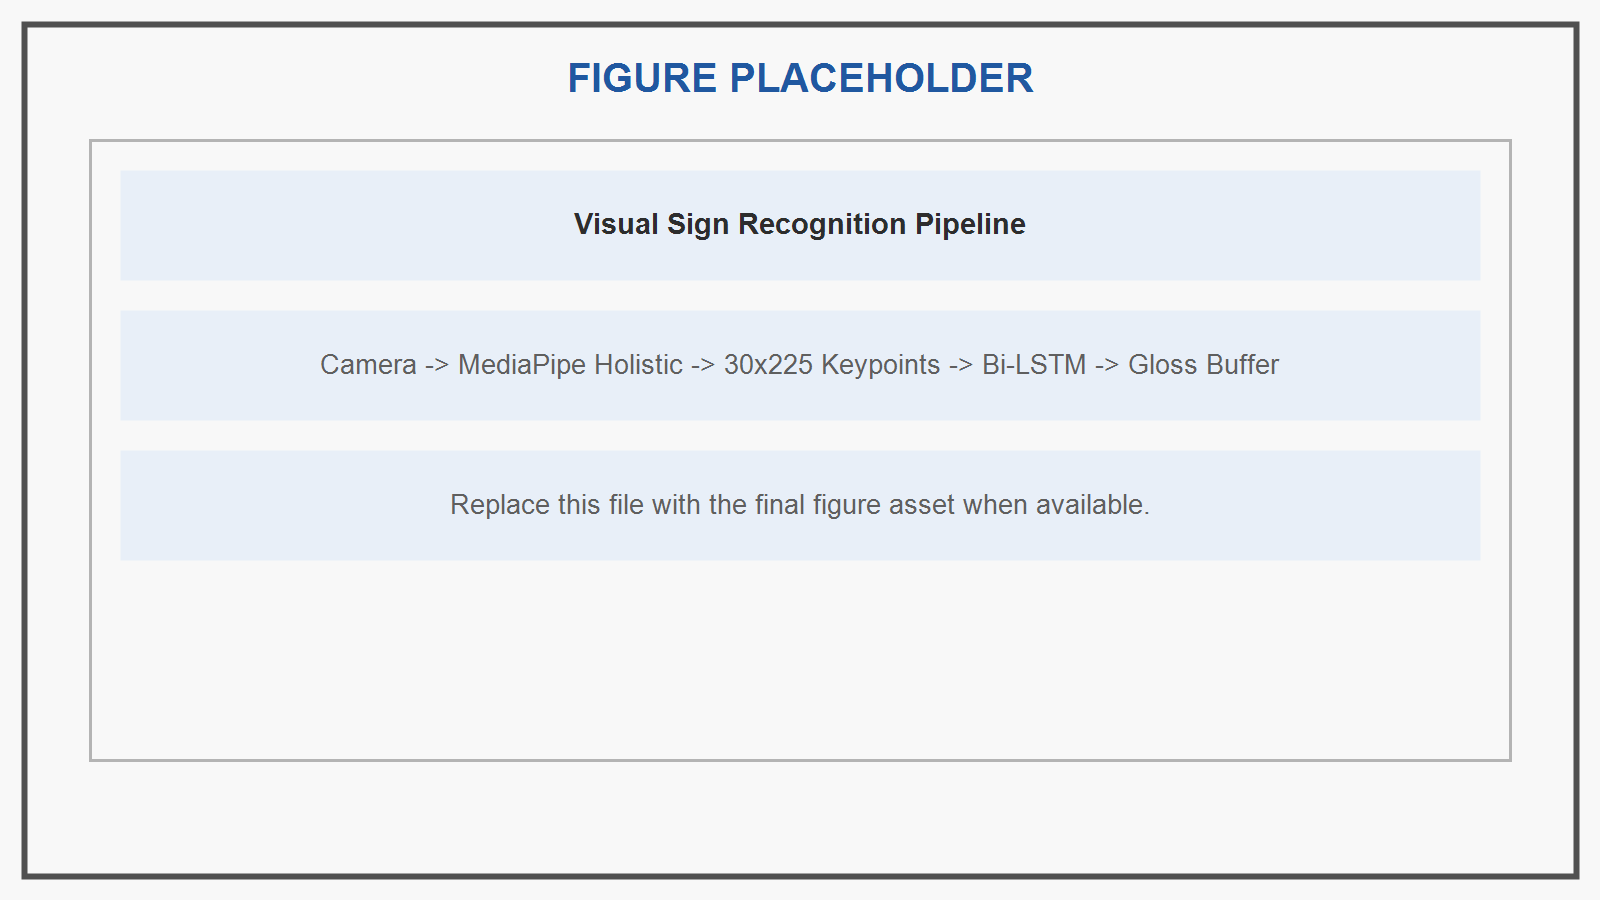
\includegraphics[width=0.88\textwidth]{figures/recognition/vsl_recognition_pipeline.png}
\caption{Vị trí của mô-đun nhận diện thị giác trong pipeline tổng thể}
\label{fig:vsl-recognition-pipeline}
\end{figure}

\subsubsection{Phát biểu bài toán}

Xét một đoạn video ngắn hoặc một cửa sổ trượt gồm nhiều frame liên tiếp từ webcam, mục tiêu của mô
hình là dự đoán ra một nhãn từ vựng ký hiệu tương ứng. Trong dự án này, đầu ra của mô hình là một
\textit{gloss} ở mức từ hoặc cụm từ ngắn, ví dụ \texttt{drink}, \texttt{hello}, \texttt{help},
\texttt{food}. Gloss đó sau đó có thể được ánh xạ sang token tiếng Việt tương ứng.

Do ký hiệu là tín hiệu có tính động, bài toán không thể chỉ nhìn một frame đơn lẻ. Ý nghĩa của một
từ ký hiệu thường phụ thuộc đồng thời vào:
\begin{itemize}
    \item vị trí tương đối giữa tay, vai, khuỷu tay và thân người;
    \item hình dạng và quỹ đạo chuyển động của hai bàn tay;
    \item biểu cảm khuôn mặt và hướng nhìn;
    \item thứ tự diễn tiến của các động tác theo thời gian.
\end{itemize}

Vì vậy, mô hình được thiết kế như một bộ phân loại đa lớp trên \textit{chuỗi đặc trưng theo thời
gian}, thay vì trên từng ảnh tĩnh.

\subsubsection{Vai trò của MediaPipe Holistic trong pipeline}

Theo tài liệu chính thức của Google, MediaPipe Holistic có thể xuất tổng cộng 543 landmarks trong
thời gian thực, bao gồm 468 điểm khuôn mặt, 33 điểm pose và 21 điểm cho mỗi bàn tay. Khác với
phiên bản trước của dự án (chỉ dùng pose và bàn tay với 225 đặc trưng), mô hình hiện tại giữ lại
\textbf{toàn bộ 543 landmarks} để tận dụng tối đa thông tin về biểu cảm khuôn mặt, thân trên và
hai bàn tay. Đây là lựa chọn phù hợp vì:
\begin{itemize}
    \item mô hình TFLite đã được huấn luyện trên toàn bộ 543 landmarks, nên đầu vào phải giữ nguyên
    cấu trúc này;
    \item landmarks khuôn mặt bổ sung thêm tín hiệu biểu cảm quan trọng cho nhiều từ ký hiệu;
    \item MediaPipe Holistic đã được tối ưu cho luồng ảnh liên tục, phù hợp với bài toán realtime
    trên webcam.
\end{itemize}

\begin{figure}[H]
\centering
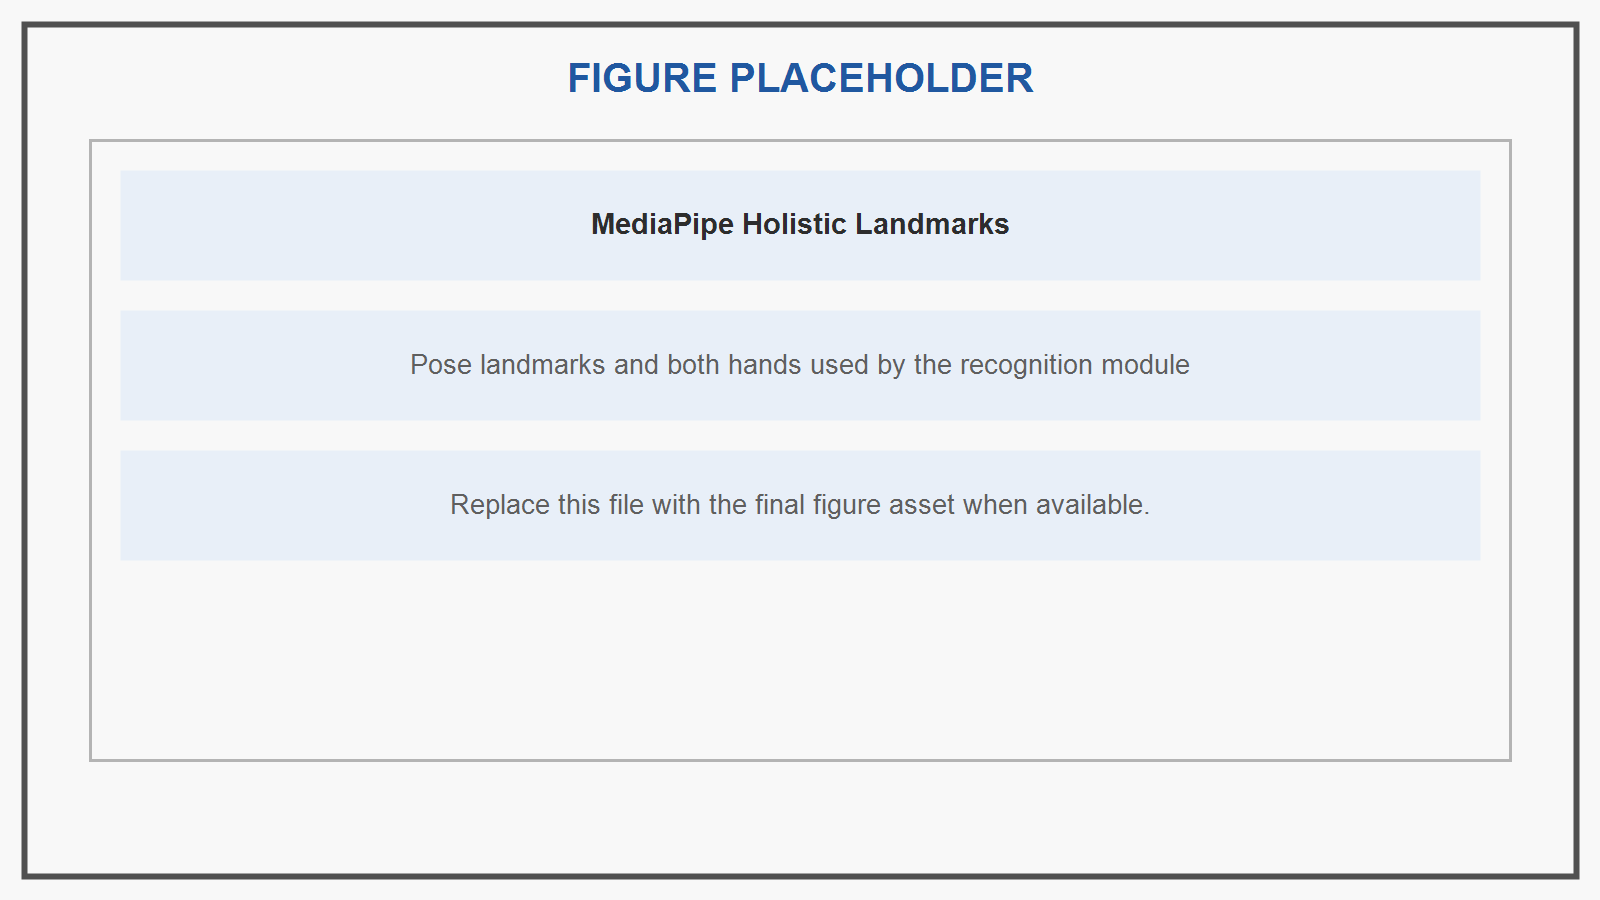
\includegraphics[width=0.84\textwidth]{figures/recognition/mediapipe_holistic_landmarks.png}
\caption{Minh họa landmarks pose, khuôn mặt và bàn tay được trích xuất bởi MediaPipe Holistic}
\label{fig:mediapipe-holistic-landmarks}
\end{figure}

\begin{table}[H]
\centering
\caption{Thành phần vector đặc trưng ở mỗi frame}
\label{tab:recognition-feature-layout}
\begin{tabularx}{\textwidth}{|p{3.4cm}|c|c|c|}
\hline
\textbf{Thành phần} & \textbf{Số điểm} & \textbf{Số tọa độ/điểm} & \textbf{Tổng đặc trưng} \\
\hline
Khuôn mặt & 468 & 3 & 1.404 \\
\hline
Tay trái & 21 & 3 & 63 \\
\hline
Pose & 33 & 3 & 99 \\
\hline
Tay phải & 21 & 3 & 63 \\
\hline
\textbf{Tổng} & \textbf{543} & \textbf{3} & \textbf{1.629} \\
\hline
\end{tabularx}
\end{table}

\subsubsection{Biểu diễn đầu vào theo chuỗi landmarks}

Sau khi một frame được biến thành ma trận landmarks kích thước \texttt{543 x 3}, hệ thống gom
các frame liên tiếp thành một chuỗi có độ dài linh hoạt. Trong code hiện tại
(\texttt{realtime\_asl\_250.py}), cửa sổ trượt có kích thước tối đa 60 frame và yêu cầu tối thiểu
16 frame trước khi bắt đầu suy luận. Kết quả là mỗi lần suy luận nhận đầu vào là một tensor
kích thước \texttt{N x 543 x 3}, với \texttt{N} nằm trong khoảng \texttt{[16, 60]}.

Điểm khác biệt quan trọng so với các thiết kế chuỗi cố định là mô hình TFLite có khả năng nhận
đầu vào có chiều dài thay đổi nhờ cơ chế \texttt{resize\_tensor\_input()}. Điều này mang lại hai
lợi ích:
\begin{itemize}
    \item mô hình có thể bắt đầu dự đoán sớm ngay khi có đủ 16 frame, giảm độ trễ ban đầu;
    \item khi cửa sổ trượt đầy (60 frame), mô hình có nhiều ngữ cảnh hơn để phân loại chính xác.
\end{itemize}

Một chi tiết kỹ thuật quan trọng trong code là nếu frame bị mất landmark, hệ thống sẽ đệm bằng
\texttt{NaN} thay vì vector zero. Đây là quy ước của mô hình Kaggle ASL Signs: giá trị \texttt{NaN}
cho phép mô hình phân biệt giữa ``không có tay'' và ``tay ở vị trí gốc tọa độ''.

\begin{figure}[H]
\centering
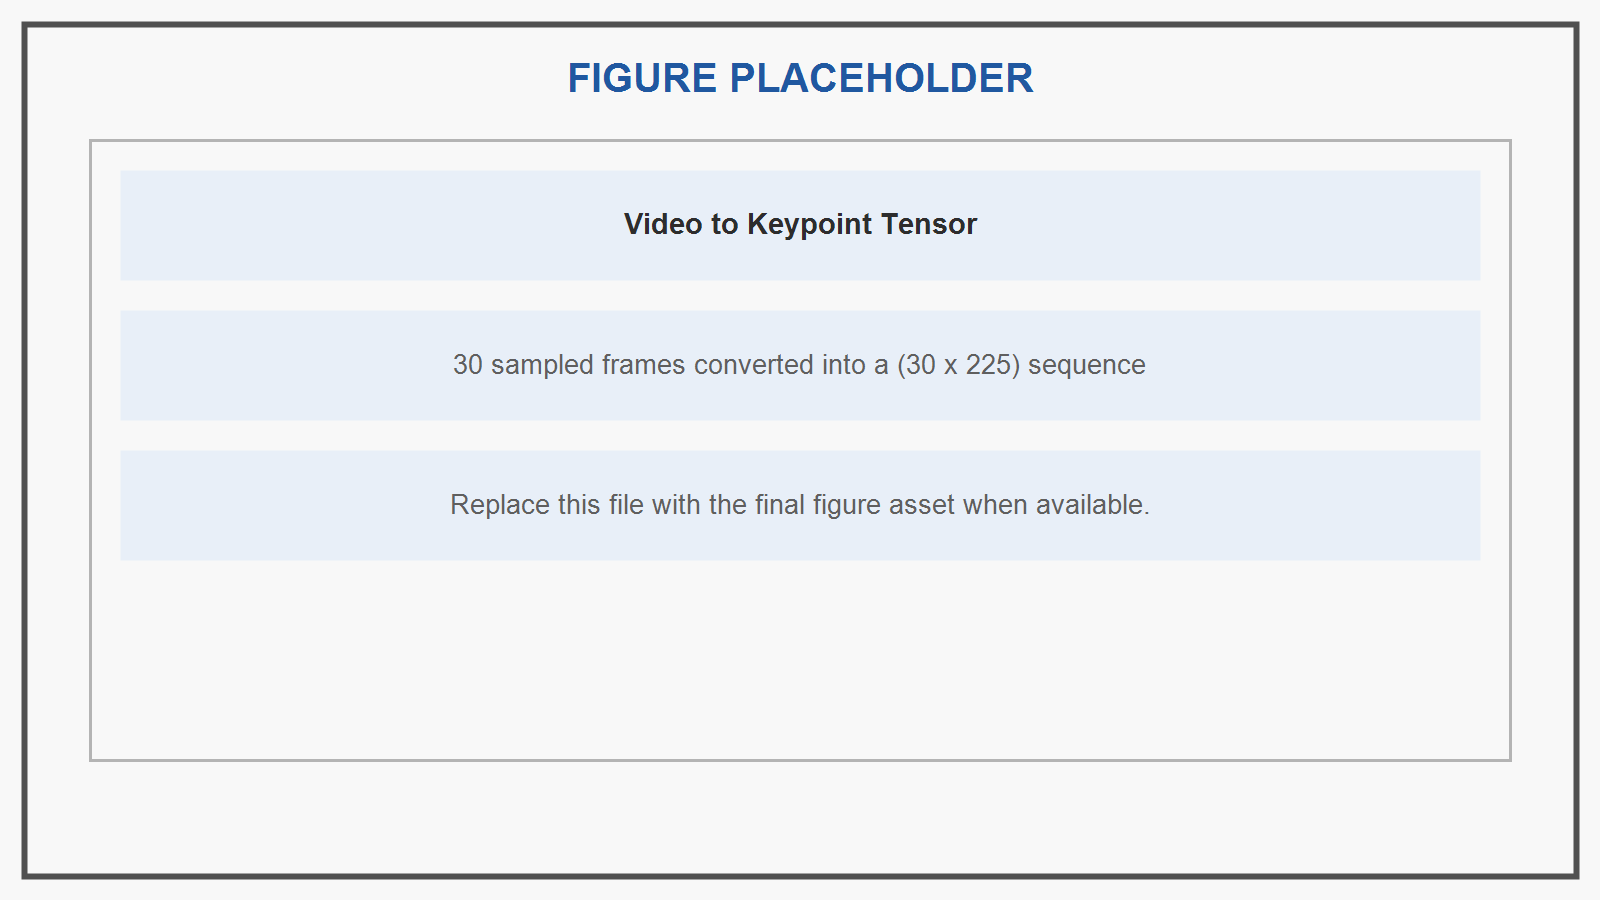
\includegraphics[width=0.82\textwidth]{figures/recognition/keypoint_vectorization.png}
\caption{Sơ đồ biến video thành chuỗi landmarks kích thước N x 543 x 3}
\label{fig:keypoint-vectorization}
\end{figure}

\subsubsection{Kiến trúc mô hình TFLite (Kaggle ASL Signs 1st Place)}

Mô hình nhận diện trong dự án là giải pháp đạt giải nhất cuộc thi
\textit{Google -- Isolated Sign Language Recognition} trên Kaggle. Mô hình đã được chuyển đổi
sang định dạng TensorFlow Lite (\texttt{model.tflite}) để tối ưu cho suy luận nhanh trên thiết
bị đầu cuối.

Về kiến trúc, mô hình này khác biệt hoàn toàn so với các mạng hồi quy truyền thống:
\begin{itemize}
    \item đầu vào là chuỗi landmarks có chiều dài linh hoạt, mỗi frame gồm 543 điểm x 3 tọa độ;
    \item mô hình được huấn luyện end-to-end trên dữ liệu landmarks, không cần bước trích xuất
    đặc trưng thủ công;
    \item đầu ra là phân bố xác suất trên 250 lớp từ vựng ký hiệu ASL;
    \item mô hình sử dụng TFLite Interpreter cho suy luận, cho phép chạy trên CPU mà không cần GPU.
\end{itemize}

Trong code, quá trình suy luận được thực hiện qua các bước:
\begin{enumerate}
    \item gom landmarks thành tensor đầu vào;
    \item gọi \texttt{interpreter.resize\_tensor\_input()} để điều chỉnh kích thước đầu vào
    theo số frame thực tế;
    \item gọi \texttt{interpreter.allocate\_tensors()} và \texttt{set\_tensor()};
    \item gọi \texttt{interpreter.invoke()} để chạy suy luận;
    \item lấy kết quả từ \texttt{get\_tensor()}, áp dụng softmax nếu cần;
    \item chọn top-k lớp có xác suất cao nhất.
\end{enumerate}

File \texttt{sign\_to\_prediction\_index\_map.json} chứa bảng ánh xạ giữa tên từ vựng ký hiệu
và chỉ số đầu ra của mô hình, cho phép chuyển đổi kết quả số thành nhãn có nghĩa.

\begin{table}[H]
\centering
\caption{Thông số chính của mô hình nhận diện}
\label{tab:recognition-hyperparameters}
\begin{tabularx}{\textwidth}{|p{5cm}|X|}
\hline
\textbf{Tham số} & \textbf{Giá trị trong code} \\
\hline
Số lớp từ vựng & 250 \\
\hline
Kích thước đầu vào mỗi frame & 543 landmarks x 3 tọa độ \\
\hline
Số frame tối thiểu & 16 \\
\hline
Số frame tối đa (sliding window) & 60 \\
\hline
Tần suất suy luận & Mỗi 8 frame \\
\hline
Top-k hiển thị & 3 \\
\hline
Định dạng mô hình & TensorFlow Lite (.tflite) \\
\hline
Kích thước file mô hình & $\sim$11 MB \\
\hline
\end{tabularx}
\end{table}

\subsubsection{Nguồn gốc mô hình và dữ liệu huấn luyện}

Mô hình TFLite được lấy từ giải pháp đạt giải nhất cuộc thi Kaggle
\textit{Google -- Isolated Sign Language Recognition}. Cuộc thi này yêu cầu các đội thi xây
dựng mô hình nhận diện 250 từ vựng ký hiệu ASL từ dữ liệu landmarks đã được trích xuất
bằng MediaPipe Holistic.

Dữ liệu huấn luyện gốc của cuộc thi bao gồm:
\begin{itemize}
    \item 250 từ vựng ký hiệu ASL phổ biến;
    \item dữ liệu landmarks đã được trích xuất sẵn (không phải video RGB);
    \item nhiều signer với điều kiện ghi hình khác nhau.
\end{itemize}

Vì đây là mô hình pre-trained, nhóm không thực hiện quá trình huấn luyện lại. Thay vào đó,
mô hình được sử dụng trực tiếp làm thành phần nhận diện trong pipeline tổng thể. Đây là một
lựa chọn thực dụng cho đồ án vì cho phép tập trung nguồn lực vào các tầng NLP phía sau,
đồng thời vẫn đảm bảo chất lượng nhận diện ở mức cạnh tranh nhờ vào kết quả đã được kiểm
chứng qua cuộc thi.

\subsubsection{Cơ chế suy luận thời gian thực}

Trong \texttt{realtime\_asl\_250.py}, hệ thống duy trì một bộ đệm trượt:
\begin{itemize}
    \item \texttt{frames = deque(maxlen=60)};
    \item chỉ gom frame khi phát hiện có bàn tay (trái hoặc phải) xuất hiện trong khung hình;
    \item suy luận mỗi 8 frame (\texttt{predict\_every=8});
    \item chỉ bắt đầu suy luận khi bộ đệm đủ tối thiểu 16 frame;
    \item hiển thị top-3 dự đoán có xác suất cao nhất;
    \item nhấn phím Space để reset bộ đệm, phím \texttt{q} để thoát.
\end{itemize}

Thiết kế ``chỉ gom khi có tay'' là một cải tiến quan trọng: thay vì gom mọi frame kể cả khi
người dùng không ký hiệu, hệ thống chỉ thu thập dữ liệu khi phát hiện ít nhất một bàn tay.
Điều này giúp giảm nhiễu đầu vào và tăng chất lượng dự đoán.

\subsubsection{Ưu điểm và giới hạn của thiết kế hiện tại}

Thiết kế \textit{MediaPipe Holistic + TFLite pre-trained} có một số ưu điểm rõ ràng:
\begin{itemize}
    \item mô hình đã được kiểm chứng qua cuộc thi Kaggle với chất lượng cao;
    \item sử dụng toàn bộ 543 landmarks bao gồm cả biểu cảm khuôn mặt;
    \item kiến trúc gọn, suy luận bằng TFLite trên CPU, phù hợp với phần cứng phổ thông;
    \item cửa sổ trượt linh hoạt 16--60 frame và logic ``chỉ gom khi có tay'' phù hợp cho
    demo realtime;
    \item đầu ra gloss là giao diện trung gian thuận lợi để nối với tầng NLP.
\end{itemize}

Mặt khác, vẫn còn các giới hạn quan trọng:
\begin{itemize}
    \item mô hình được huấn luyện trên dữ liệu ASL, không phải VSL gốc, nên tính đúng đắn
    ngôn ngữ còn phụ thuộc bước ánh xạ gloss;
    \item số lớp từ vựng là 250, ít hơn so với nhu cầu giao tiếp thực tế;
    \item mô hình hiện nhận diện ở mức từ đơn lẻ, chưa xử lý trực tiếp câu ký hiệu liên tục;
    \item vì là mô hình pre-trained, nhóm không thể can thiệp vào kiến trúc bên trong hoặc
    tinh chỉnh cho VSL;
    \item chất lượng cuối cùng của pipeline chịu ảnh hưởng mạnh từ ánh sáng, góc quay, che khuất
    tay và sự khác biệt giữa signer thật với signer trong dữ liệu Kaggle.
\end{itemize}


\subsection{Mô hình ghép từ thành câu tiếng Việt}

Sau khi tầng nhận diện ký hiệu dự đoán ra các gloss hoặc cụm gloss theo thời gian, hệ
thống vẫn chưa thể giao tiếp trực tiếp với người dùng cuối. Chuỗi đầu ra ở giai đoạn này
thường chỉ là các đơn vị ý nghĩa rời rạc như \texttt{toi muon uong\_nuoc},
\texttt{toi can giup\_do} hoặc \texttt{toi dau bung}. Vì vậy, cần có một mô-đun xử lý ngôn
ngữ tự nhiên để tái cấu trúc chuỗi đó thành câu tiếng Việt hoàn chỉnh, có chủ ngữ, vị ngữ,
dấu câu và cách diễn đạt tự nhiên hơn.

Về bản chất, đây là bài toán \textit{sequence-to-sequence}: đầu vào là chuỗi gloss đã được
chuẩn hóa, đầu ra là câu tiếng Việt hoàn chỉnh. Trong các nghiên cứu gần đây về dịch ngôn
ngữ ký hiệu, pha \textit{Gloss-to-Text} vẫn được xem là một bước quan trọng để nối tầng
thị giác với tầng sinh ngôn ngữ, và thường được đánh giá bằng các metric như BLEU,
ROUGE hoặc chrF. Trong đồ án này, thay vì dùng trực tiếp một mô hình đa ngôn ngữ,
nhóm lựa chọn một mô hình sinh văn bản đơn ngữ dành riêng cho tiếng Việt để tối ưu chất
lượng diễn đạt ở ngôn ngữ đích.

\begin{figure}[H]
\centering
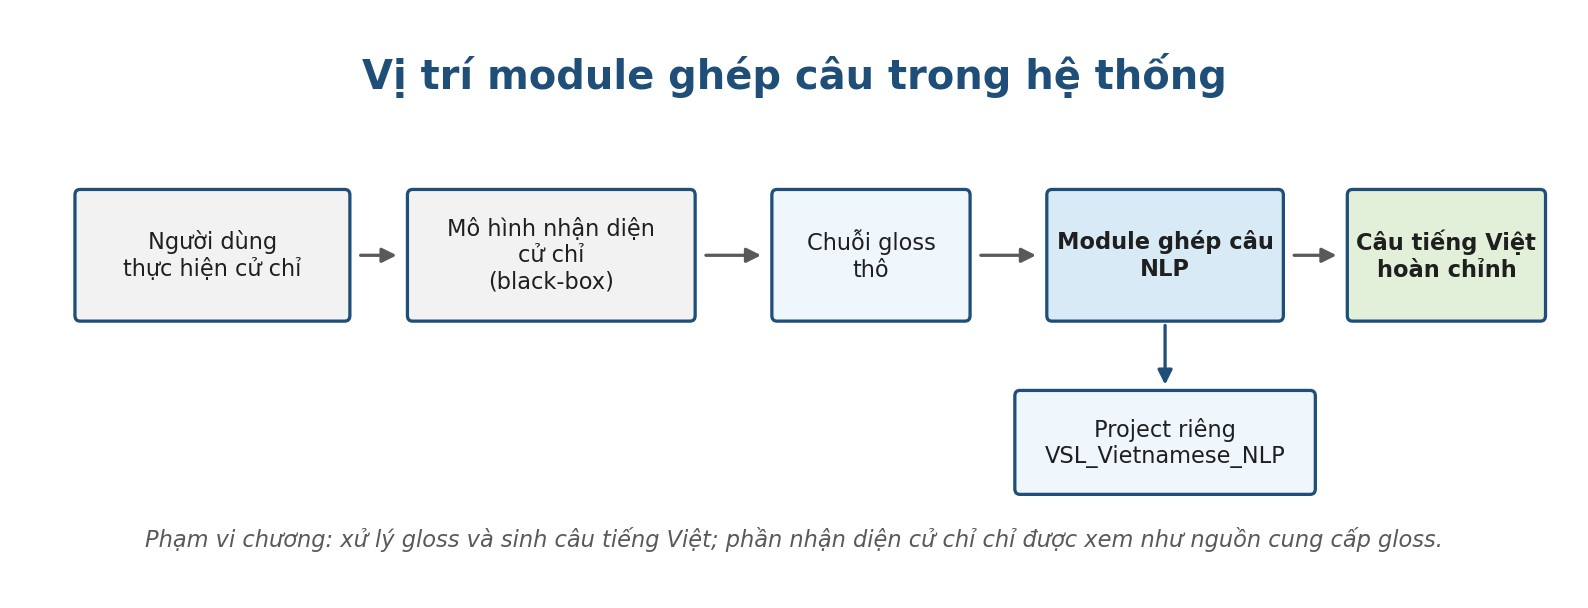
\includegraphics[width=0.95\textwidth]{figures/nlp/vsl_module_position.jpg}
\caption{Vị trí của mô-đun ghép câu trong hệ thống xử lý ký hiệu}
\label{fig:gloss-to-sentence-pipeline}
\end{figure}

\subsubsection{Phát biểu bài toán}

Cho một chuỗi gloss đầu vào nhận được từ tầng nhận diện ký hiệu, mô-đun ghép câu cần
sinh ra một chuỗi đầu ra là câu tiếng Việt hoàn chỉnh sao cho:
\begin{itemize}
    \item bảo toàn ý nghĩa cốt lõi của chuỗi gloss đầu vào;
    \item bổ sung được các thành phần ngữ pháp cần thiết cho tiếng Việt;
    \item giảm tính rời rạc, lặp từ và thiếu dấu câu của đầu ra trung gian;
    \item đủ nhẹ để tích hợp vào chế độ realtime.
\end{itemize}

Ví dụ, chuỗi \texttt{toi muon uong\_nuoc} không nên chỉ được hiển thị nguyên dạng, mà
cần được chuyển thành câu \textit{Tôi muốn uống nước.} Tương tự,
\texttt{toi can giup\_do} nên được chuyển thành \textit{Tôi cần giúp đỡ.}

\subsubsection{Kiến trúc lai được sử dụng}

Thay vì phụ thuộc hoàn toàn vào một mô hình sinh văn bản, project hiện thực mô-đun này
theo kiến trúc lai gồm ba tầng ưu tiên:
\begin{enumerate}
    \item \textbf{Rule-based/template}: tra cứu các mẫu câu có tần suất cao trong
    \codepath{configs/sentence_rules.json}. Đây là tầng có độ ổn định cao nhất và phản hồi
    rất nhanh.
    \item \textbf{BARTpho fine-tuned}: nếu chuỗi đầu vào không khớp rule cứng, hệ thống
    dùng mô hình sinh văn bản để phục hồi câu tiếng Việt linh hoạt hơn.
    \item \textbf{Fallback corrector}: nếu mô hình chưa được huấn luyện hoặc không thể
    nạp, hệ thống vẫn còn tầng dự phòng để ánh xạ token cơ bản và thêm dấu câu tối thiểu.
\end{enumerate}

Thiết kế này bám sát hiện thực trong mã nguồn: lớp \texttt{SentenceBuilder} lần lượt kiểm
tra rule, gọi predictor BARTpho và cuối cùng rơi về tầng fallback. Cách tổ chức như vậy giúp mô-đun vừa có khả năng sinh câu
tự nhiên, vừa đảm bảo tính an toàn khi triển khai thực tế.

\begin{figure}[H]
\centering
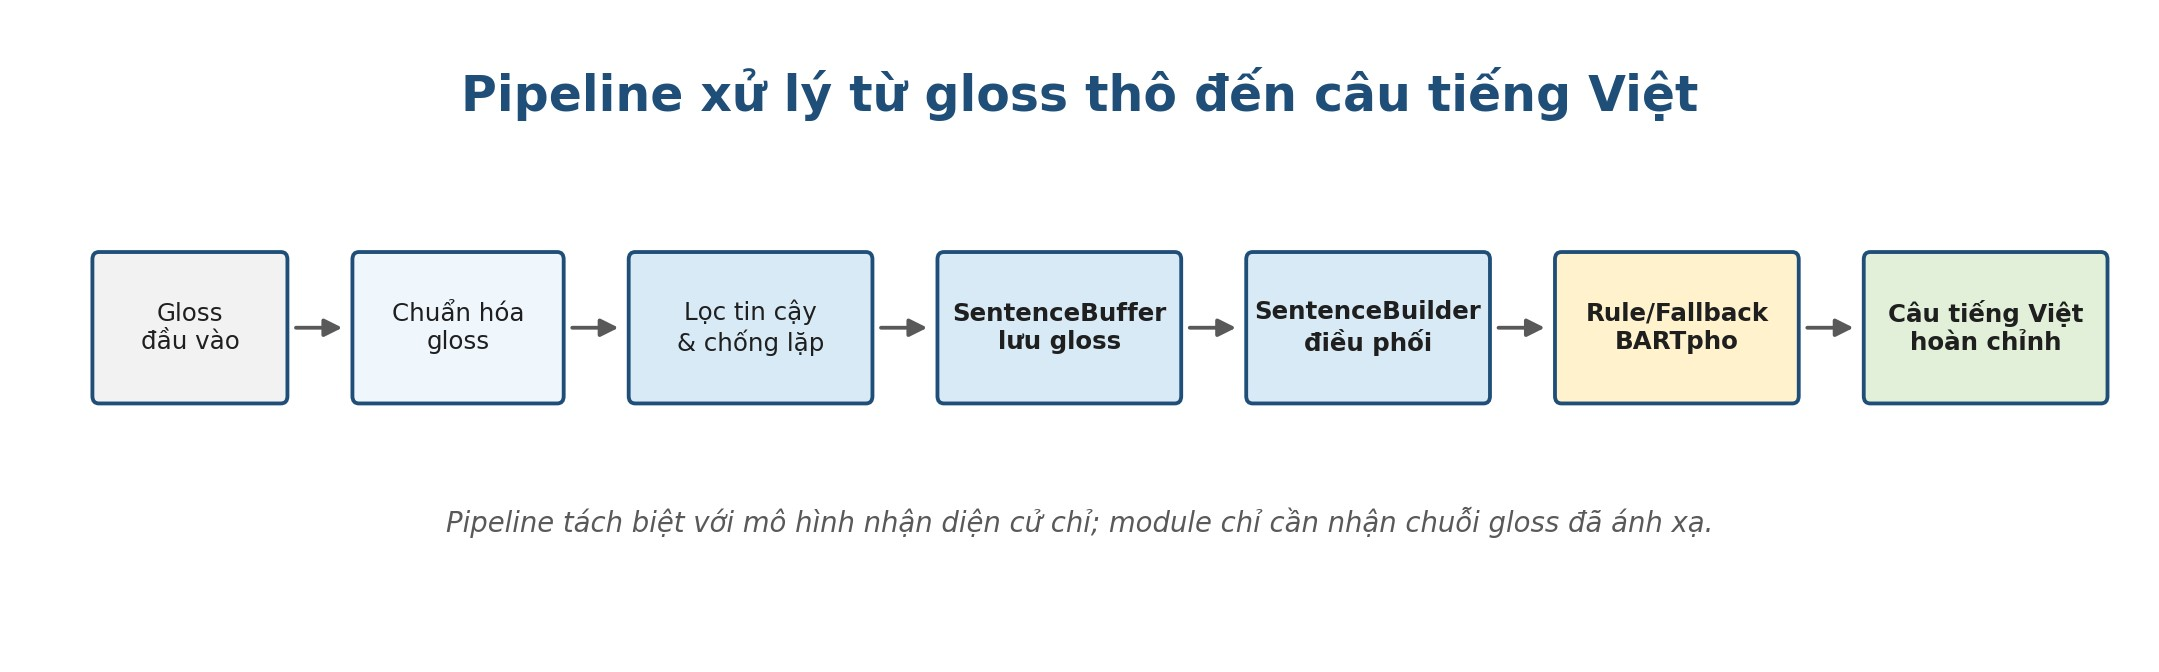
\includegraphics[width=0.95\textwidth]{figures/nlp/vsl_gloss_processing_pipeline.jpg}
\caption{Pipeline xử lý từ gloss thô đến câu tiếng Việt hoàn chỉnh}
\label{fig:vsl-gloss-processing-pipeline}
\end{figure}

\begin{figure}[H]
\centering
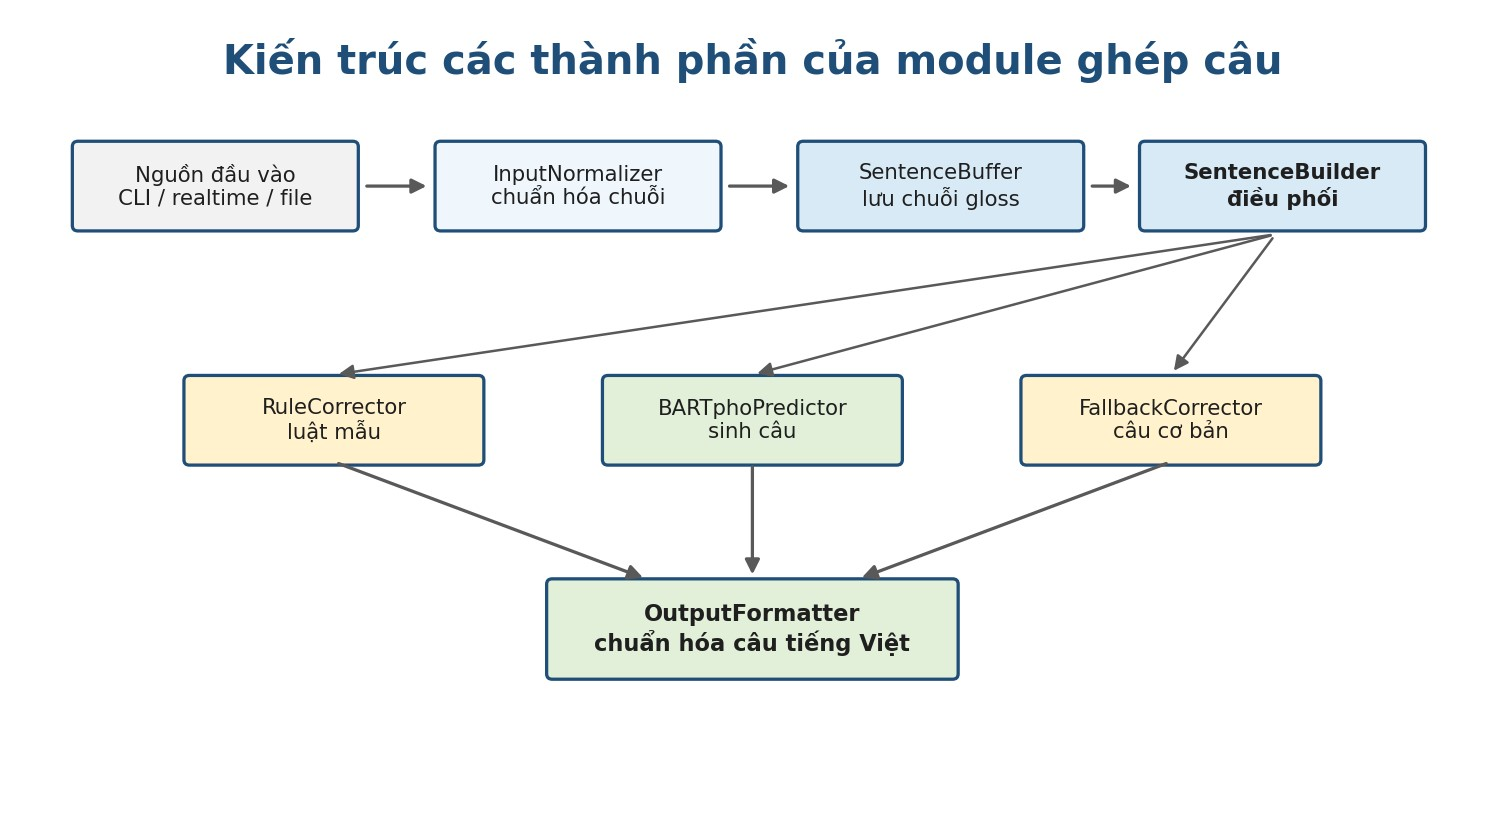
\includegraphics[width=0.9\textwidth]{figures/nlp/vsl_sentence_module_architecture.jpg}
\caption{Kiến trúc các thành phần chính của mô-đun ghép câu}
\label{fig:hybrid-sentence-builder}
\end{figure}

\begin{table}[H]
\centering
\caption{Vai trò của các thành phần trong mô-đun ghép câu}
\begin{tabularx}{\textwidth}{|p{3.2cm}|X|X|}
\hline
\textbf{Thành phần} & \textbf{Vai trò chính} & \textbf{Ý nghĩa trong hệ thống realtime} \\
\hline
Rule/template & Xử lý các mẫu giao tiếp ngắn, lặp lại nhiều lần như chào hỏi, xin lỗi, yêu cầu hỗ trợ. & Phản hồi gần như tức thời, giảm phụ thuộc vào mô hình sinh. \\
\hline
BARTpho fine-tuned & Khôi phục câu tự nhiên cho các chuỗi gloss linh hoạt hoặc chưa có rule. & Tăng độ tự nhiên và khả năng tổng quát hóa của đầu ra. \\
\hline
Fallback corrector & Ánh xạ token cơ bản, viết hoa đầu câu và thêm dấu câu tối thiểu. & Đảm bảo hệ thống vẫn sử dụng được khi mô hình chưa sẵn sàng. \\
\hline
\end{tabularx}
\end{table}

\subsubsection{Lý do chọn BARTpho}

BARTpho là mô hình \textit{sequence-to-sequence} đơn ngữ đầu tiên được tiền huấn luyện
quy mô lớn cho tiếng Việt. Theo Tran, Le và Nguyen, BARTpho có hai biến thể là
\textit{BARTpho-syllable} và \textit{BARTpho-word}; mô hình sử dụng kiến trúc
\textit{BART-large} và đặc biệt phù hợp với các tác vụ sinh văn bản tiếng Việt. Về gốc,
BART là một \textit{denoising autoencoder} kết hợp encoder hai chiều và decoder sinh
trái sang phải, nhờ đó rất phù hợp cho các tác vụ phục hồi câu, tóm tắt hoặc tái cấu trúc
chuỗi.

Trong project này, cấu hình \codepath{configs/nlp_config.json} chọn mô hình nền BARTpho word-base. Đây là lựa chọn hợp lý vì:
\begin{itemize}
    \item đầu vào của mô-đun đã ở dạng token từ hoặc cụm từ phân cách bằng khoảng
    trắng;
    \item nhiều gloss dùng dấu gạch dưới để biểu diễn cụm từ cố định như
    \texttt{uong\_nuoc}, \texttt{benh\_vien}, \texttt{giup\_do};
    \item mô hình đơn ngữ tiếng Việt thường diễn đạt câu đích mượt hơn so với mô hình đa
    ngôn ngữ tổng quát khi tác vụ chỉ có một ngôn ngữ đầu ra.
\end{itemize}

Để đồng nhất giữa huấn luyện và suy luận, project thêm tiền tố nhiệm vụ \codepath{chuyen_cau_ky_hieu:}
vào chuỗi đầu vào trước khi token hóa. Đây là một chi tiết
quan trọng vì giúp mô hình hiểu đúng ngữ cảnh nhiệm vụ sinh câu, đồng thời tránh lệch
phân phối giữa train và inference.

\begin{figure}[H]
\centering
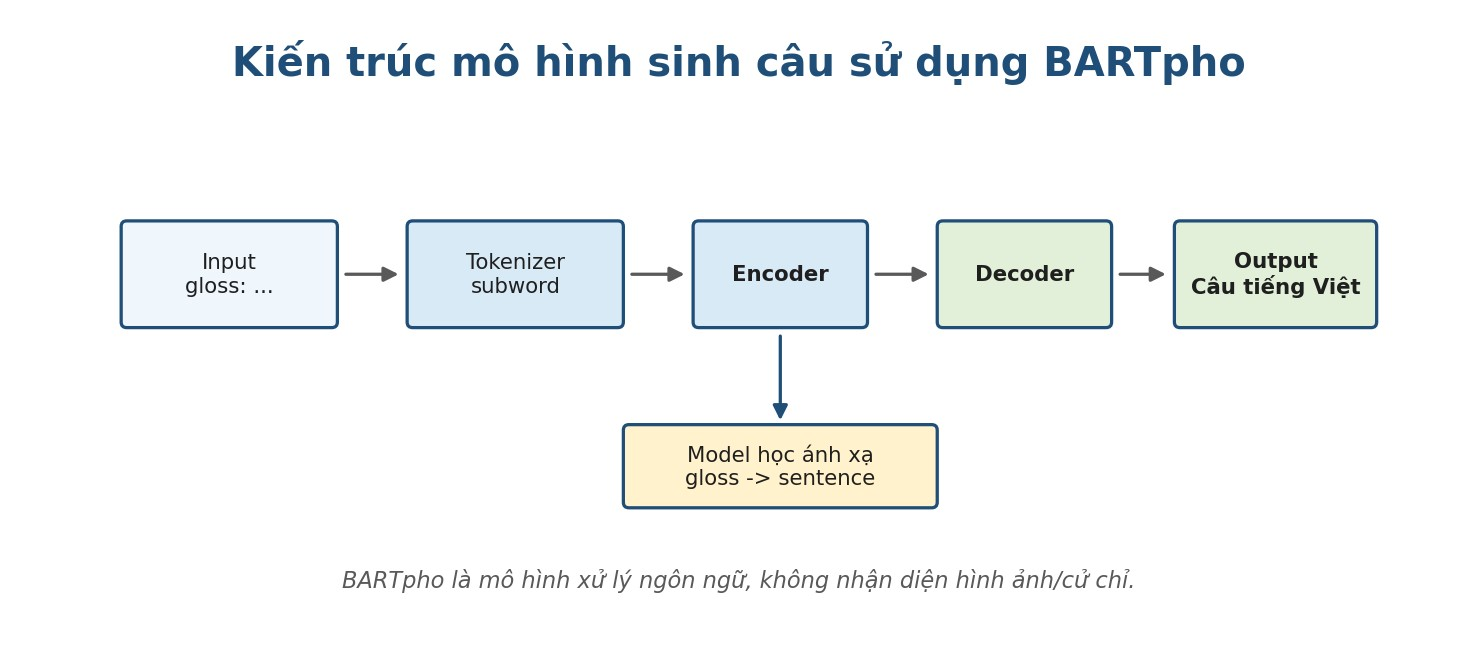
\includegraphics[width=0.88\textwidth]{figures/nlp/vsl_bartpho_generation_architecture.jpg}
\caption{Kiến trúc sinh câu tiếng Việt bằng BARTpho}
\label{fig:bartpho-architecture}
\end{figure}

\subsubsection{Thông số thiết kế chính}

Các thông số nổi bật đang được dùng trong project gồm:
\begin{itemize}
    \item mô hình nền: \texttt{vinai/bartpho-word-base};
    \item độ dài tối đa đầu vào: 64 token;
    \item độ dài tối đa đầu ra: 64 token;
    \item huấn luyện với \texttt{AdamW}, learning rate \texttt{5e-5};
    \item suy luận dùng \texttt{beam search} với \texttt{num\_beams = 4}.
\end{itemize}

Bên cạnh cấu hình suy luận/demo đang lưu trong repository, tài liệu \texttt{vsl.pdf} ghi nhận
lần fine-tune chính của BARTpho được thực hiện trên Google Colab với cấu hình dài hơn cho
chuỗi nguồn và chuỗi đích. Cấu hình này được dùng làm căn cứ cho phần đánh giá ở
Chương~4.

\begin{table}[H]
\centering
\caption{Cấu hình fine-tune BARTpho}
\label{tab:bartpho-finetune-config-vsl}
\begin{tabularx}{0.86\textwidth}{|X|c|}
\hline
\textbf{Thành phần} & \textbf{Giá trị} \\
\hline
Môi trường & Google Colab \\
\hline
GPU & T4 \\
\hline
Mô hình gốc & BARTpho \\
\hline
Số epoch & 5 \\
\hline
Batch size & 4 \\
\hline
Max source length & 96 \\
\hline
Max target length & 128 \\
\hline
\end{tabularx}
\end{table}

\begin{figure}[H]
\centering
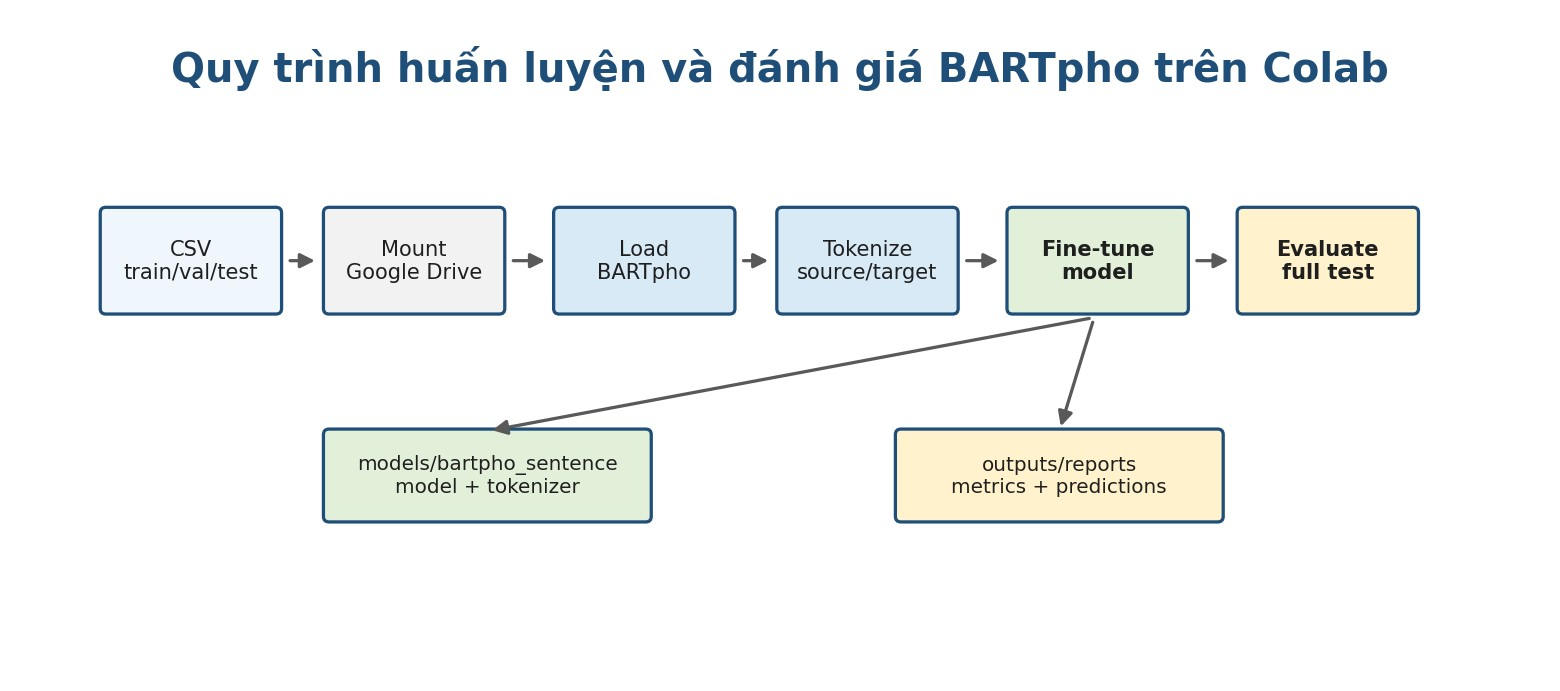
\includegraphics[width=0.9\textwidth]{figures/nlp/vsl_bartpho_training_evaluation_pipeline.jpg}
\caption{Quy trình huấn luyện và đánh giá BARTpho}
\label{fig:vsl-bartpho-training-evaluation-pipeline}
\end{figure}

Tập luật hiện tại đóng vai trò như một lớp tri thức miền hẹp, đặc biệt hữu ích với các câu
giao tiếp chăm sóc sức khỏe hoặc nhu cầu cơ bản. Khi gloss đầu vào chưa có trong tập
luật, BARTpho đảm nhiệm phần tổng quát hóa. Nếu cả hai đường này đều không khả dụng,
fallback sẽ duy trì đầu ra đọc được thay vì làm hỏng toàn bộ pipeline.

\subsubsection{Ưu điểm và giới hạn}

Ưu điểm lớn nhất của kiến trúc hiện tại là cân bằng giữa \textit{độ ổn định} và
\textit{độ tự nhiên}. Rule-based giúp giữ đúng các mẫu câu quan trọng, còn BARTpho cho
phép mô-đun không bị giới hạn ở một tập câu cứng. Điều này đặc biệt phù hợp với hệ
thống thời gian thực, nơi lỗi của tầng nhận diện trước đó có thể lan sang tầng NLP.

Tuy nhiên, mô-đun này vẫn có một số giới hạn:
\begin{itemize}
    \item nếu chuỗi gloss đầu vào sai quá nhiều do nhận diện nhầm, mô hình sinh câu vẫn có
    thể bảo toàn lỗi ngữ nghĩa;
    \item tập luật hiện tại phù hợp nhất với miền giao tiếp cơ bản, chưa đủ bao phủ hội thoại
    mở;
    \item chất lượng metric rất cao trên bộ dữ liệu sinh theo template không đồng nghĩa với
    khả năng tổng quát hóa hoàn toàn ngoài miền dữ liệu đó.
\end{itemize}


\subsection{Mô hình dịch Việt - Lào}

Tầng thứ ba của hệ thống nhận câu tiếng Việt đã được chuẩn hóa từ mô-đun trước và dịch
sang tiếng Lào. Nếu mô-đun ghép câu giúp đầu ra trở nên tự nhiên trong nội ngữ, thì mô
đun này mở rộng hệ thống sang giao tiếp liên ngôn ngữ. Trong bối cảnh của đồ án, đây là
khâu biến một pipeline nhận diện ký hiệu thành một pipeline truyền đạt thông tin cho người
dùng ở ngôn ngữ khác.

Tài liệu mô tả ban đầu trong \texttt{vilo.pdf} trình bày các khái niệm nền như
\textit{Sequence-to-Sequence}, \textit{Attention}, \textit{Transformer} và
\textit{Embedding}. Đối chiếu với mã nguồn thực tế, project hiện tại hiện thực hóa các ý
tưởng đó bằng mô hình NLLB-200 Distilled 600M kết hợp adapter LoRA, thay vì dùng một
kiến trúc Seq2Seq tự xây từ đầu.

\begin{figure}[H]
\centering
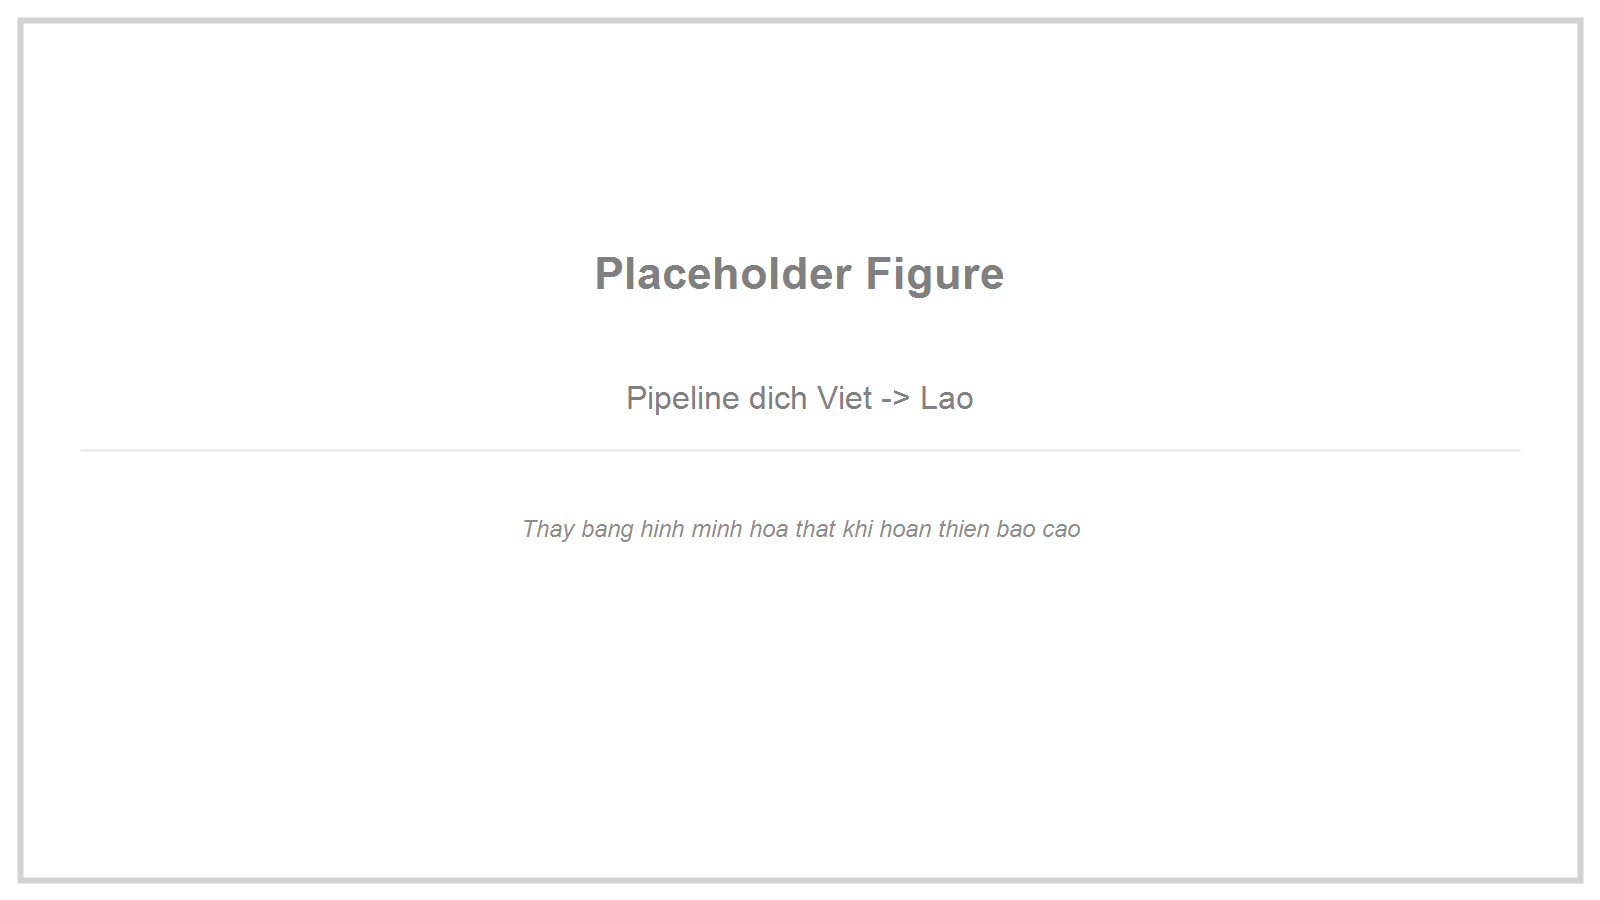
\includegraphics[width=0.88\textwidth]{figures/translation/vi_lao_mt_pipeline.png}
\caption{Vị trí của mô-đun dịch Việt - Lào trong pipeline tổng thể}
\label{fig:vi-lao-pipeline}
\end{figure}

\subsubsection{Bài toán dịch máy trong phạm vi đề tài}

Đầu vào của mô-đun là câu tiếng Việt đã qua tầng sửa ngữ pháp, ví dụ
\textit{Tôi muốn uống nước.} hoặc \textit{Tôi cần giúp đỡ.} Đầu ra mong muốn là câu
tiếng Lào tương đương về nghĩa, đủ tự nhiên để có thể hiển thị hoặc kết hợp với các tầng
hỗ trợ giao tiếp khác như text-to-speech.

Xét về mặt học máy, đây là bài toán dịch máy \textit{text-to-text}. Mô hình không chỉ cần
dịch đúng từ vựng, mà còn phải bảo toàn vai nghĩa, trật tự thông tin và cách dùng từ theo
đúng ngữ cảnh. Điều này đặc biệt quan trọng khi hệ thống phục vụ các tình huống giao
tiếp hỗ trợ, nơi một sai lệch nhỏ về nghĩa có thể làm thay đổi ý định của người dùng.

\subsubsection{Lý do chọn NLLB-200 Distilled 600M}

NLLB (\textit{No Language Left Behind}) là họ mô hình dịch máy đa ngôn ngữ do Meta
phát triển với mục tiêu hỗ trợ các ngôn ngữ tài nguyên thấp. Theo NLLB Team, công trình
này tập trung thu hẹp khoảng cách hiệu năng giữa ngôn ngữ giàu và nghèo tài nguyên, đồng
thời đánh giá trên hơn 40.000 hướng dịch và hướng tới mốc 200 ngôn ngữ. Với một
đề tài có cặp ngôn ngữ Việt - Lào, đây là một lựa chọn hợp lý vì tiếng Lào là ngôn ngữ ít
tài nguyên hơn nhiều so với các cặp dịch phổ biến như Anh - Pháp hoặc Anh - Đức.

Project sử dụng biến thể \texttt{nllb-200-distilled-600M}. So với các bản lớn hơn, bản
\textit{distilled 600M} cho phép:
\begin{itemize}
    \item giảm yêu cầu phần cứng, phù hợp hơn với môi trường triển khai học thuật;
    \item giữ được lợi thế của tiền huấn luyện đa ngôn ngữ;
    \item thuận tiện hơn khi tinh chỉnh bằng adapter thay vì full fine-tuning.
\end{itemize}

Vì đầu vào của mô-đun đã là câu tiếng Việt sạch ngữ pháp, NLLB đóng vai trò như một
khối dịch máy chuyên dụng nằm ở cuối pipeline, tận dụng kiến thức đa ngôn ngữ có sẵn
thay vì phải xây toàn bộ mô hình dịch mới từ đầu.

\subsubsection{Chiến lược tinh chỉnh bằng LoRA}

LoRA (\textit{Low-Rank Adaptation}) là kỹ thuật tinh chỉnh tham số hiệu quả, trong đó mô
hình gốc được giữ cố định và chỉ thêm các ma trận hạng thấp có khả năng học vào một số
lớp của Transformer. Theo Hu và cộng sự, cách làm này giúp giảm mạnh số tham số cần
cập nhật nhưng vẫn duy trì chất lượng tốt trên các tác vụ downstream.

Tệp \texttt{adapter\_config.json} trong project cho thấy adapter hiện tại có cấu hình:
\begin{itemize}
    \item \texttt{r = 16};
    \item \texttt{lora\_alpha = 32};
    \item \texttt{lora\_dropout = 0.05};
    \item áp dụng trên các module \texttt{q\_proj}, \texttt{k\_proj},
    \texttt{v\_proj} và \texttt{out\_proj};
    \item kiểu tác vụ: \texttt{SEQ\_2\_SEQ\_LM}.
\end{itemize}

Như vậy, project không huấn luyện lại toàn bộ NLLB mà chỉ học một lớp thích nghi mỏng
trên đỉnh mô hình nền. Đây là lựa chọn rất phù hợp với đồ án sinh viên vì vừa tiết kiệm tài
nguyên, vừa cho phép lưu trữ mô hình dưới dạng adapter nhỏ gọn.

\begin{figure}[H]
\centering
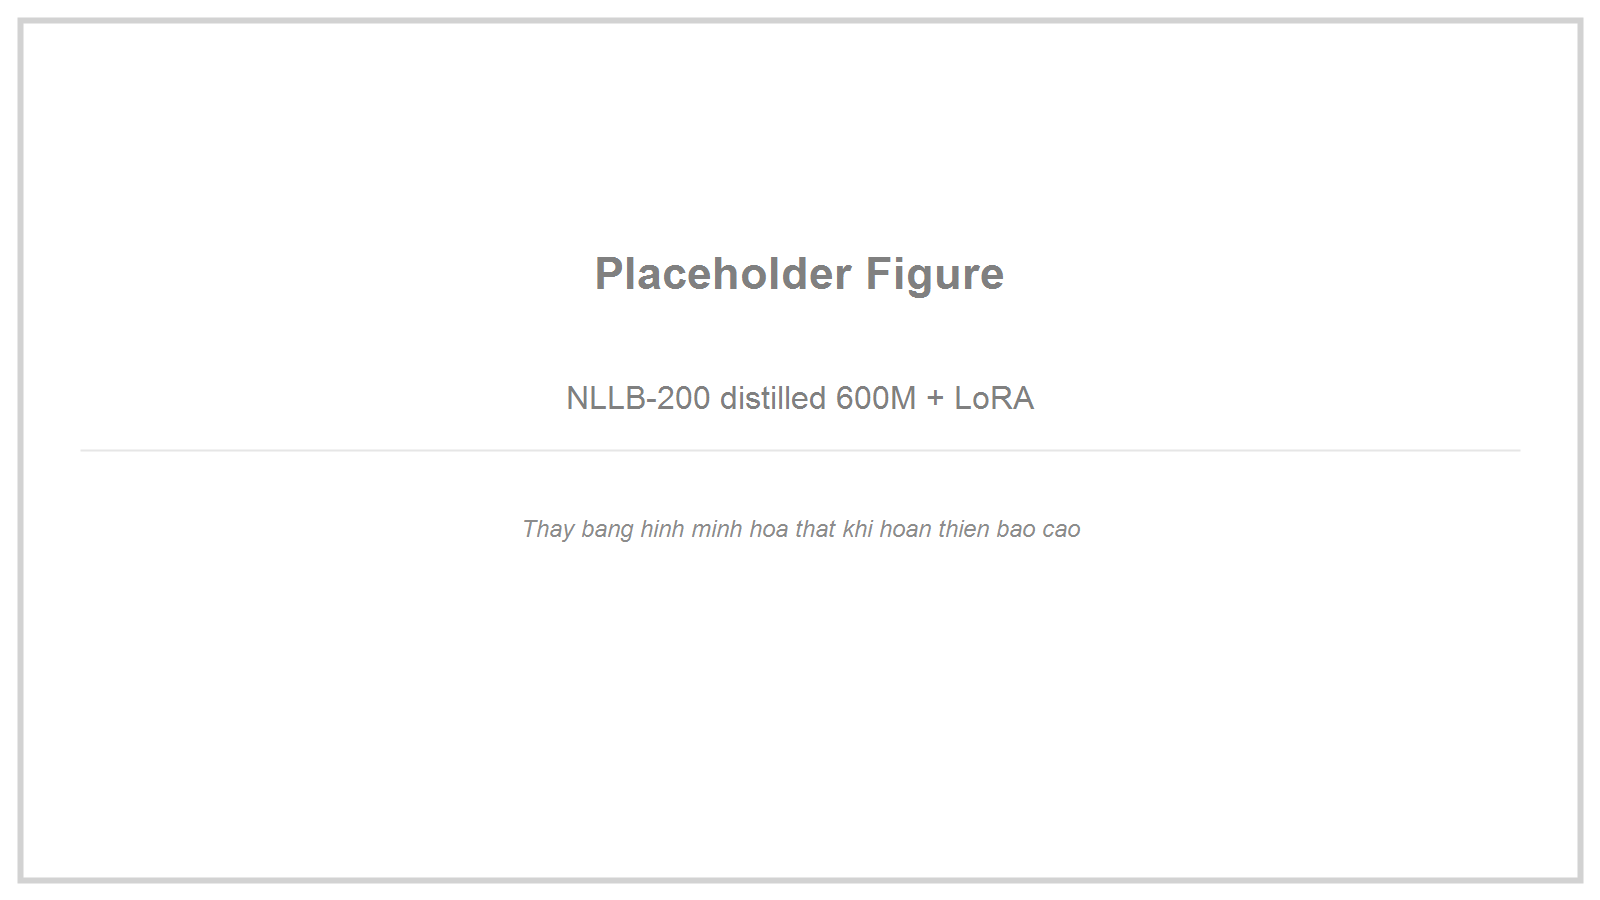
\includegraphics[width=0.84\textwidth]{figures/translation/nllb_lora_architecture.png}
\caption{Kiến trúc NLLB-200 kết hợp adapter LoRA trong mô-đun dịch Việt - Lào}
\label{fig:nllb-lora-architecture}
\end{figure}

\subsubsection{Tokenizer và cơ chế sinh câu đích}

Theo tài liệu chính thức của Hugging Face cho NLLB, tokenizer của họ mô hình này sử
dụng mã ngôn ngữ nguồn và ngôn ngữ đích như các \textit{special tokens}. Trong project,
quá trình suy luận được cấu hình như sau:
\begin{itemize}
    \item ngôn ngữ nguồn: \texttt{vie\_Latn};
    \item ngôn ngữ đích: \texttt{lao\_Laoo};
    \item ép token bắt đầu của câu đích bằng \texttt{forced\_bos\_token\_id};
    \item \texttt{max\_length = 128};
    \item \texttt{num\_beams = 5}.
\end{itemize}

Thiết kế này rất quan trọng. Nếu không đặt đúng mã ngôn ngữ hoặc không ép token bắt đầu
của tiếng đích, mô hình đa ngôn ngữ có thể sinh sai ngôn ngữ hoặc lẫn giữa nhiều miền dữ
liệu. Việc dùng \texttt{beam search} với 5 nhánh cũng cho phép mô hình ưu tiên những câu
dịch ổn định hơn so với giải mã tham lam đơn giản.

\subsubsection{Ưu điểm và những rủi ro cần lưu ý}

Điểm mạnh của hướng tiếp cận hiện tại là tận dụng được tri thức tiền huấn luyện đa ngôn
ngữ của NLLB, đồng thời dùng LoRA để hạ chi phí huấn luyện và lưu trữ. Điều này khiến
module dịch phù hợp với bối cảnh nghiên cứu ứng dụng, nơi khối lượng phần cứng thường
không đủ để full fine-tune các mô hình dịch cỡ lớn.

Tuy nhiên, mô-đun vẫn tồn tại một số rủi ro kỹ thuật:
\begin{itemize}
    \item chất lượng dịch phụ thuộc trực tiếp vào câu tiếng Việt đầu vào; nếu mô-đun ghép
    câu phía trước diễn đạt sai ý, mô-đun dịch sẽ khuếch đại lỗi đó;
    \item dữ liệu song ngữ hiện có khá dị miền, bao gồm hội thoại, câu kể, tên riêng và các
    câu mô tả dài, nên dễ phát sinh lỗi với thực thể riêng hoặc câu khẩu ngữ;
    \item một số mẫu dữ liệu quan sát được cho thấy còn hiện tượng nhiễu chính tả, viết hoa
    hoặc phiên âm tên riêng, có thể làm giảm tính ổn định của đầu ra.
\end{itemize}

Vì vậy, khi đánh giá mô-đun này, không nên chỉ nhìn vào một ví dụ dịch thành công, mà
cần đánh giá đồng thời bằng các metric dịch máy chuẩn và các ví dụ định tính nhiều miền.


\subsection{Cơ chế tích hợp giữa ba mô hình}

Việc tích hợp ba mô hình là nội dung quan trọng của đề tài vì chất lượng hệ thống không chỉ phụ thuộc vào từng mô-đun riêng lẻ mà còn phụ thuộc vào cách chúng truyền dữ liệu cho nhau. Trong project hiện tại, điểm ghép nối giữa các mô-đun được thiết kế theo kiểu dữ liệu trung gian đơn giản, dễ kiểm tra bằng mắt và dễ ghi log.

Tầng nhận diện trả về danh sách top-k nhãn ký hiệu kèm xác suất. Người dùng hoặc chương trình chọn nhãn phù hợp để đưa vào bộ đệm token. Vì mô hình nhận diện hiện tại là ASL-250, hệ thống cần bảng ánh xạ \texttt{ASL\_TO\_VI\_TOKEN} để chuyển nhãn tiếng Anh sang token tiếng Việt nội bộ. Ví dụ, nhãn \texttt{hello} được ánh xạ thành \texttt{xin\_chao}; nhãn \texttt{drink} có thể được ánh xạ thành token liên quan đến nhu cầu uống nước. Lớp ánh xạ này đóng vai trò adapter giữa miền thị giác ASL và miền NLP tiếng Việt.

Tầng khôi phục câu nhận bộ đệm token đã chuẩn hóa. Khi người dùng xác nhận, bộ đệm được nối thành chuỗi đầu vào cho \texttt{SentenceBuilder}. Kết quả sinh ra là một câu tiếng Việt đã viết hoa và có dấu câu. Câu này tiếp tục được chuyển sang mô-đun dịch Việt -- Lào. Nếu tắt tùy chọn dịch để chạy nhẹ hơn, pipeline vẫn hiển thị câu tiếng Việt và bỏ qua tầng NLLB.

Để giảm lỗi dây chuyền, hệ thống áp dụng một số chiến lược thực dụng: chỉ gom frame khi MediaPipe phát hiện tay, chỉ dự đoán khi đủ số frame tối thiểu, hiển thị top-k thay vì chỉ một nhãn, cho phép người dùng xác nhận token trước khi ghép câu và có chế độ chạy không tải mô hình dịch. Các cơ chế này không loại bỏ hoàn toàn sai số nhưng giúp quá trình demo ổn định hơn, đồng thời giúp xác định rõ lỗi xuất hiện ở tầng nhận diện, tầng ghép câu hay tầng dịch.


\subsection{Dữ liệu huấn luyện và tiền xử lý}

Ba mô-đun trong hệ thống sử dụng ba kiểu dữ liệu khác nhau: video RGB cho tầng nhận diện,
chuỗi gloss -- câu tiếng Việt cho tầng ghép câu, và cặp câu song ngữ Việt -- Lào cho tầng
dịch máy. Vì vậy, phần này không thể chỉ liệt kê tên dataset, mà cần mô tả rõ nguồn dữ liệu,
cách tổ chức mẫu, cách chia tập và các bước tiền xử lý cho từng mô-đun. Đây là cơ sở để người
đọc đánh giá tính hợp lệ của quá trình huấn luyện và thực nghiệm.

\subsubsection{Mô hình pre-trained cho mô-đun nhận diện ký hiệu}

Khác với hai mô-đun NLP phía sau (có quá trình huấn luyện rõ ràng trên dữ liệu riêng), mô-đun nhận
diện ký hiệu sử dụng một mô hình đã được huấn luyện sẵn (pre-trained). Cụ thể, hệ thống tích hợp
mô hình TFLite từ giải pháp đạt giải nhất cuộc thi Kaggle \textit{Google -- Isolated Sign Language
Recognition}.

Dữ liệu huấn luyện gốc của mô hình bao gồm:
\begin{itemize}
    \item 250 từ vựng ký hiệu ASL phổ biến;
    \item dữ liệu landmarks đã được trích xuất bằng MediaPipe Holistic (543 landmarks × 3 tọa độ);
    \item nhiều signer với điều kiện ghi hình đa dạng.
\end{itemize}

\begin{table}[H]
\centering
\caption{Thông tin mô hình pre-trained cho mô-đun nhận diện ký hiệu}
\label{tab:asl250-model-info}
\begin{tabularx}{\textwidth}{|X|c|}
\hline
\textbf{Thuộc tính} & \textbf{Giá trị} \\
\hline
Nguồn mô hình & Kaggle ASL Signs 1st Place Solution \\
\hline
Số lớp từ vựng & 250 \\
\hline
Định dạng mô hình & TensorFlow Lite (.tflite) \\
\hline
Kích thước file & $\sim$11 MB \\
\hline
Đầu vào mỗi frame & 543 landmarks × 3 tọa độ \\
\hline
Sliding window & 16--60 frames \\
\hline
\end{tabularx}
\end{table}

Vì nhóm không tự huấn luyện mô hình này, phần dữ liệu cho mô-đun nhận diện không có
train/validation/test split do nhóm thực hiện. Thay vào đó, các file cần thiết để chạy mô-đun
nhận diện bao gồm:
\begin{itemize}
    \item \texttt{model.tflite}: trọng số mô hình đã huấn luyện;
    \item \texttt{sign\_to\_prediction\_index\_map.json}: bảng ánh xạ giữa tên từ vựng ký hiệu
    và chỉ số đầu ra;
    \item \texttt{realtime\_asl\_250.py}: script suy luận thời gian thực.
\end{itemize}

Đây là một lựa chọn thiết kế có chủ đích: thay vì đầu tư toàn bộ thời gian vào việc tự huấn
luyện một mô hình nhận diện từ đầu (với rủi ro chất lượng không đảm bảo), nhóm lựa chọn tích
hợp một mô hình đã được kiểm chứng qua cuộc thi Kaggle, từ đó tập trung nguồn lực cho các tầng
NLP phía sau.

\subsubsection{Bộ dữ liệu cho mô-đun ghép câu tiếng Việt}

Theo tài liệu kỹ thuật trong \texttt{vsl.pdf}, mô-đun ghép câu được huấn luyện trên bộ dữ
liệu \textit{VSL Vietnamese NLP Dataset v4 Mega}. Bộ dữ liệu này bao gồm các cặp
\texttt{raw\_sentence} và \texttt{complete\_sentence}, trong đó:
\begin{itemize}
    \item \texttt{raw\_sentence} là chuỗi gloss hoặc chuỗi từ thô được chuẩn hóa từ ngôn
    ngữ ký hiệu;
    \item \texttt{complete\_sentence} là câu tiếng Việt hoàn chỉnh dùng làm nhãn đích.
\end{itemize}

\begin{figure}[H]
\centering
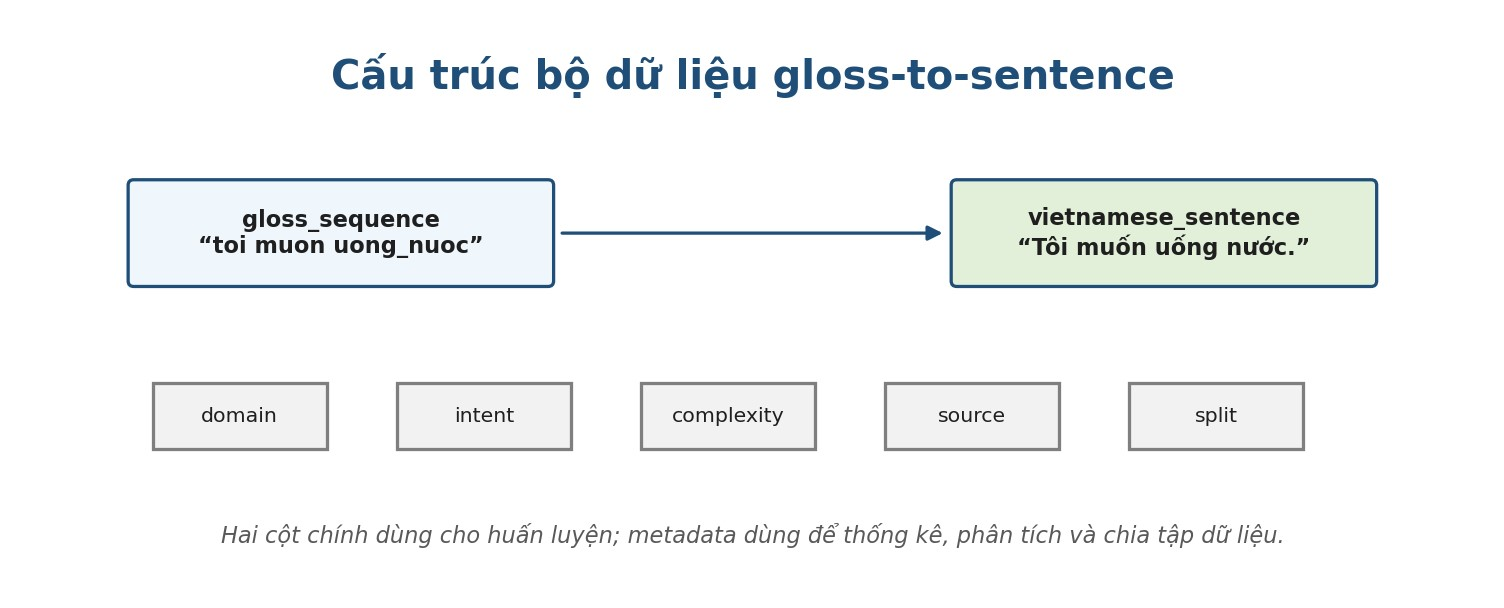
\includegraphics[width=0.82\textwidth]{figures/nlp/vsl_dataset_schema.jpg}
\caption{Cấu trúc một mẫu dữ liệu gloss-to-sentence}
\label{fig:vsl-dataset-schema}
\end{figure}

\begin{table}[H]
\centering
\caption{Thống kê bộ dữ liệu VSL Vietnamese NLP Dataset v4 Mega}
\begin{tabularx}{\textwidth}{|X|c|}
\hline
\textbf{Thuộc tính} & \textbf{Giá trị} \\
\hline
Tổng số mẫu câu & 32.755 \\
\hline
Số gloss token & 262 \\
\hline
Số nhóm ngữ cảnh & 32 \\
\hline
Train set & 26.204 \\
\hline
Validation set & 3.275 \\
\hline
Test set & 3.276 \\
\hline
\end{tabularx}
\end{table}

Bên cạnh bộ dữ liệu đầy đủ được mô tả trong tài liệu, snapshot mã nguồn hiện tại chỉ giữ
lại một tệp \texttt{data/sentence\_pairs.csv} gồm 50 dòng mẫu để phục vụ việc kiểm thử
tích hợp và minh họa cục bộ. Điều này cho thấy repository đang lưu phần tối thiểu cần cho
demo, còn bộ dữ liệu đầy đủ được quản lý bên ngoài ở giai đoạn huấn luyện chính thức.

\begin{figure}[H]
\centering
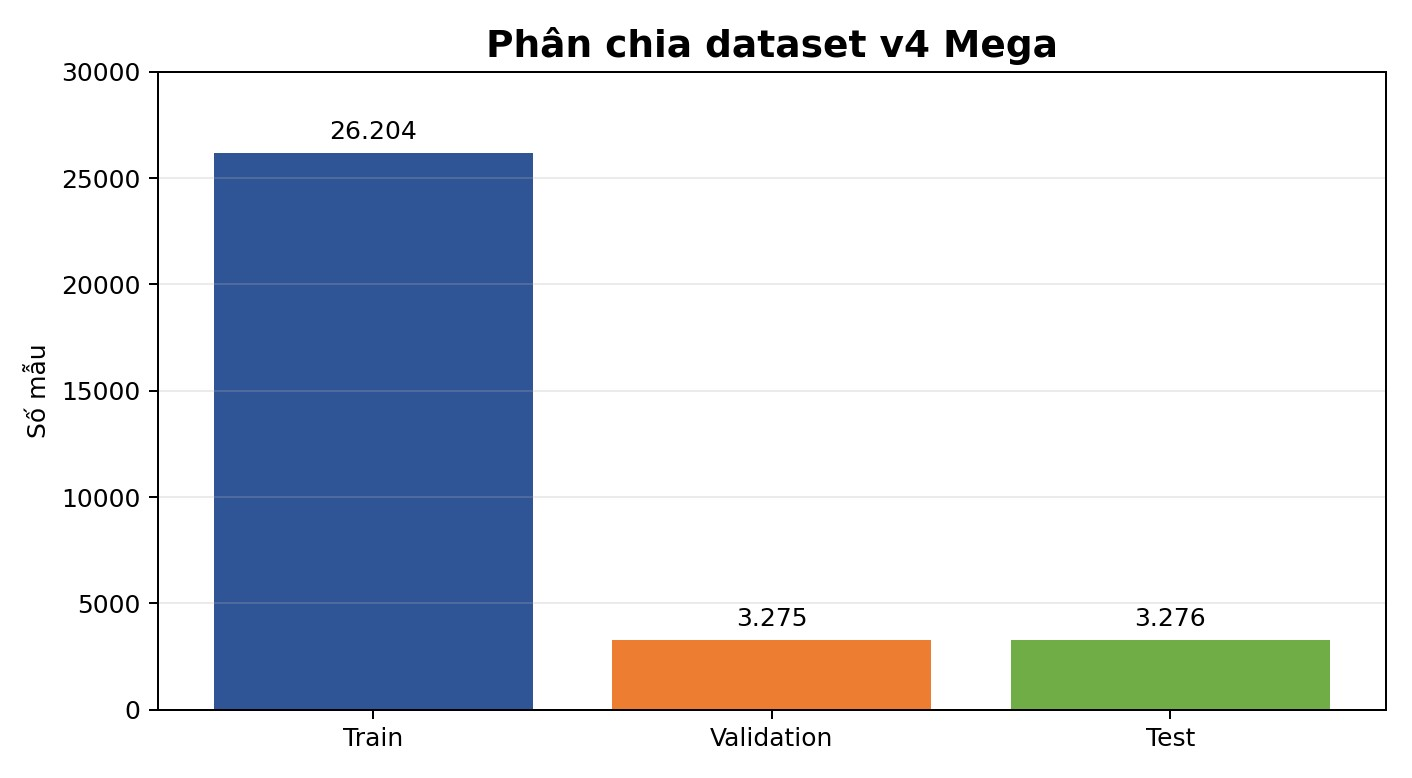
\includegraphics[width=0.82\textwidth]{figures/nlp/vsl_dataset_bar_split.jpg}
\caption{Số lượng mẫu trong các tập train, validation và test}
\label{fig:vsl-dataset-split}
\end{figure}

\begin{figure}[H]
\centering
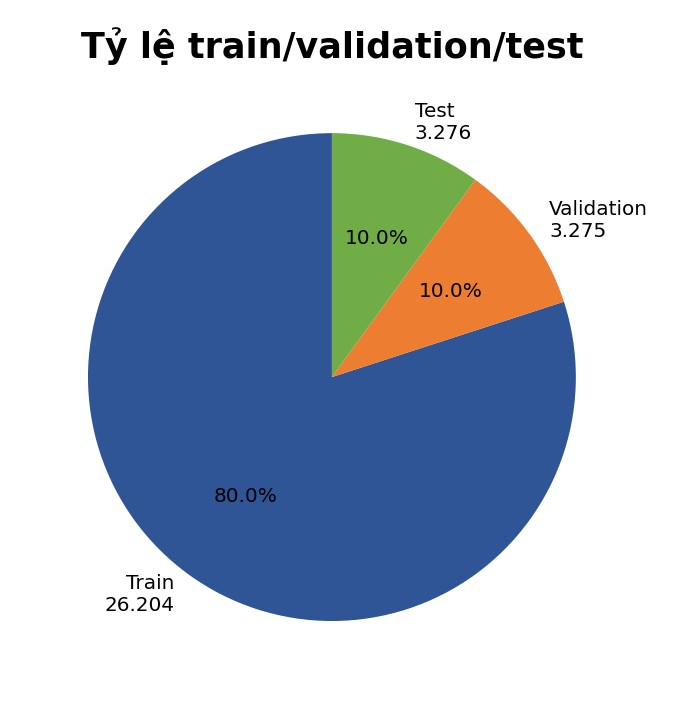
\includegraphics[width=0.55\textwidth]{figures/nlp/vsl_dataset_pie_split.jpg}
\caption{Tỷ lệ chia dữ liệu train, validation và test}
\label{fig:vsl-dataset-pie-split}
\end{figure}

\subsubsection{Tiền xử lý cho mô-đun ghép câu}

Tiền xử lý của mô-đun ghép câu được thực hiện theo đúng bản chất của dữ liệu gloss:
\begin{itemize}
    \item loại bỏ dòng rỗng hoặc giá trị \texttt{NaN};
    \item chuẩn hóa khoảng trắng đầu cuối và khoảng trắng thừa giữa các token;
    \item giữ lại các cụm từ ghép bằng dấu gạch dưới như \texttt{uong\_nuoc},
    \texttt{giup\_do}, \texttt{benh\_vien} để không làm mất đơn vị ý nghĩa;
    \item thêm tiền tố tác vụ \texttt{chuyen\_cau\_ky\_hieu:} vào đầu vào khi train và
    inference;
    \item token hóa bằng tokenizer của \texttt{vinai/bartpho-word-base};
    \item giới hạn độ dài đầu vào và đầu ra ở mức 64 token.
\end{itemize}

Việc giữ nguyên cấu trúc token dạng gloss là rất quan trọng. Nếu tách sai các cụm
\texttt{uong\_nuoc} hoặc \texttt{nha\_ve\_sinh}, mô hình sẽ phải học lại quan hệ ngữ nghĩa
phức tạp hơn và giảm tính ổn định trong quá trình sinh câu.

\subsubsection{Bộ dữ liệu cho mô-đun dịch Việt - Lào}

Tài liệu \texttt{vilo.pdf} mô tả dữ liệu dịch ở quy mô khoảng 100k câu song ngữ. Kiểm tra
thực tế trong repository hiện tại cho thấy thư mục
\codepath{dich-vi_lo/dataset/vi_lo_dataset_split} đã được chia sẵn thành ba tệp
\texttt{train.csv}, \texttt{valid.csv} và \texttt{test.csv}, với hai cột \texttt{vi} và
\texttt{lo}. Số lượng cụ thể như sau:

\begin{table}[H]
\centering
\caption{Thống kê dữ liệu song ngữ Việt - Lào trong repository}
\begin{tabularx}{\textwidth}{|X|c|}
\hline
\textbf{Thành phần} & \textbf{Số câu} \\
\hline
Train set & 90.000 \\
\hline
Validation set & 5.000 \\
\hline
Test set & 5.000 \\
\hline
Tổng số cặp câu & 100.000 \\
\hline
\end{tabularx}
\end{table}

Quan sát nhanh trên các mẫu dữ liệu cho thấy tập song ngữ này khá đa miền: có câu hội
thoại đời thường, câu kể, câu mô tả, tên riêng và câu văn dài. Đây là ưu điểm về độ phủ,
nhưng đồng thời cũng tạo ra thách thức vì dữ liệu có thể chứa nhiễu ở tên riêng, viết hoa,
phiên âm hoặc các cấu trúc câu không đồng đều.

\begin{figure}[H]
\centering
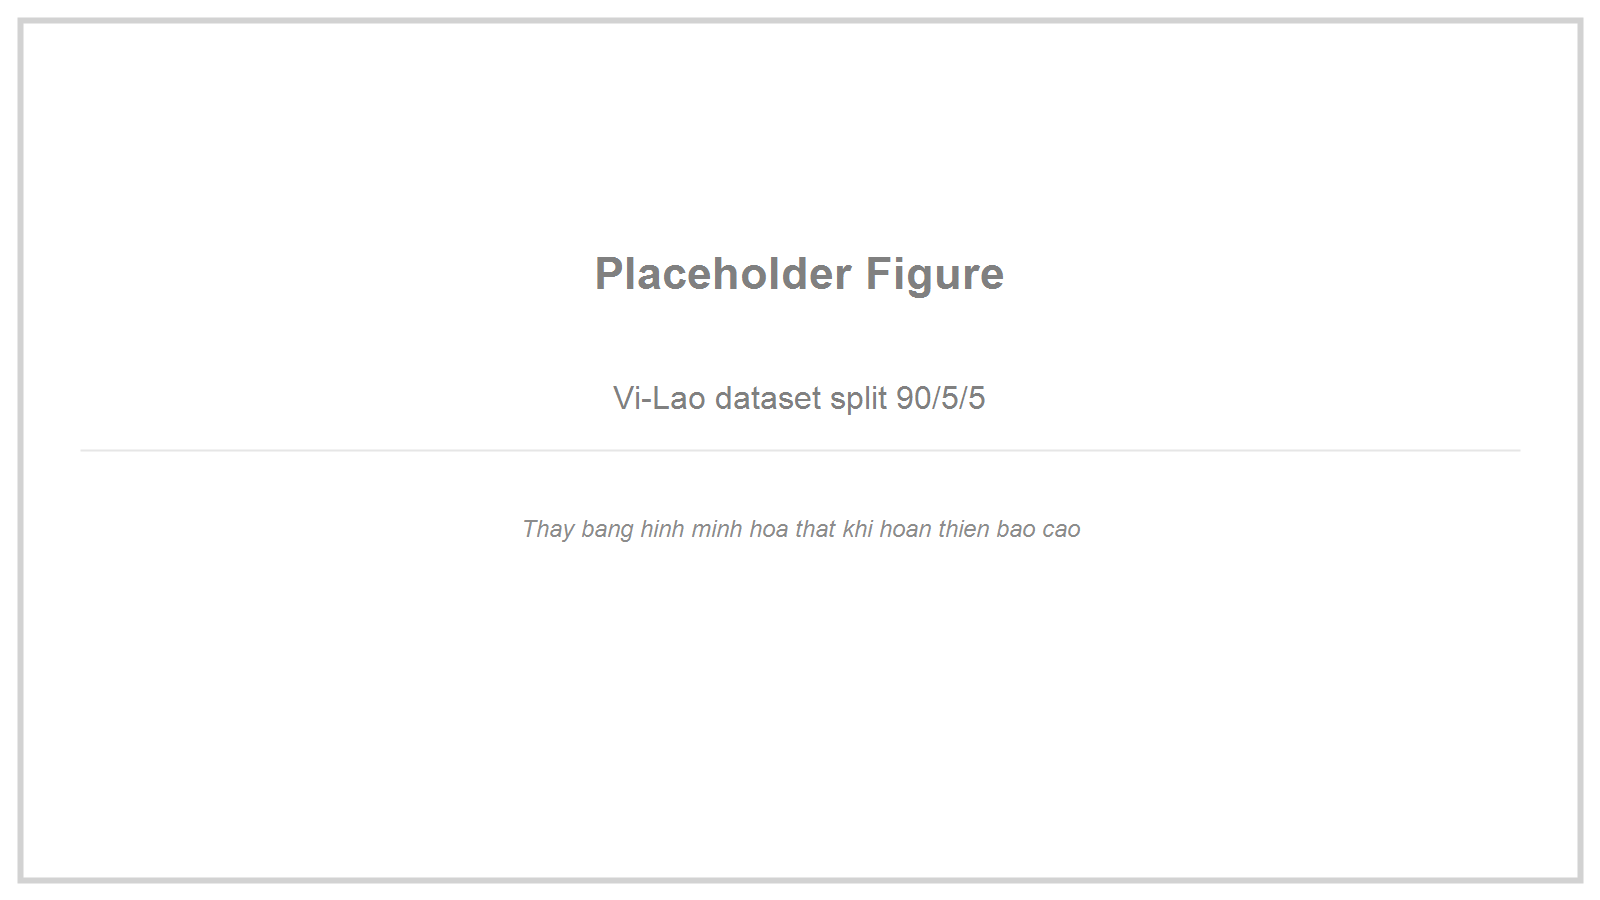
\includegraphics[width=0.82\textwidth]{figures/translation/translation_dataset_split.png}
\caption{Tỉ lệ chia bộ dữ liệu song ngữ Việt -- Lào}
\label{fig:vi-lao-dataset-split}
\end{figure}

\subsubsection{Tiền xử lý cho mô-đun dịch Việt - Lào}

So với mô-đun ghép câu, tiền xử lý của mô-đun dịch tập trung nhiều hơn vào tokenizer đa
ngôn ngữ của NLLB. Trong bản hiện thực hiện tại, các bước chính có thể tóm tắt như sau:
\begin{itemize}
    \item dữ liệu đã được tách sẵn theo câu trong các tệp CSV;
    \item cột nguồn là tiếng Việt, cột đích là tiếng Lào;
    \item tokenizer của NLLB gắn mã ngôn ngữ nguồn \texttt{vie\_Latn} và ngôn ngữ đích
    \texttt{lao\_Laoo};
    \item mô hình sử dụng token hóa kiểu subword của NLLB để giảm vấn đề từ ngoài từ
    điển;
    \item khi suy luận, mô hình được ép bắt đầu bằng token ngôn ngữ tiếng Lào để tránh
    sinh nhầm ngôn ngữ đích.
\end{itemize}

Trong thực nghiệm sau này, nếu cần nâng chất lượng mô hình, hai hướng tiền xử lý nên ưu
tiên là: làm sạch tên riêng và thống nhất quy tắc viết hoa, dấu câu trên cặp dữ liệu song
ngữ. Đây là hai nguồn nhiễu dễ gặp nhất trong tập dữ liệu quan sát được tại thời điểm viết
báo cáo.



\clearpage


\section{XÂY DỰNG PHẦN MỀM VÀ TÍCH HỢP HỆ THỐNG}

\subsection{Yêu cầu chức năng và phi chức năng}

Trước khi đi vào cài đặt, hệ thống cần được đặc tả bằng các yêu cầu chức năng và phi chức năng. Việc đặc tả rõ ràng giúp liên hệ trực tiếp giữa mục tiêu nghiên cứu ở Chương 1 và phần hiện thực phần mềm ở Chương 3.

\subsubsection{Yêu cầu chức năng}
\begin{itemize}
    \item Nhận video từ webcam theo thời gian thực.
    \item Nhận diện ký hiệu và hiển thị kết quả dự đoán.
    \item Lưu buffer từ vựng và ghép thành câu tiếng Việt.
    \item Dịch câu tiếng Việt sang tiếng Lào.
    \item Cho phép xóa buffer, xác nhận câu và thoát chương trình.
\end{itemize}

\subsubsection{Yêu cầu phi chức năng}
\begin{itemize}
    \item Thời gian phản hồi đủ nhanh để demo trực tiếp.
    \item Hệ thống dễ mở rộng thêm lớp ký hiệu và thêm ngôn ngữ đích.
    \item Cấu trúc code tách mô-đun để dễ bảo trì.
    \item Có khả năng chạy ở chế độ giảm tải khi không muốn nạp mô hình dịch lớn.
    \item Có cơ chế fallback để tầng NLP vẫn sinh được câu tối thiểu khi mô hình sinh chưa sẵn sàng.
\end{itemize}

Các yêu cầu này dẫn đến lựa chọn thiết kế mô-đun hóa: nhận diện, ghép câu và dịch máy được giữ thành các khối độc lập, có thể kiểm thử riêng trước khi tích hợp. Đây cũng là lý do project có cả script kiểm thử dạng dòng lệnh và script realtime dùng webcam.


\subsection{Phân tích use case}

Phần use case giúp liên kết bài toán kỹ thuật với hành vi sử dụng thực tế của người dùng. Đối với đề tài này, actor chính là người vận hành hệ thống hoặc người dùng cần thực hiện nhận diện và dịch ngôn ngữ ký hiệu.

\begin{enumerate}
    \item \textbf{Khởi động hệ thống và webcam}: người vận hành chạy chương trình realtime, hệ thống nạp MediaPipe, mô hình TFLite và các cấu hình cần thiết.
    \item \textbf{Thực hiện ký hiệu}: người dùng đưa tay vào khung hình và thực hiện ký hiệu. Hệ thống trích xuất landmarks, duy trì bộ đệm frame và hiển thị top-k nhãn dự đoán.
    \item \textbf{Xác nhận token}: khi nhãn hiện tại phù hợp, người vận hành thêm nhãn đó vào buffer token. Bước này giúp giảm tác động của các dự đoán nhiễu.
    \item \textbf{Sinh câu và dịch}: khi buffer đã đủ nội dung, người vận hành yêu cầu hệ thống ghép thành câu tiếng Việt và dịch sang tiếng Lào nếu mô hình dịch đang bật.
    \item \textbf{Xóa buffer hoặc bắt đầu lại}: nếu nhận diện sai hoặc người dùng muốn nhập câu mới, hệ thống cho phép xóa buffer token và reset bộ đệm frame.
    \item \textbf{Kết thúc phiên làm việc}: người vận hành thoát chương trình, giải phóng camera và đóng cửa sổ hiển thị.
\end{enumerate}

Luồng use case trên phản ánh đúng hiện trạng triển khai: hệ thống chưa tự động quyết định toàn bộ câu dài liên tục, mà có bước xác nhận token để tăng độ ổn định trong demo. Đây là lựa chọn phù hợp với giai đoạn nguyên mẫu vì người dùng vẫn kiểm soát được đầu vào của tầng NLP và tầng dịch.


\subsection{Xây dựng mô-đun nhận diện ký hiệu}

Nếu Chương 2 tập trung vào việc lý giải vì sao chọn MediaPipe Holistic và mô hình TFLite pre-trained
(Kaggle ASL Signs), thì phần này mô tả cách mô-đun đã được hiện thực thành mã nguồn cụ thể. Ở
snapshot hiện tại, module nhận diện được tổ chức gọn trong thư mục \texttt{external/asl_baseline/},
bao gồm file mô hình, bảng ánh xạ nhãn và script suy luận thời gian thực.

\subsubsection{Cấu trúc mã nguồn của mô-đun}

\begin{table}[H]
\centering
\caption{Các file chính của mô-đun nhận diện}
\label{tab:recognition-files}
\begin{tabularx}{\textwidth}{|>{\raggedright\arraybackslash}p{5.4cm}|X|}
\hline
\textbf{File} & \textbf{Vai trò} \\
\hline
\codepath{external/asl_baseline/realtime_asl_250.py} & Chương trình webcam thời gian thực: khởi tạo TFLite Interpreter, đọc camera, duy trì sliding window landmarks, suy luận mô hình và hiển thị top-k dự đoán. \\
\hline
\codepath{external/asl_baseline/model.tflite} & Trọng số mô hình đã huấn luyện sẵn, giải pháp đạt giải nhất cuộc thi Kaggle ASL Signs. Kích thước $\sim$11 MB. \\
\hline
\codepath{external/asl_baseline/sign_to_prediction_index_map.json} & Bảng ánh xạ 250 tên từ vựng ký hiệu sang chỉ số đầu ra tương ứng của mô hình. \\
\hline
\codepath{external/asl_baseline/MODEL_README.md} & Tài liệu ghi chú nguồn gốc mô hình và giấy phép MIT. \\
\hline
\end{tabularx}
\end{table}

Cấu trúc này rất gọn so với các mô-đun NLP: toàn bộ logic nhận diện được đóng gói trong một file
Python duy nhất, kèm theo mô hình TFLite và bảng nhãn. Việc sử dụng mô hình pre-trained giúp giảm
đáng kể số lượng file cần quản lý, không cần notebook huấn luyện hay checkpoint riêng.

\subsubsection{Hiện thực trích xuất landmarks bằng MediaPipe}

Lớp \texttt{ASL250Recognizer} trong \texttt{realtime\_asl\_250.py} khởi tạo MediaPipe Holistic với
cấu hình:
\begin{itemize}
    \item \texttt{model\_complexity=1};
    \item \texttt{refine\_face\_landmarks=False};
    \item \texttt{min\_detection\_confidence=0.5};
    \item \texttt{min\_tracking\_confidence=0.5}.
\end{itemize}

Hàm \texttt{\_extract\_frame\_landmarks(results)} là điểm vào quan trọng nhất của tầng thị giác.
Luồng xử lý gồm các bước:
\begin{enumerate}
    \item lấy landmarks khuôn mặt (468 điểm), tay trái (21 điểm), pose (33 điểm) và tay phải
    (21 điểm);
    \item mỗi nhóm landmarks được trải phẳng thành ma trận \texttt{(N, 3)} với tọa độ
    \texttt{(x, y, z)};
    \item nếu thiếu bất kỳ nhóm landmark nào (ví dụ tay không xuất hiện), thay bằng ma trận
    \texttt{NaN} cùng kích thước;
    \item nối bốn nhóm theo thứ tự \texttt{face, left\_hand, pose, right\_hand} thành ma trận
    cuối cùng kích thước \texttt{(543, 3)}.
\end{enumerate}

Thiết kế ``điền NaN khi thiếu landmark'' là một chi tiết kỹ thuật quan trọng, khác biệt so với
phương pháp điền zero thông thường. Giá trị \texttt{NaN} cho phép mô hình TFLite phân biệt rõ
giữa ``không có dữ liệu'' và ``tọa độ bằng 0'', từ đó tránh tạo nhiễu đầu vào không cần thiết.

Thứ tự nối landmarks (face → left\_hand → pose → right\_hand) tuân theo quy ước của cuộc thi
Kaggle ASL Signs và phải được giữ nguyên để đảm bảo tương thích với mô hình pre-trained.

\subsubsection{Hiện thực nạp và suy luận mô hình TFLite}

Trong phương thức khởi tạo, mô hình TFLite được nạp bằng TensorFlow Lite Interpreter.
Quá trình khởi tạo gồm:
\begin{itemize}
    \item nạp file \texttt{model.tflite};
    \item lưu lại chỉ số tensor đầu vào (\texttt{input\_index}) và đầu ra
    (\texttt{output\_index});
    \item nạp bảng ánh xạ nhãn từ \texttt{sign\_to\_prediction\_index\_map.json};
    \item tạo ánh xạ ngược \texttt{id\_to\_sign} để chuyển từ chỉ số sang tên từ vựng.
\end{itemize}

Phương thức \texttt{predict()} thực hiện suy luận theo các bước:
\begin{enumerate}
    \item kiểm tra bộ đệm đã đủ tối thiểu 16 frame chưa;
    \item gom toàn bộ frames trong bộ đệm thành tensor đầu vào;
    \item gọi \texttt{resize\_tensor\_input()} để điều chỉnh kích thước đầu vào theo số frame
    thực tế;
    \item gọi \texttt{allocate\_tensors()}, \texttt{set\_tensor()};
    \item gọi \texttt{invoke()} để chạy suy luận;
    \item lấy kết quả từ \texttt{get\_tensor()};
    \item áp dụng softmax nếu đầu ra chưa ở dạng xác suất;
    \item trả về top-k nhãn có xác suất cao nhất.
\end{enumerate}

Một chi tiết đáng chú ý là hàm \texttt{\_softmax\_if\_needed()}: hàm này kiểm tra xem đầu ra
của mô hình đã ở dạng xác suất (tổng $\approx$ 1, tất cả $\geq$ 0) hay chưa. Nếu chưa, nó tự
động áp dụng softmax. Thiết kế này giúp code hoạt động ổn định bất kể mô hình TFLite trả về
logits hay xác suất.

\subsubsection{Hiện thực suy luận thời gian thực}

Trong phương thức \texttt{run()}, luồng chạy chính của mô-đun nhận diện có thể tóm tắt như sau:
\begin{enumerate}
    \item mở webcam với độ phân giải 960x540;
    \item với mỗi frame: lật ảnh như gương, chuyển sang RGB và xử lý bằng MediaPipe Holistic;
    \item chỉ gom landmarks vào bộ đệm khi phát hiện có bàn tay (trái hoặc phải);
    \item mỗi 8 frame (\texttt{predict\_every=8}), gọi \texttt{predict()} nếu bộ đệm đủ
    16 frame;
    \item hiển thị top-3 dự đoán trên giao diện video;
    \item vẽ skeleton pose và bàn tay lên khung hình bằng MediaPipe drawing utilities.
\end{enumerate}

Từ góc nhìn trải nghiệm người dùng, ba cơ chế nhỏ nhưng hiệu quả là:
\begin{itemize}
    \item \textbf{chỉ gom khi có tay}: lọc các frame không có ý nghĩa ký hiệu;
    \item \textbf{predict\_every = 8}: giảm tải tính toán, không cần suy luận mỗi frame;
    \item \textbf{min\_frames = 16}: đảm bảo mô hình có đủ ngữ cảnh thời gian trước khi
    dự đoán.
\end{itemize}

Hai phím điều khiển chính:
\begin{itemize}
    \item \texttt{Space}: reset bộ đệm và kết quả dự đoán;
    \item \texttt{q}: thoát chương trình.
\end{itemize}

\begin{figure}[H]
\centering
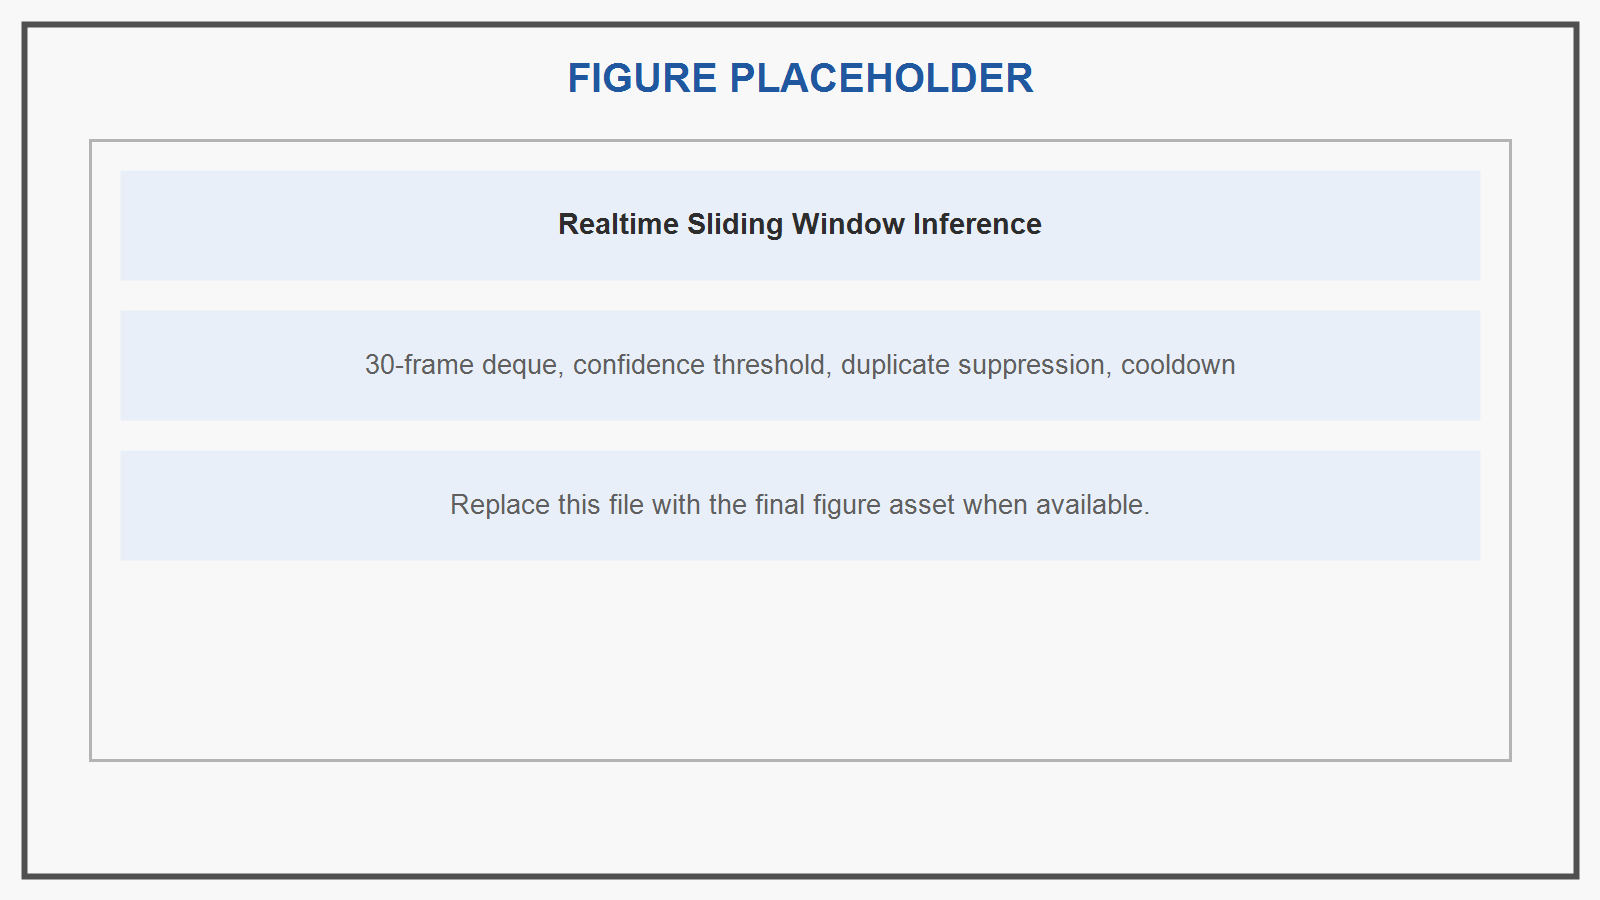
\includegraphics[width=0.84\textwidth]{figures/recognition/realtime_sliding_window.png}
\caption{Sơ đồ sliding window 16--60 frame và logic ``chỉ gom khi có tay'' trong suy luận realtime}
\label{fig:realtime-sliding-window}
\end{figure}

\subsubsection{Nhận xét dưới góc nhìn kỹ thuật phần mềm}

Mô-đun nhận diện hiện tại có nhiều điểm làm tốt ở khía cạnh phần mềm:
\begin{itemize}
    \item toàn bộ logic được đóng gói trong một lớp \texttt{ASL250Recognizer} duy nhất, dễ
    tích hợp và tái sử dụng;
    \item giao diện giữa mô-đun nhận diện và mô-đun NLP chỉ là nhãn gloss, nên dễ tích hợp;
    \item mô hình TFLite chạy trên CPU, không yêu cầu GPU, phù hợp với phần cứng phổ thông;
    \item code hỗ trợ nhiều camera backend (\texttt{CAP\_DSHOW} trên Windows,
    \texttt{CAP\_ANY} trên các hệ điều hành khác);
    \item có argparse để cấu hình camera, max-frames, min-frames từ dòng lệnh.
\end{itemize}

Bên cạnh đó cũng có vài giới hạn cần ghi nhận trung thực trong báo cáo:
\begin{itemize}
    \item phần tích hợp với mô-đun NLP phía sau (ghép câu tiếng Việt, dịch Việt - Lào) chưa
    được nối trực tiếp trong script hiện tại; cần thêm bước ánh xạ gloss tiếng Anh sang token
    tiếng Việt;
    \item vì là mô hình pre-trained, nhóm không thể can thiệp vào kiến trúc bên trong hoặc tinh
    chỉnh thêm cho VSL;
    \item cấu hình hiện tại nhắm tới demo một người, một webcam, chưa phải bài toán nhiều người
    đồng thời hoặc bối cảnh nền phức tạp.
\end{itemize}

Nhìn chung, ở mức đồ án môn học, mô-đun này đã đạt một ngưỡng hiện thực hóa đầy đủ: có mô hình
pre-trained chất lượng cao, có script suy luận realtime và có cổng nối lên tầng NLP thông qua đầu
ra gloss.


\subsection{Xây dựng mô-đun ghép từ thành câu tiếng Việt}

Nếu Chương 2 tập trung vào việc giải thích vì sao chọn kiến trúc lai
Rule-based, BARTpho và fallback, thì phần này trình bày cách mô-đun được hiện thực
hóa trong mã nguồn và cách nó tham gia vào pipeline phần mềm tổng thể. Điểm quan trọng
nhất là project không coi bài toán ghép câu như một khối ``black-box'', mà tách rõ thành
nhiều lớp xử lý nhỏ để dễ kiểm thử và dễ tích hợp.

\subsubsection{Các thành phần chính trong mã nguồn}

Mô-đun ghép câu được tổ chức xoay quanh bốn thành phần:
\begin{itemize}
    \item \textbf{\texttt{SentenceBuilder}}: điều phối toàn bộ quá trình nhận chuỗi gloss,
    chọn đường xử lý phù hợp và trả về câu hoàn chỉnh.
    \item \textbf{\texttt{sentence\_rules.json}}: tập luật cứng cho các mẫu câu thường gặp,
    có tính xác định cao.
    \item \textbf{\texttt{BartphoSentencePredictor}}: nạp tokenizer, mô hình đã fine-tune
    và thực hiện suy luận sinh câu.
    \item \textbf{\texttt{fallback\_corrector}}: ánh xạ các token cơ bản sang tiếng Việt và
    hoàn thiện định dạng câu khi mô hình chưa sẵn sàng.
\end{itemize}

\begin{table}[H]
\centering
\caption{Vai trò của các file quan trọng trong mô-đun ghép câu}
\begin{tabularx}{\textwidth}{|>{\raggedright\arraybackslash}p{5cm}|X|}
\hline
\textbf{File} & \textbf{Chức năng} \\
\hline
\codepath{src/nlp/sentence_builder.py} & Điều phối thứ tự ưu tiên rule, sau đó BARTpho, rồi fallback. \\
\hline
\codepath{src/nlp/bartpho_predictor.py} & Nạp mô hình đã fine-tune và sinh câu tiếng Việt bằng \texttt{beam search}. \\
\hline
\codepath{src/nlp/fallback_corrector.py} & Chuẩn hóa token, ánh xạ từ thô và thêm viết hoa, dấu câu. \\
\hline
\codepath{configs/sentence_rules.json} & Lưu các mẫu câu tần suất cao để phản hồi nhanh và ổn định. \\
\hline
\codepath{configs/nlp_config.json} & Lưu cấu hình huấn luyện và suy luận của BARTpho. \\
\hline
\end{tabularx}
\end{table}

\begin{figure}[H]
\centering
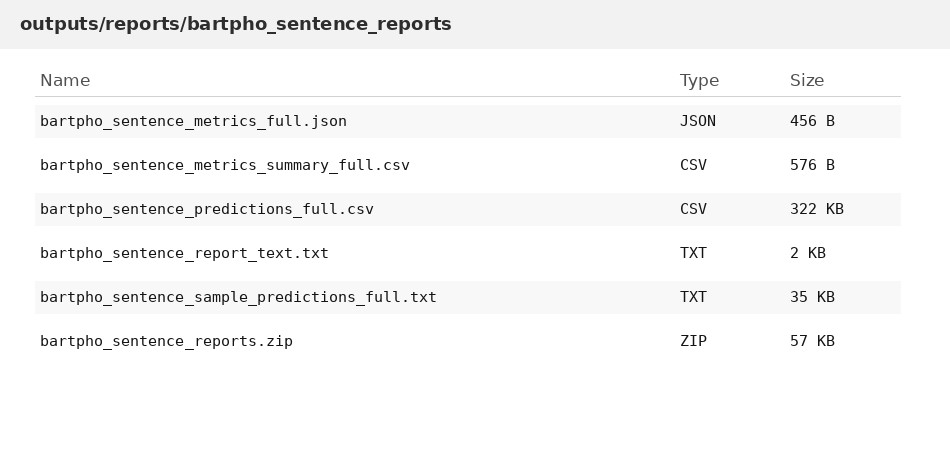
\includegraphics[width=0.78\textwidth]{figures/nlp/vsl_report_files.jpg}
\caption{Các file báo cáo được sinh sau khi đánh giá mô hình}
\label{fig:vsl-report-files}
\end{figure}

\subsubsection{Luồng xử lý chính}

Trong lớp \texttt{SentenceBuilder}, đầu vào trước hết được chuẩn hóa bằng cách loại bỏ
khoảng trắng thừa. Sau đó hệ thống xử lý theo thứ tự ưu tiên:
\begin{enumerate}
    \item nếu chuỗi đầu vào rỗng, trả về chuỗi rỗng;
    \item nếu chuỗi đầu vào khớp đúng một rule trong \texttt{sentence\_rules.json}, trả về
    câu rule tương ứng;
    \item nếu BARTpho đã được nạp thành công, gọi hàm \texttt{predict()} để sinh câu;
    \item nếu mô hình chưa có hoặc nạp lỗi, gọi \texttt{normalize\_raw\_text()} và
    \texttt{to\_sentence()} để rơi về chế độ dự phòng.
\end{enumerate}

Thứ tự này có ý nghĩa thực tiễn rất rõ:
\begin{itemize}
    \item rule-based đảm bảo các câu giao tiếp quan trọng như xin chào, xin lỗi, yêu cầu
    hỗ trợ luôn cho kết quả ổn định;
    \item BARTpho đảm nhiệm những trường hợp chuỗi gloss dài hơn hoặc linh hoạt hơn;
    \item fallback giúp hệ thống không bị ``gãy'' khi thiếu mô hình huấn luyện.
\end{itemize}

\begin{figure}[H]
\centering
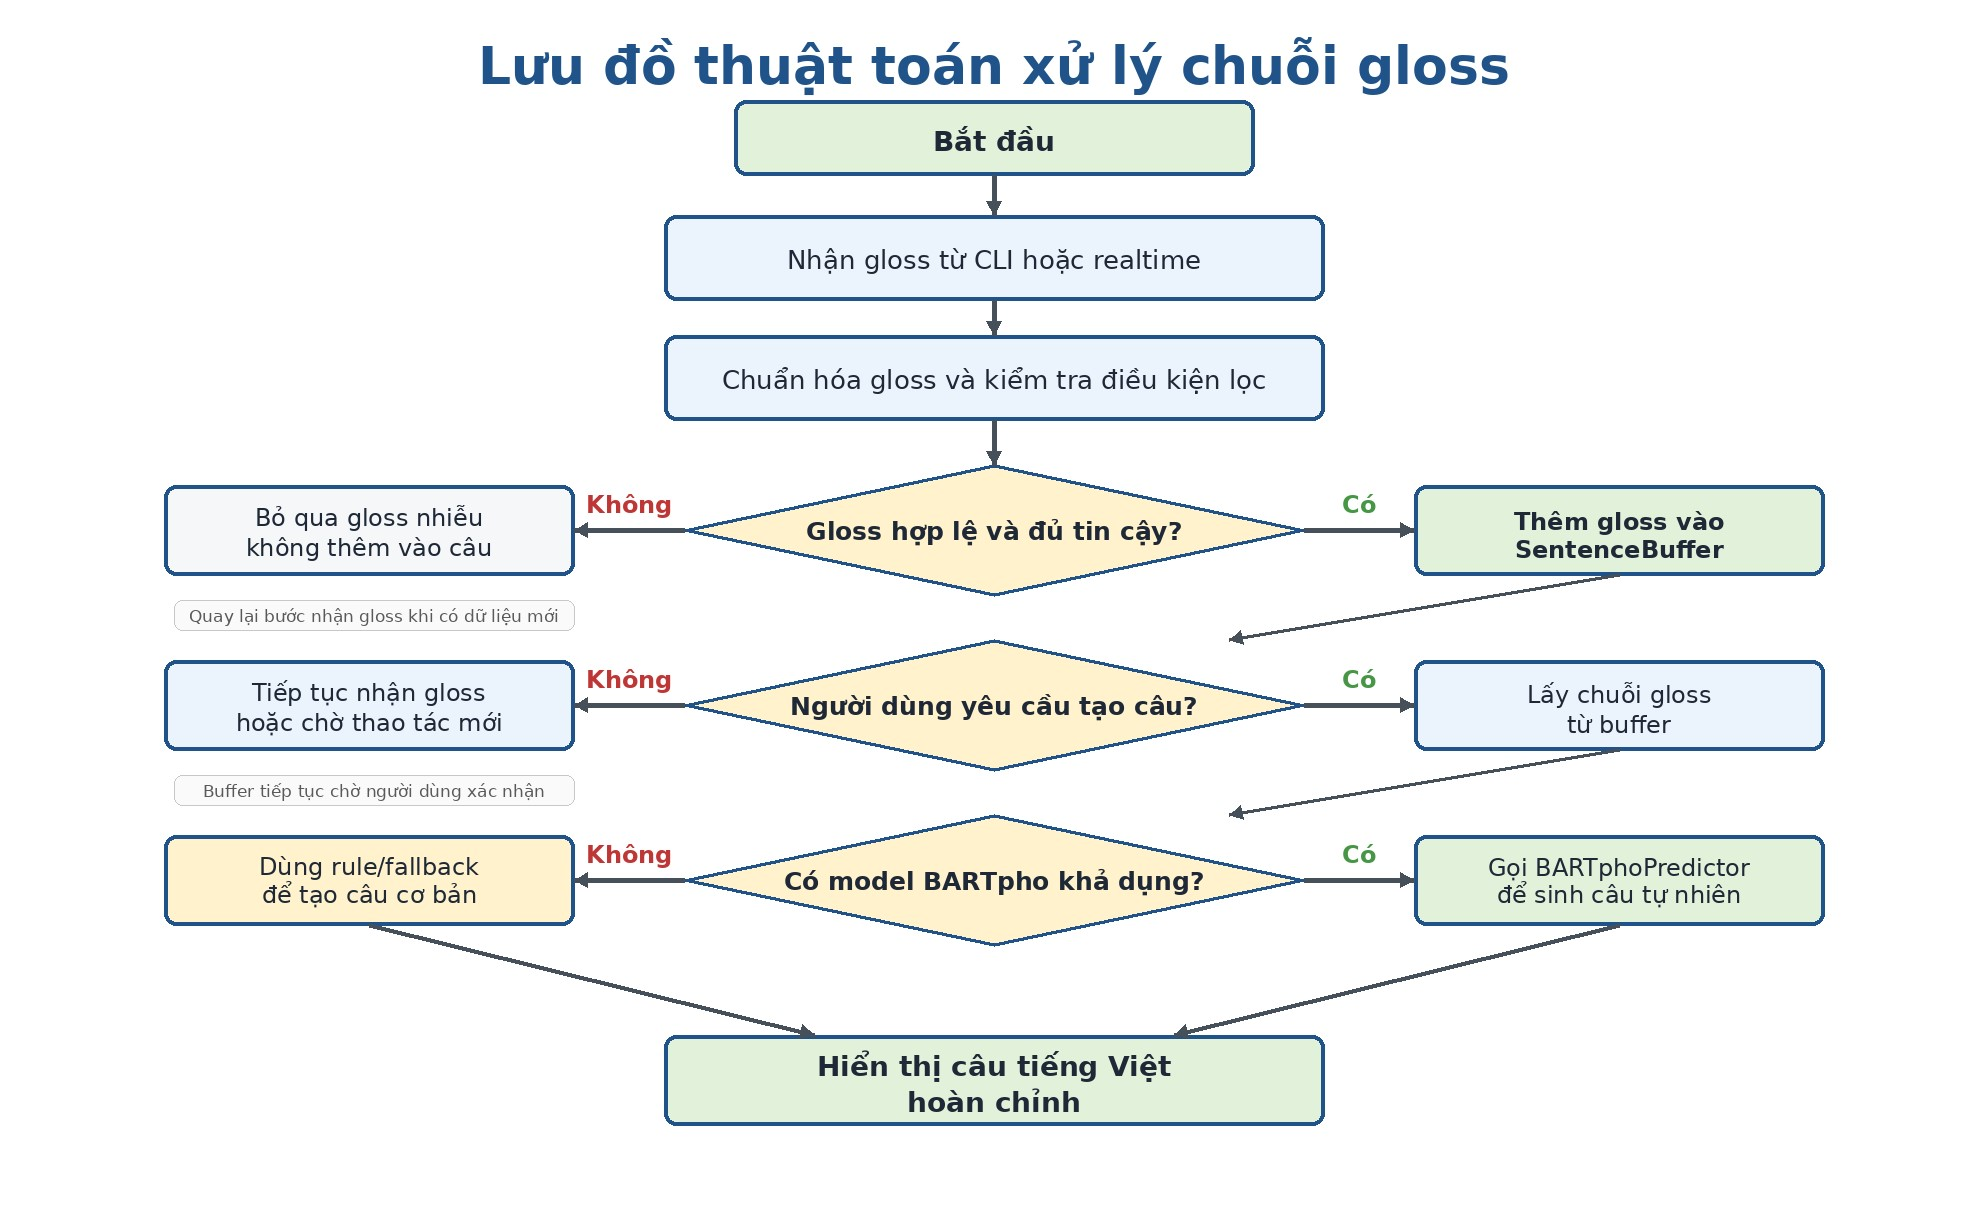
\includegraphics[width=0.94\textwidth]{figures/nlp/vsl_gloss_processing_flowchart.jpg}
\caption{Lưu đồ xử lý chuỗi gloss trong mô-đun ghép câu}
\label{fig:sentence-builder-runtime}
\end{figure}

\subsubsection{Hiện thực tầng rule-based và fallback}

Tầng rule-based được hiện thực bằng một tệp JSON đơn giản, trong đó mỗi khóa là một
chuỗi gloss chuẩn hóa, còn giá trị là câu tiếng Việt đích. Cách làm này tuy đơn giản nhưng
rất hiệu quả với các mẫu câu ngắn và các cụm ý nghĩa gần như cố định trong miền giao
tiếp hỗ trợ, ví dụ:
\begin{itemize}
    \item \texttt{xin\_chao} cho ra câu \textit{Xin chào.}
    \item \texttt{toi can giup\_do} cho ra câu \textit{Tôi cần giúp đỡ.}
    \item \texttt{toi muon uong\_nuoc} cho ra câu \textit{Tôi muốn uống nước.}
\end{itemize}

Trong trường hợp không có mô hình sinh câu, file \texttt{fallback\_corrector.py} dùng một
bảng ánh xạ token như \texttt{toi} thành \textit{tôi}, \texttt{uong\_nuoc} thành
\textit{uống nước}, \texttt{bac\_si} thành \textit{bác sĩ}. Sau khi ghép các từ lại, hệ thống tự viết hoa ký
tự đầu và thêm dấu chấm nếu cuối câu chưa có dấu kết thúc. Nhờ đó, ngay cả khi chỉ chạy
ở chế độ dự phòng, đầu ra vẫn đọc được và đủ dùng trong các demo tối thiểu.

\begin{figure}[H]
\centering
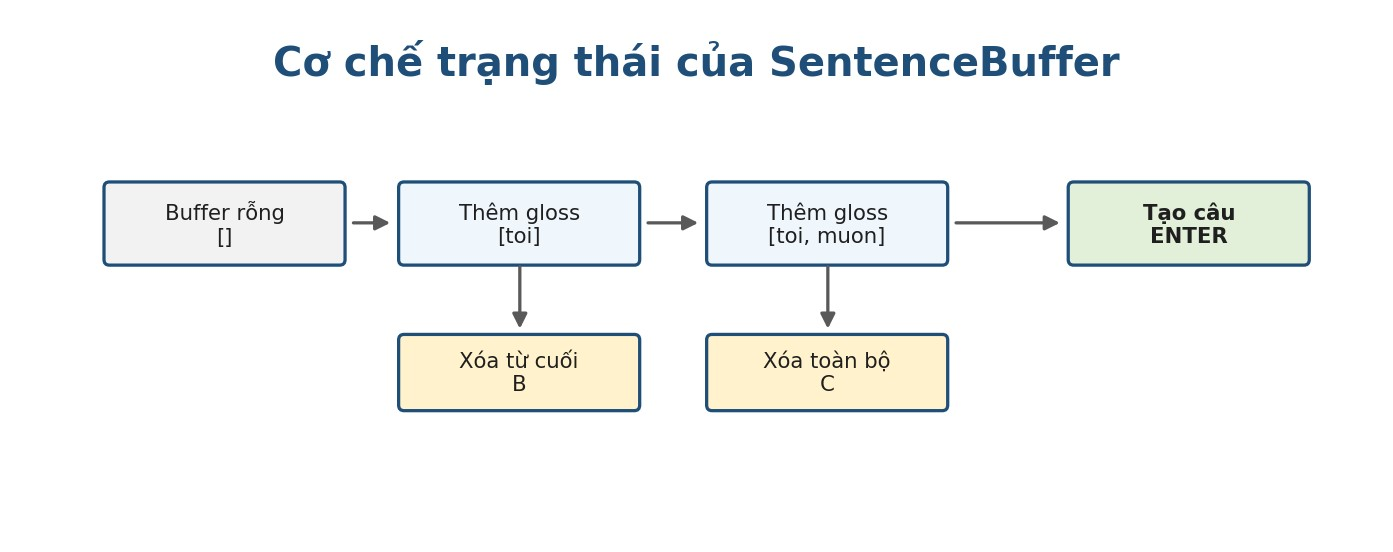
\includegraphics[width=0.82\textwidth]{figures/nlp/vsl_sentence_buffer_state_machine.jpg}
\caption{Cơ chế trạng thái của \texttt{SentenceBuffer} khi thêm, xoá và tạo câu}
\label{fig:vsl-sentence-buffer-state-machine}
\end{figure}

\subsubsection{Hiện thực suy luận bằng BARTpho}

Lớp \texttt{BartphoSentencePredictor} chịu trách nhiệm nạp mô hình từ thư mục
\texttt{models/bartpho\_sentence}. Quá trình suy luận gồm các bước:
\begin{itemize}
    \item chuẩn hóa lại chuỗi đầu vào;
    \item thêm tiền tố nhiệm vụ \texttt{chuyen\_cau\_ky\_hieu:};
    \item token hóa đầu vào với độ dài tối đa 64 token;
    \item chuyển tensor sang \texttt{cuda} nếu có GPU, ngược lại dùng CPU;
    \item sinh câu bằng \texttt{model.generate()} với \texttt{num\_beams = 4};
    \item giải mã chuỗi token sinh ra thành câu tiếng Việt hoàn chỉnh.
\end{itemize}

Điểm đáng chú ý là project giữ hoàn toàn nhất quán giữa huấn luyện và suy luận. File
\texttt{train\_bartpho.py} cũng dùng chính tiền tố \texttt{chuyen\_cau\_ky\_hieu:}, cùng
độ dài tối đa và cùng logic token hóa. Điều này giảm nguy cơ lệch phân phối dữ liệu giữa
train và inference.

\begin{figure}[H]
\centering
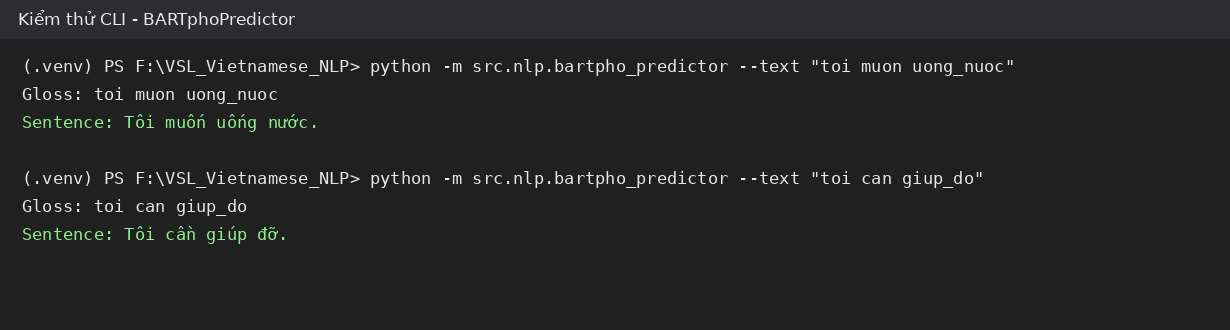
\includegraphics[width=0.78\textwidth]{figures/nlp/vsl_cli_prediction_examples.jpg}
\caption{Kiểm thử suy luận BARTpho bằng chuỗi gloss đầu vào}
\label{fig:vsl-cli-prediction-examples}
\end{figure}

\subsubsection{Khả năng tích hợp với pipeline realtime}

Mô-đun ghép câu được thiết kế để dễ tích hợp vào hệ thống thời gian thực:
\begin{itemize}
    \item giao diện đầu vào chỉ cần một chuỗi gloss đã chuẩn hóa;
    \item đầu ra là chuỗi văn bản thuần, có thể đưa tiếp sang mô-đun dịch hoặc hiển thị trực
    tiếp lên giao diện;
    \item có cơ chế suy giảm chất lượng mềm khi thiếu mô hình, thay vì dừng chương trình;
    \item logic được tách lớp rõ ràng, thuận tiện cho việc viết test riêng cho rule, model và
    fallback.
\end{itemize}

Về mặt phần mềm, đây là một quyết định quan trọng. Trong một pipeline nhiều mô-đun,
tầng NLP phải vừa đủ ``thông minh'' để cải thiện đầu ra, vừa đủ ``chắc'' để không phá vỡ
toàn bộ hệ thống khi môi trường triển khai chưa đầy đủ. Kiến trúc hiện tại đáp ứng tốt yêu
cầu đó và là nền tảng phù hợp để sau này nối trực tiếp với mô-đun nhận diện và mô-đun
dịch Việt - Lào.


\subsection{Xây dựng mô-đun dịch Việt - Lào}

Sau khi mô-đun ghép câu trả về câu tiếng Việt hoàn chỉnh, mô-đun dịch Việt - Lào tiếp
nhận chuỗi đó và thực hiện suy luận dịch máy. So với mô-đun ghép câu, phần cài đặt của
mô-đun dịch ngắn hơn, nhưng mỗi bước đều phụ thuộc chặt vào cấu hình của mô hình nền
đa ngôn ngữ và adapter LoRA.

\subsubsection{Các thành phần chính trong mã nguồn}

Trong snapshot hiện tại, mô-đun dịch được tổ chức khá gọn, trọng tâm nằm ở tệp
\texttt{translate.py}. Tệp này chịu trách nhiệm:
\begin{itemize}
    \item nạp tokenizer từ thư mục adapter;
    \item nạp mô hình nền \texttt{facebook/nllb-200-distilled-600M};
    \item ghép adapter LoRA bằng \texttt{PeftModel.from\_pretrained()};
    \item cung cấp hàm \texttt{translate\_vi\_to\_lao(text)} để suy luận;
    \item chạy giao diện dòng lệnh tối giản để thử dịch từng câu.
\end{itemize}

\begin{table}[H]
\centering
\caption{Các thành phần phần mềm chính của mô-đun dịch Việt - Lào}
\begin{tabularx}{\textwidth}{|>{\raggedright\arraybackslash}p{5.2cm}|X|}
\hline
\textbf{Thành phần} & \textbf{Chức năng} \\
\hline
\texttt{translate.py} & Khởi tạo tokenizer, mô hình nền, adapter LoRA và thực hiện suy luận dịch. \\
\hline
\codepath{model/.../adapter_config.json} & Lưu cấu hình LoRA như hạng thấp, dropout và các lớp mục tiêu. \\
\hline
\codepath{model/.../adapter_model.safetensors} & Chứa trọng số adapter đã được fine-tune cho cặp Việt -- Lào. \\
\hline
\codepath{dataset/vi_lo_dataset_split} & Lưu các tập train, validation, test ở dạng CSV. \\
\hline
\end{tabularx}
\end{table}

\subsubsection{Quy trình khởi tạo mô hình}

Khi chương trình bắt đầu, \texttt{translate.py} thực hiện ba bước nạp chính:
\begin{enumerate}
    \item nạp tokenizer từ thư mục adapter cục bộ;
    \item nạp mô hình nền NLLB-200 Distilled 600M;
    \item gắn adapter LoRA vào mô hình nền bằng PEFT.
\end{enumerate}

Việc tách mô hình thành \textit{base model} và \textit{adapter} có hai lợi ích rõ rệt:
\begin{itemize}
    \item giảm kích thước phần cần lưu trữ trong repository;
    \item cho phép thay adapter theo từng tác vụ mà không phải sao chép toàn bộ mô hình
    dịch nền.
\end{itemize}

Về mặt triển khai, đây là một kiến trúc rất phù hợp cho đồ án vì có thể tái sử dụng cùng một
mô hình nền NLLB cho nhiều tác vụ hoặc nhiều cặp ngôn ngữ khác nhau trong tương lai.

\subsubsection{Quy trình suy luận một câu dịch}

Hàm \texttt{translate\_vi\_to\_lao(text)} hiện thực hóa suy luận theo đúng logic của
NLLB:
\begin{itemize}
    \item đặt \texttt{tokenizer.src\_lang = "vie\_Latn"};
    \item mã hóa câu đầu vào thành tensor;
    \item gọi \texttt{model.generate()} với \texttt{forced\_bos\_token\_id} tương ứng
    \texttt{lao\_Laoo};
    \item giới hạn độ dài sinh ở 128 token;
    \item dùng \texttt{num\_beams = 5} để tăng độ ổn định của đầu ra;
    \item giải mã tensor sinh ra thành câu tiếng Lào.
\end{itemize}

Ý nghĩa của cấu hình này là mô hình luôn biết rõ ngôn ngữ nguồn và ngôn ngữ đích trong
quá trình suy luận. Với các mô hình dịch đa ngôn ngữ, đây là điều bắt buộc, vì thiếu token
ngôn ngữ sẽ dễ dẫn đến đầu ra sai ngôn ngữ hoặc pha trộn mã ngôn ngữ không mong muốn.

\begin{figure}[H]
\centering
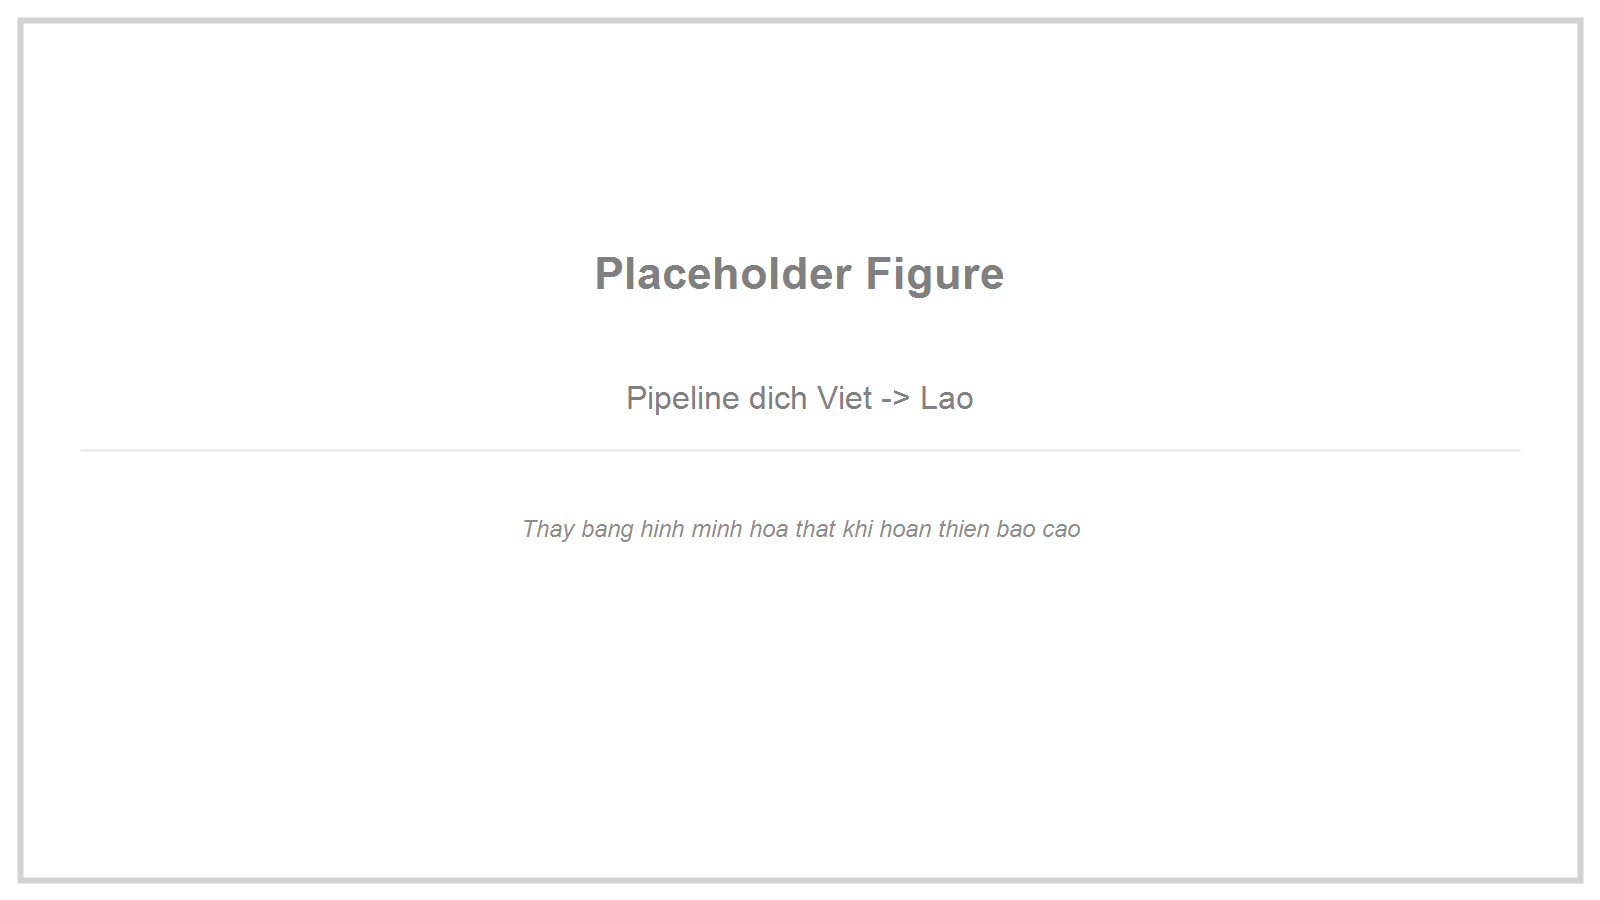
\includegraphics[width=0.86\textwidth]{figures/translation/vi_lao_mt_pipeline.png}
\caption{Luồng cài đặt và suy luận trong mô-đun dịch Việt -- Lào}
\label{fig:translation-runtime}
\end{figure}

\subsubsection{Vai trò của LoRA trong phần mềm}

Mặc dù phần mã gọi LoRA chỉ gồm vài dòng, adapter thực chất là thành phần quan trọng
nhất quyết định việc mô hình nền NLLB có thích nghi được với cặp Việt - Lào hay không.
Trong project này, LoRA được gắn vào các lớp attention projection và lớp đầu ra, tức là
đúng những điểm có ảnh hưởng mạnh đến khả năng căn chỉnh biểu diễn giữa câu nguồn và
câu đích.

So với full fine-tuning, cách làm này mang lại ba lợi ích trực tiếp cho phần mềm:
\begin{itemize}
    \item dễ đóng gói mô hình hơn;
    \item ít rủi ro hơn khi cập nhật mô hình nền;
    \item thuận tiện cho việc thử nhiều adapter khác nhau trên cùng một interface dịch.
\end{itemize}

\subsubsection{Tích hợp với mô-đun ghép câu phía trước}

Mô-đun dịch chỉ thực sự phát huy hiệu quả khi câu tiếng Việt đầu vào đã đủ mạch lạc. Vì
vậy, chất lượng của mô-đun này phụ thuộc mạnh vào đầu ra của mô-đun ghép câu:
\begin{itemize}
    \item nếu câu tiếng Việt rõ chủ-vị và đúng ý nghĩa, NLLB dễ dịch chính xác hơn;
    \item nếu câu tiếng Việt còn thiếu thành phần, dịch máy dễ tạo ra câu tiếng Lào khó
    hiểu hoặc lệch nghĩa;
    \item nếu tầng ghép câu đã chuẩn hóa dấu câu và viết hoa, tokenizer của mô hình dịch
    cũng làm việc ổn định hơn.
\end{itemize}

Nói cách khác, hai mô-đun NLP trong hệ thống không tách rời, mà bổ trợ cho nhau theo
kiểu nối tầng: mô-đun ghép câu giảm nhiễu ngôn ngữ nội bộ, còn mô-đun dịch chuyển ý
nghĩa đó sang ngôn ngữ đích.

\subsubsection{Nhận xét về hiện thực phần mềm}

Điểm mạnh của phần cài đặt hiện tại là đơn giản, rõ ràng và đúng với thực tế nghiên cứu
ứng dụng. Chỉ với một script ngắn, hệ thống đã có thể nạp được mô hình nền đa ngôn ngữ,
adapter tinh chỉnh riêng cho tác vụ và thực hiện suy luận câu mới.

Tuy nhiên, vẫn còn các điểm cần hoàn thiện thêm trong giai đoạn sau:
\begin{itemize}
    \item chưa có script đánh giá full test set đi kèm trực tiếp trong snapshot hiện tại;
    \item chưa có lớp giao tiếp trung gian để gọi mô-đun dịch như một service trong ứng
    dụng lớn hơn;
    \item lần chạy đầu tiên có thể phụ thuộc vào việc mô hình nền đã có cache cục bộ hay
    chưa.
\end{itemize}

Những điểm này không làm sai kiến trúc của mô-đun, nhưng là các hạng mục nên được bổ
sung nếu muốn biến phần nghiên cứu thành sản phẩm phần mềm hoàn chỉnh hơn.


\subsection{Tích hợp pipeline thời gian thực}

Sau khi từng mô-đun hoạt động độc lập, bước tiếp theo là ghép chúng thành một pipeline thời gian thực. Trong repository hiện tại, script \texttt{realtime\_integrated.py} đảm nhiệm vai trò điều phối: gọi mô-đun nhận diện theo luồng webcam, quản lý token buffer, gọi mô-đun ghép câu tiếng Việt và tùy chọn gọi mô-đun dịch Việt -- Lào.

Vòng lặp realtime gồm các bước chính:
\begin{enumerate}
    \item đọc frame từ webcam và đưa qua mô-đun nhận diện ASL-250;
    \item hiển thị top-k dự đoán hiện tại để người vận hành quan sát;
    \item khi nhấn \texttt{a}, lấy top-1 prediction hiện tại, ánh xạ sang token tiếng Việt và thêm vào buffer;
    \item khi nhấn \texttt{b}, gửi buffer sang \texttt{SentenceBuilder} để sinh câu tiếng Việt, sau đó dịch sang tiếng Lào nếu không chạy ở chế độ \texttt{--no-translation};
    \item khi nhấn \texttt{c}, xóa token buffer để bắt đầu câu mới;
    \item khi nhấn \texttt{SPACE}, reset bộ đệm frame của mô-đun nhận diện;
    \item khi nhấn \texttt{q}, thoát chương trình và giải phóng camera.
\end{enumerate}

Thiết kế này có ưu điểm là đơn giản, dễ quan sát và phù hợp cho demo học thuật. Người vận hành có thể kiểm soát thời điểm thêm token, thời điểm ghép câu và thời điểm dịch, nhờ đó giảm rủi ro do mô hình nhận diện nhảy nhãn trong vài frame ngắn. Khi mô hình dịch chưa được tải hoặc máy không đủ tài nguyên, tùy chọn \texttt{--no-translation} giúp kiểm thử hai tầng đầu mà không làm gián đoạn toàn bộ pipeline.


\subsection{Giao diện chạy thử và các đoạn mã tiêu biểu}

Phần giao diện chạy thử tập trung vào tính quan sát được của pipeline. Khi chương trình realtime hoạt động, màn hình cần thể hiện tối thiểu ba nhóm thông tin: khung hình webcam kèm skeleton/landmarks, top-k nhãn nhận diện hiện tại và trạng thái buffer/câu đầu ra. Cách hiển thị này giúp người vận hành biết mô hình đang nhìn thấy gì, đang dự đoán nhãn nào và dữ liệu nào sẽ được đưa sang tầng NLP.

\begin{itemize}
    \item Khung video hiển thị người dùng, skeleton pose và landmarks bàn tay do MediaPipe vẽ.
    \item Vùng dự đoán hiển thị top-3 nhãn ký hiệu cùng xác suất tương ứng.
    \item Vùng buffer hiển thị các token đã được xác nhận bằng phím \texttt{a}.
    \item Vùng kết quả hiển thị câu tiếng Việt sau khi nhấn \texttt{b} và câu tiếng Lào nếu bật mô-đun dịch.
\end{itemize}

Các đoạn mã nên đưa vào báo cáo chỉ cần đại diện cho logic chính, chẳng hạn hàm ánh xạ nhãn ASL sang token tiếng Việt, thao tác thêm token vào buffer và lời gọi ghép câu/dịch. Phần code dài như khởi tạo MediaPipe, nạp TensorFlow Lite Interpreter hoặc cấu hình NLLB nên được mô tả bằng lời trong thân báo cáo để tránh làm loãng nội dung kỹ thuật chính.



\clearpage


\section{THỰC NGHIỆM, ĐÁNH GIÁ, KẾT LUẬN VÀ HƯỚNG PHÁT TRIỂN}

\subsection{Thiết lập thực nghiệm}

Thiết lập thực nghiệm cần được mô tả rõ để các kết quả đánh giá được hiểu đúng bối cảnh. Do hệ thống gồm ba mô-đun có bản chất khác nhau, phần đánh giá được tách thành bốn nhóm: nhận diện ký hiệu, khôi phục câu tiếng Việt, dịch Việt -- Lào và đánh giá tích hợp end-to-end.

Trong snapshot hiện tại, mô-đun nhận diện sử dụng mô hình TFLite pre-trained nên không có log huấn luyện riêng trong repository. Nhóm bổ sung script đánh giá riêng để đo latency và tính Top-k Accuracy, Precision, Recall, F1 khi có tập landmarks/video gán nhãn; tuy nhiên workspace hiện chưa có test manifest gán nhãn cho tầng nhận diện nên không công bố số accuracy/F1 tự suy diễn. Mô-đun khôi phục câu tiếng Việt có báo cáo đánh giá trên tập test của bộ dữ liệu VSL Vietnamese NLP. Mô-đun dịch Việt -- Lào có dữ liệu train/validation/test và adapter LoRA; các chỉ số Train loss, Validation loss và BLEU được trích từ tài liệu \texttt{vilo.pdf}. Các metric chrF và TER chưa thấy số liệu truy vết trong workspace nên không được tự suy diễn.

\begin{table}[H]
\centering
\caption{Môi trường và dữ liệu dùng trong thực nghiệm}
\label{tab:experiment-setup}
\begin{tabularx}{\textwidth}{|l|X|}
\hline
\textbf{Thành phần} & \textbf{Mô tả} \\
\hline
Thiết bị demo & Máy tính Windows có webcam; mô-đun nhận diện chạy bằng TensorFlow Lite/MediaPipe trên CPU trong chế độ demo. \\
\hline
Mô-đun nhận diện & Mô hình \texttt{model.tflite} từ Kaggle ASL Signs, 250 lớp, đầu vào 543 landmarks x 3 tọa độ, cửa sổ 16--60 frame. \\
\hline
Mô-đun tiếng Việt & BARTpho kết hợp rule/fallback; dữ liệu chính gồm 32.755 cặp gloss -- câu tiếng Việt, chia train/validation/test. \\
\hline
Mô-đun dịch & NLLB-200 Distilled 600M kết hợp adapter LoRA; dữ liệu song ngữ Việt -- Lào gồm 100.000 cặp câu, chia 90.000/5.000/5.000. \\
\hline
Thư viện chính & Python, OpenCV, MediaPipe, TensorFlow Lite, PyTorch, Transformers, PEFT, SentencePiece. \\
\hline
\end{tabularx}
\end{table}

Để tránh trộn lẫn kết quả giữa các tầng, mỗi mô-đun được đánh giá theo đúng đầu vào chuẩn của nó. Tầng nhận diện được đánh giá bằng latency TFLite và quan sát webcam; Top-k Accuracy, Macro F1 và confusion matrix được xác định là metric bắt buộc khi có tập video/landmark gán nhãn riêng. Tầng tiếng Việt được đánh giá bằng loss, perplexity, Exact Match, BLEU, ROUGE-L, chrF và Token F1. Tầng dịch được đề xuất đánh giá bằng BLEU, chrF, TER và kiểm tra thủ công về adequacy/fluency. Đánh giá end-to-end tập trung vào độ đúng của câu cuối cùng, độ trễ và khả năng vận hành ổn định khi chạy liên tục.


\subsection{Đánh giá mô hình nhận diện ký hiệu}

Mô-đun nhận diện là tầng đầu tiên của toàn bộ pipeline nên mọi sai số ở đây đều có thể lan xuống mô-đun
ghép câu và mô-đun dịch. Vì mô hình hiện tại là một mô hình pre-trained (TFLite từ cuộc thi Kaggle
ASL Signs), cách đánh giá sẽ khác so với một mô hình tự huấn luyện: nhóm không có quá trình
training/validation thông thường, mà tập trung vào đánh giá chất lượng suy luận thực tế.

\subsubsection{Các metric có thể đánh giá}

Mặc dù mô hình nhận diện trong đề tài là mô hình pre-trained, mô-đun này vẫn cần được đánh giá như
một bộ phân loại đa lớp. Điểm khác biệt là nhóm không báo cáo loss huấn luyện hay validation loss do
không huấn luyện lại mô hình; thay vào đó, phần đánh giá tập trung vào chất lượng dự đoán trên tập
kiểm thử gán nhãn và tốc độ suy luận. Các metric phù hợp bao gồm:
\begin{itemize}
    \item \textbf{Top-1 Accuracy}: tỉ lệ dự đoán đúng nhãn ký hiệu trên tập kiểm thử;
    \item \textbf{Top-3/Top-5 Accuracy}: tỉ lệ nhãn đúng nằm trong top-k dự đoán;
    \item \textbf{Macro Precision, Macro Recall, Macro F1}: đánh giá cân bằng theo từng lớp, tránh việc
    một vài lớp xuất hiện nhiều làm sai lệch kết quả chung;
    \item \textbf{Weighted F1}: F1 có trọng số theo số mẫu của từng lớp;
    \item \textbf{Confusion matrix}: ma trận nhầm lẫn giữa các lớp ký hiệu;
    \item \textbf{Average inference time}: thời gian suy luận trung bình trên mỗi chuỗi landmarks;
    \item \textbf{FPS}: số khung hình xử lý được trong một giây, quan trọng cho demo realtime;
    \item \textbf{Đánh giá định tính}: quan sát trực tiếp khi sử dụng webcam.
\end{itemize}

\begin{table}[H]
\centering
\caption{Ý nghĩa của các metric cho mô-đun nhận diện}
\label{tab:recognition-metric-meanings}
\begin{tabularx}{\textwidth}{|p{3cm}|X|X|}
\hline
\textbf{Metric} & \textbf{Ý nghĩa} & \textbf{Cách diễn giải} \\
\hline
Top-1 Accuracy & Tỉ lệ mẫu có lớp dự đoán cao nhất trùng đúng nhãn thật. & Càng cao càng tốt; là chỉ số chính của bài toán phân loại. \\
\hline
Top-3 Accuracy & Tỉ lệ mẫu mà nhãn thật xuất hiện trong 3 dự đoán cao nhất. & Hữu ích khi số lớp lớn và nhiều dấu hiệu gần nhau. \\
\hline
Top-5 Accuracy & Tỉ lệ mẫu mà nhãn thật xuất hiện trong 5 dự đoán cao nhất. & Cho thấy mô hình có ``nhìn ra'' vùng ứng viên đúng hay không. \\
\hline
Macro F1 & Trung bình F1 theo từng lớp ký hiệu. & Phù hợp khi muốn xem mô hình có công bằng giữa các lớp hay không. \\
\hline
Confusion matrix & Bảng đếm nhãn thật và nhãn dự đoán. & Dùng để phát hiện các cặp ký hiệu dễ bị nhầm. \\
\hline
Latency / FPS & Tốc độ suy luận trên mỗi mẫu hoặc theo khung hình. & Quyết định khả năng dùng trong realtime demo. \\
\hline
\end{tabularx}
\end{table}

Với tập kiểm thử gồm $N$ mẫu, nhãn thật $y_i$ và danh sách dự đoán top-k là $\hat{Y}_{i,k}$, các chỉ số
Top-k Accuracy được tính như sau:
\[
    TopK = \frac{1}{N}\sum_{i=1}^{N}\mathbf{1}(y_i \in \hat{Y}_{i,k})
\]

Precision, Recall và F1 theo từng lớp được tính từ số lượng true positive ($TP$), false positive ($FP$)
và false negative ($FN$):
\[
    Precision = \frac{TP}{TP + FP}, \quad
    Recall = \frac{TP}{TP + FN}, \quad
    F1 = \frac{2 \times Precision \times Recall}{Precision + Recall}
\]

\subsubsection{Bối cảnh mô hình pre-trained}

Cần nhấn mạnh rằng mô hình TFLite trong dự án là giải pháp đạt giải nhất cuộc thi Kaggle
\textit{Google -- Isolated Sign Language Recognition}. Cuộc thi này có hơn 1.000 đội tham gia
và đánh giá trên dữ liệu kiểm thử chính thức của Kaggle. Vì vậy, chất lượng của mô hình đã được
kiểm chứng ở quy mô cạnh tranh quốc tế.

Tuy nhiên, kết quả trong cuộc thi Kaggle được đo trên dữ liệu landmarks đã chuẩn bị sẵn, trong khi
pipeline thực tế của dự án phải trích xuất landmarks từ webcam theo thời gian thực. Điều này có thể
tạo ra chênh lệch giữa chất lượng offline (trên dữ liệu Kaggle) và chất lượng online (trên webcam
thực tế), do:
\begin{itemize}
    \item chất lượng camera, ánh sáng và nền ảnh hưởng đến độ chính xác của MediaPipe;
    \item tốc độ ký hiệu và khoảng cách tới camera có thể khác so với điều kiện trong dữ liệu
    huấn luyện;
    \item một số từ vựng trong 250 lớp có thể gần nhau về hình thức, dễ gây nhầm.
\end{itemize}

\begin{table}[H]
\centering
\caption{Thông tin tham chiếu từ cuộc thi Kaggle ASL Signs}
\label{tab:kaggle-asl-reference}
\begin{tabularx}{\textwidth}{|X|c|}
\hline
\textbf{Thuộc tính} & \textbf{Giá trị} \\
\hline
Tên cuộc thi & Google -- Isolated Sign Language Recognition \\
\hline
Số lớp từ vựng & 250 \\
\hline
Nguồn mô hình & Giải pháp đạt giải nhất (1st place solution) \\
\hline
Định dạng & TensorFlow Lite (.tflite) \\
\hline
Kích thước mô hình & $\sim$11 MB \\
\hline
\end{tabularx}
\end{table}

\subsubsection{Công cụ đánh giá định lượng}

Để phần nhận diện không chỉ dừng ở mức ``chạy mô hình pre-trained'', nhóm bổ sung script
\codepath{external/asl_baseline/evaluate_asl_250.py}. Script này có hai chế độ:
\begin{itemize}
    \item \textbf{benchmark-only}: đo thời gian suy luận của mô hình TFLite trên tensor landmarks giả lập
    có đúng kích thước đầu vào \texttt{N x 543 x 3};
    \item \textbf{manifest evaluation}: đọc file CSV gồm hai cột \texttt{path,label}, chạy suy luận trên
    các file landmarks \texttt{.npy}/\texttt{.npz}, sau đó xuất Top-1, Top-3, Top-5 Accuracy, Macro
    Precision, Macro Recall, Macro F1, Weighted F1, latency và confusion matrix.
\end{itemize}

Lệnh benchmark tốc độ đã dùng trong snapshot này:
\begin{verbatim}
venv\Scripts\python.exe external\google-asl-250\evaluate_asl_250.py ^
  --benchmark-only --runs 30 --warmup 5
\end{verbatim}

Khi có tập kiểm thử landmarks gán nhãn, lệnh đánh giá phân loại có dạng:
\begin{verbatim}
venv\Scripts\python.exe external\google-asl-250\evaluate_asl_250.py ^
  --manifest test_manifest.csv --output-dir external\google-asl-250\eval_results
\end{verbatim}

\begin{table}[H]
\centering
\caption{Kết quả benchmark suy luận TFLite của mô-đun nhận diện}
\label{tab:recognition-latency-benchmark}
\begin{tabularx}{\textwidth}{|c|c|c|c|}
\hline
\textbf{Độ dài chuỗi} & \textbf{Mean latency (ms)} & \textbf{P95 latency (ms)} & \textbf{FPS tương đương} \\
\hline
16 frame & 13,26 & 16,57 & 75,40 \\
\hline
32 frame & 26,26 & 36,91 & 38,09 \\
\hline
60 frame & 44,92 & 49,92 & 22,26 \\
\hline
\end{tabularx}
\end{table}

Các số liệu trong Bảng~\ref{tab:recognition-latency-benchmark} chỉ đo phần suy luận TFLite trên CPU,
chưa bao gồm thời gian đọc webcam, tiền xử lý ảnh và trích xuất landmarks bằng MediaPipe. Tuy vậy, kết
quả này cho thấy riêng mô hình phân loại đủ nhanh để phục vụ demo realtime, vì trong code hiện tại mô
hình chỉ được gọi mỗi 8 frame thay vì gọi ở mọi frame.

\begin{table}[H]
\centering
\caption{Trạng thái các metric phân loại của mô-đun nhận diện trong snapshot hiện tại}
\label{tab:recognition-classification-status}
\begin{tabularx}{\textwidth}{|p{4cm}|p{3.2cm}|X|}
\hline
\textbf{Metric} & \textbf{Trạng thái} & \textbf{Ghi chú} \\
\hline
Top-1 Accuracy & Chưa công bố số & Cần tập kiểm thử landmarks/video có nhãn thật. Repository hiện chỉ có mô hình pre-trained và label map, chưa có test manifest cho recognition. \\
\hline
Top-3 / Top-5 Accuracy & Chưa công bố số & Script đã hỗ trợ tính tự động khi có dữ liệu gán nhãn. \\
\hline
Macro Precision / Recall / F1 & Chưa công bố số & Không thể tính đúng nếu thiếu \texttt{y\_true}. Việc tự đưa số khi chưa có tập test sẽ không có giá trị học thuật. \\
\hline
Confusion matrix & Chưa công bố bảng & Sẽ được xuất ra file \texttt{recognition\_confusion\_matrix.csv} khi chạy đánh giá với manifest gán nhãn. \\
\hline
Latency / FPS & Đã đo & Có số liệu benchmark TFLite trong Bảng~\ref{tab:recognition-latency-benchmark}. \\
\hline
\end{tabularx}
\end{table}

\subsubsection{Đánh giá thực nghiệm qua demo realtime}

Vì snapshot hiện tại chưa có tập test nhận diện riêng, phần đánh giá thực nghiệm qua webcam được dùng
để kiểm tra khả năng vận hành thực tế của pipeline. Đây không thay thế cho Top-k Accuracy hay F1, nhưng
có giá trị bổ sung vì pipeline thật phải đi qua camera, MediaPipe và cửa sổ trượt thời gian. Các tiêu
chí đánh giá bao gồm:
\begin{itemize}
    \item mô hình có nhận đúng các từ vựng phổ biến như \texttt{hello}, \texttt{drink},
    \texttt{food}, \texttt{please}, \texttt{thankyou} hay không;
    \item mô hình phản hồi nhanh bao lâu sau khi người dùng bắt đầu ký hiệu;
    \item mô hình có ổn định (không nhảy liên tục giữa các nhãn) khi người dùng giữ tay
    trong tư thế;
    \item mô hình xử lý thế nào khi người dùng chuyển giữa các ký hiệu liên tiếp.
\end{itemize}

\begin{table}[H]
\centering
\caption{Đánh giá định tính mô-đun nhận diện qua webcam}
\label{tab:recognition-qualitative}
\begin{tabularx}{\textwidth}{|X|p{3.2cm}|X|}
\hline
\textbf{Kịch bản thử nghiệm} & \textbf{Kết quả} & \textbf{Nhận xét} \\
\hline
Ký hiệu từ phổ biến như \texttt{hello}, \texttt{drink} & Hoạt động được trong demo & Các nhãn phổ biến có thể xuất hiện ổn định hơn khi tay nằm rõ trong khung hình và ánh sáng đủ. \\
\hline
Ký hiệu liên tiếp nhiều từ & Cần xác nhận từng token & Phiên bản hiện tại phù hợp hơn với cơ chế chọn token/top-1 vào buffer, chưa phải nhận diện câu liên tục hoàn toàn tự động. \\
\hline
Điều kiện ánh sáng yếu & Dễ giảm ổn định & MediaPipe có thể mất landmarks tay hoặc pose, kéo theo dự đoán TFLite kém tin cậy. \\
\hline
Tốc độ ký hiệu nhanh & Có thể bỏ sót động tác & Cửa sổ trượt cần đủ tối thiểu 16 frame; thao tác quá nhanh làm chuỗi landmarks thiếu ngữ cảnh. \\
\hline
Khoảng cách xa camera & Dễ mất chi tiết bàn tay & Khi bàn tay quá nhỏ hoặc bị che, landmarks không ổn định và xác suất dự đoán dao động mạnh. \\
\hline
\end{tabularx}
\end{table}

\subsubsection{Đánh giá định tính và phân tích lỗi}

Bên cạnh các quan sát trực tiếp, phần nhận diện cần có thêm phân tích lỗi theo các hướng:
\begin{itemize}
    \item \textbf{nhầm lớp do động tác gần giống}: nhiều từ khác nhau chỉ lệch hướng cổ tay hoặc biên
    độ chuyển động;
    \item \textbf{nhầm do điều kiện ghi hình}: ánh sáng yếu, nền lộn xộn, tay che nhau hoặc ra ngoài
    khung hình;
    \item \textbf{nhầm do sự khác biệt signer}: mô hình được huấn luyện trên signer trong dữ liệu
    Kaggle, có thể chưa khái quát tốt cho người dùng thực tế;
    \item \textbf{giới hạn 250 từ}: nếu người dùng thực hiện ký hiệu không nằm trong 250 lớp,
    mô hình sẽ dự đoán sai.
\end{itemize}

\subsubsection{Lưu ý khi diễn giải kết quả}

Ngay cả khi mô hình nhận diện hoạt động tốt, vẫn cần nhấn mạnh rằng:
\begin{itemize}
    \item đây mới là chất lượng ở tầng phân loại gloss, chưa phải chất lượng câu tiếng Việt hay tiếng
    Lào cuối cùng;
    \item mô hình được huấn luyện trên dữ liệu ASL, nên kết quả tốt không đồng nghĩa mô hình
    đã ``hiểu'' trọn vẹn VSL thật trong thực địa;
    \item cần tách bạch rõ \textit{recognition accuracy}, \textit{sentence quality}
    và \textit{translation quality}, thay vì gộp chung thành một đánh giá mơ hồ.
\end{itemize}

Trình bày như vậy vừa chính xác về mặt học thuật, vừa giúp người đọc hiểu đúng đóng góp thật của mô
hình nhận diện trong toàn bộ hệ thống.


\subsection{Đánh giá mô hình khôi phục câu tiếng Việt}

Mô-đun ghép câu tiếng Việt là một bài toán sinh văn bản có cấu trúc. Vì vậy, nếu chỉ dùng
một metric duy nhất sẽ khó phản ánh đầy đủ chất lượng đầu ra. Trong báo cáo này, phần
đánh giá cần kết hợp cả \textit{metric huấn luyện} và \textit{metric tương đồng văn bản}:
\begin{itemize}
    \item \textbf{Loss} và \textbf{Perplexity} phản ánh mô hình học phân phối token tốt đến
    mức nào;
    \item \textbf{Exact Match} đo tỉ lệ câu dự đoán trùng hoàn toàn với câu tham chiếu;
    \item \textbf{BLEU} đo mức trùng khớp n-gram sửa đổi giữa câu sinh ra và câu chuẩn;
    \item \textbf{ROUGE-L} nhấn mạnh chuỗi con chung dài nhất, phù hợp khi muốn nhìn cấu
    trúc câu;
    \item \textbf{chrF} đo mức tương đồng ở cấp ký tự, hữu ích với tiếng Việt vì còn liên quan
    tới dấu và biến thể chính tả;
    \item \textbf{Token F1} và \textbf{Similarity Ratio} giúp nhìn thêm ở mức từ và mức chuỗi
    tổng quát.
\end{itemize}

Việc dùng đồng thời các metric trên là phù hợp với các nghiên cứu \textit{Gloss-to-Text}
gần đây, nơi người ta thường không chỉ báo cáo BLEU mà còn bổ sung ROUGE và chrF để
đánh giá nhiều khía cạnh của câu sinh ra.

\subsubsection{Ý nghĩa của từng nhóm metric}

\begin{table}[H]
\centering
\caption{Ý nghĩa của các metric dùng cho mô-đun ghép câu tiếng Việt}
\begin{tabularx}{\textwidth}{|p{3cm}|X|X|}
\hline
\textbf{Metric} & \textbf{Ý nghĩa} & \textbf{Cách diễn giải} \\
\hline
Test Loss & Sai số trung bình khi dự đoán token trên tập test. & Càng thấp càng tốt. \\
\hline
Perplexity & Độ khó dự đoán chuỗi đích của mô hình. & Càng gần 1 càng tốt. \\
\hline
Exact Match & Tỉ lệ câu dự đoán trùng hoàn toàn với câu chuẩn. & Phản ánh độ đúng tuyệt đối. \\
\hline
BLEU & Độ trùng n-gram giữa câu sinh ra và câu tham chiếu. & Phản ánh mức gần giống ở cấp cụm từ. \\
\hline
ROUGE-L & Độ dài chuỗi con chung dài nhất giữa hai câu. & Hữu ích khi quan tâm cấu trúc câu. \\
\hline
chrF & Độ giống nhau ở cấp ký tự. & Nhạy với dấu tiếng Việt và lỗi chính tả nhỏ. \\
\hline
Token F1 & Độ trùng token giữa dự đoán và tham chiếu. & Cân bằng precision và recall theo từ. \\
\hline
Similarity Ratio & Độ tương đồng chuỗi ở mức tổng quát. & Hỗ trợ nhìn nhanh mức độ gần giống. \\
\hline
\end{tabularx}
\end{table}

\begin{figure}[H]
\centering
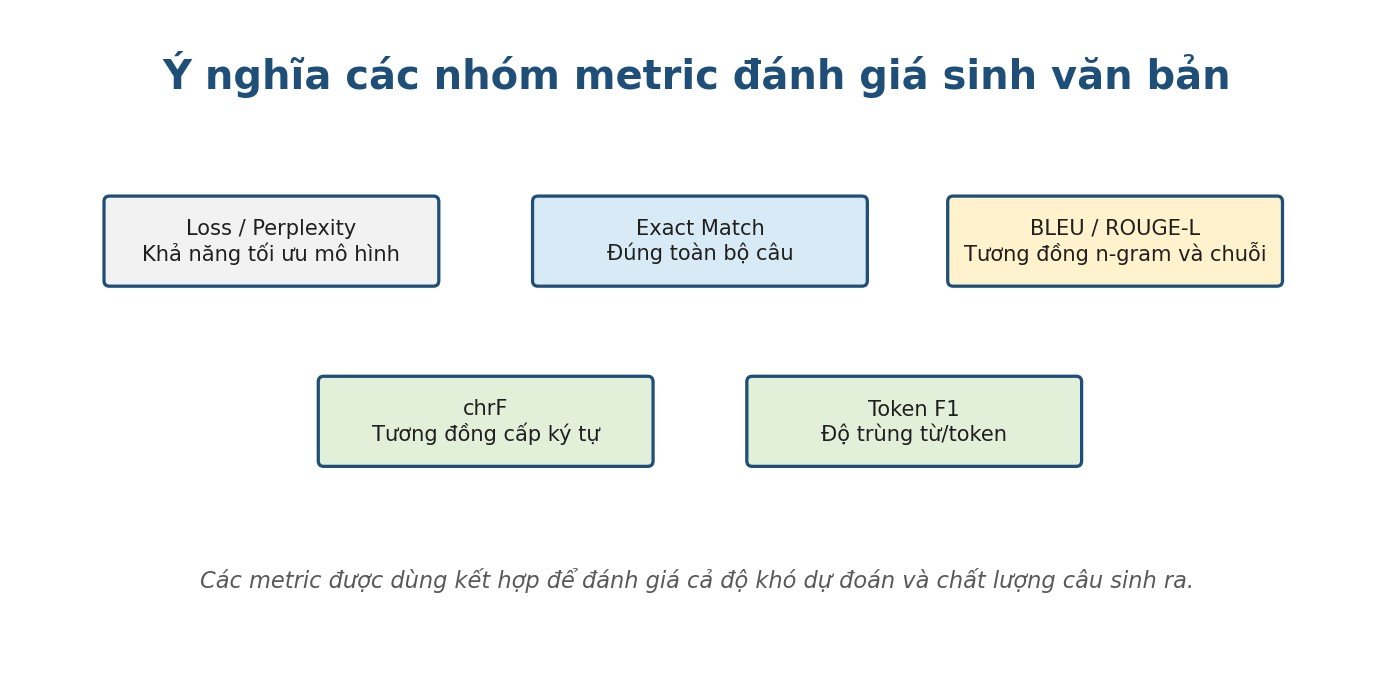
\includegraphics[width=0.82\textwidth]{figures/nlp/vsl_metric_groups.jpg}
\caption{Nhóm ý nghĩa của các metric đánh giá sinh văn bản}
\label{fig:vsl-metric-groups}
\end{figure}

\subsubsection{Kết quả thực nghiệm trên tập test}

Theo báo cáo kỹ thuật của mô-đun \texttt{VSL\_Vietnamese\_NLP}, BARTpho được đánh giá
trên 3.276 mẫu của tập test và cho kết quả như Bảng~\ref{tab:vietnamese-nlp-results}.
Các số liệu này được lấy trực tiếp từ thư mục output của project:
\codepath{VSL_Vietnamese_NLP/outputs/reports/bartpho_sentence_reports/}. Trong đó,
\codepath{bartpho_sentence_metrics_full.json} lưu metric tổng hợp,
\codepath{bartpho_sentence_predictions_full.csv} lưu toàn bộ dự đoán trên tập test và
\codepath{bartpho_sentence_sample_predictions_full.txt} lưu các mẫu dự đoán dễ đọc. Các
giá trị metric này cũng trùng với phần đánh giá trong tài liệu \texttt{vsl.pdf}, mục kết quả
BARTpho trên tập test của module ghép gloss thành câu tiếng Việt.

\begin{table}[H]
\centering
\caption{Kết quả đánh giá mô-đun ghép câu tiếng Việt trên tập test}
\label{tab:vietnamese-nlp-results}
\begin{tabularx}{\textwidth}{|X|c|}
\hline
\textbf{Metric} & \textbf{Giá trị} \\
\hline
Số mẫu test & 3.276 \\
\hline
Test Loss & 0,0040 \\
\hline
Perplexity & 1,0040 \\
\hline
Exact Match & 0,9942 \\
\hline
BLEU & 99,7848 \\
\hline
ROUGE-L & 0,9990 \\
\hline
chrF & 99,8693 \\
\hline
Token F1 & 0,9980 \\
\hline
Similarity Ratio & 0,9991 \\
\hline
\textbf{Exact Match đúng/sai} & \textbf{3.257 / 19} \\
\hline
\end{tabularx}
\end{table}

\begin{figure}[H]
\centering
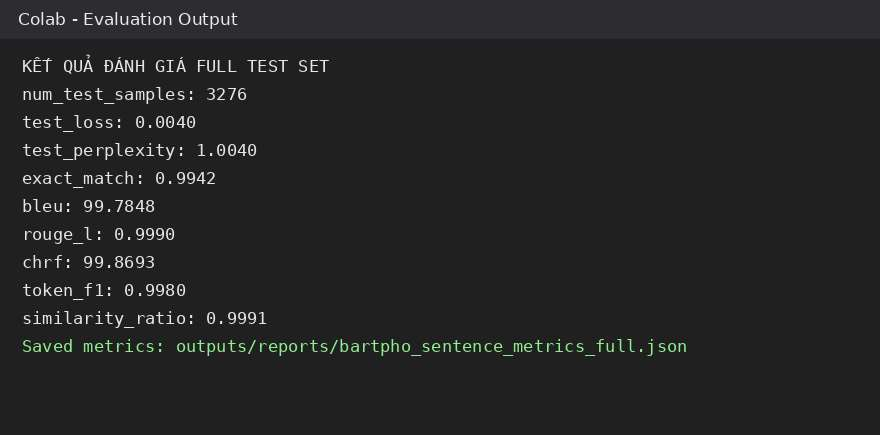
\includegraphics[width=0.78\textwidth]{figures/nlp/vsl_full_test_output.jpg}
\caption{Kết quả đánh giá tự động trên toàn bộ tập test}
\label{fig:vsl-full-test-output}
\end{figure}

\begin{figure}[H]
\centering
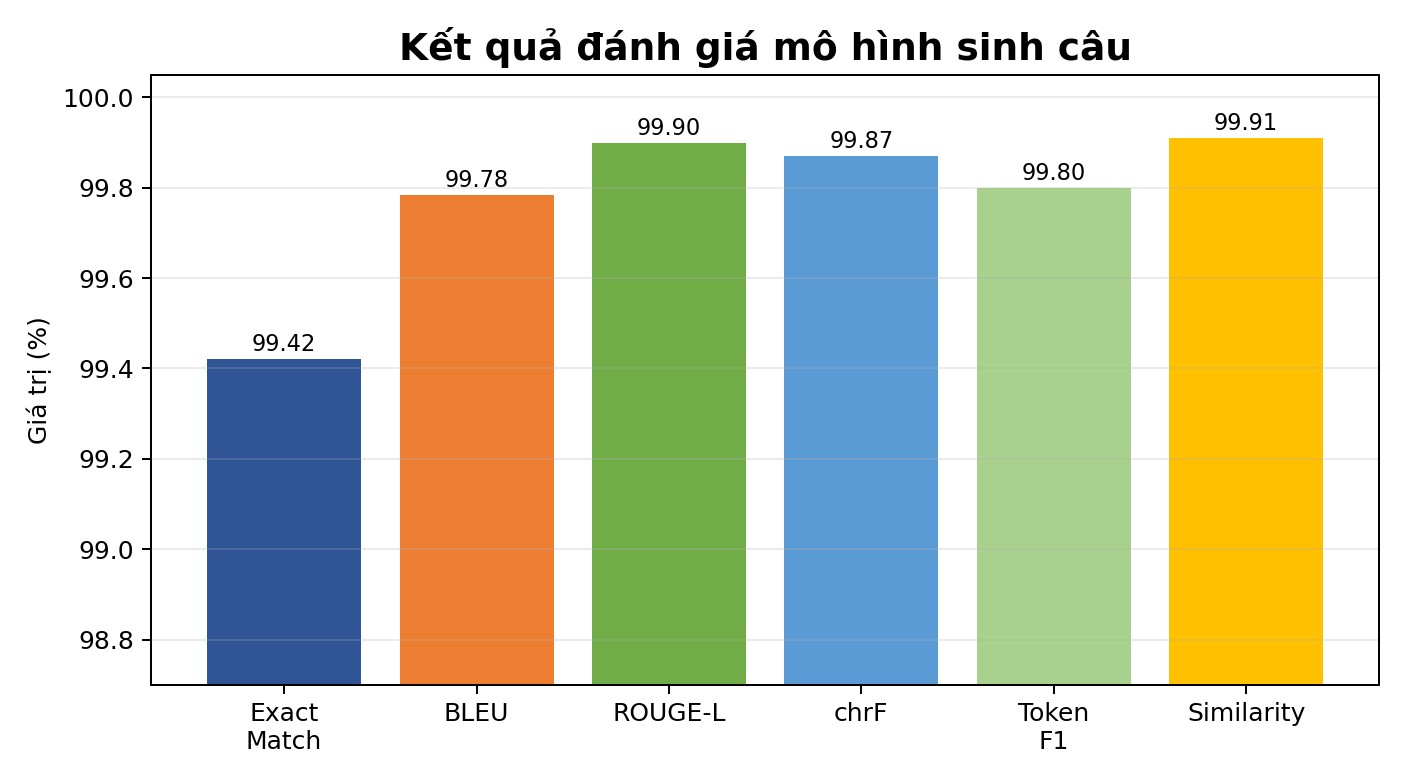
\includegraphics[width=0.9\textwidth]{figures/nlp/vsl_bartpho_metrics_chart.jpg}
\caption{Biểu đồ các metric đánh giá BARTpho trên tập test}
\label{fig:vsl-bartpho-metrics-chart}
\end{figure}

\begin{figure}[H]
\centering
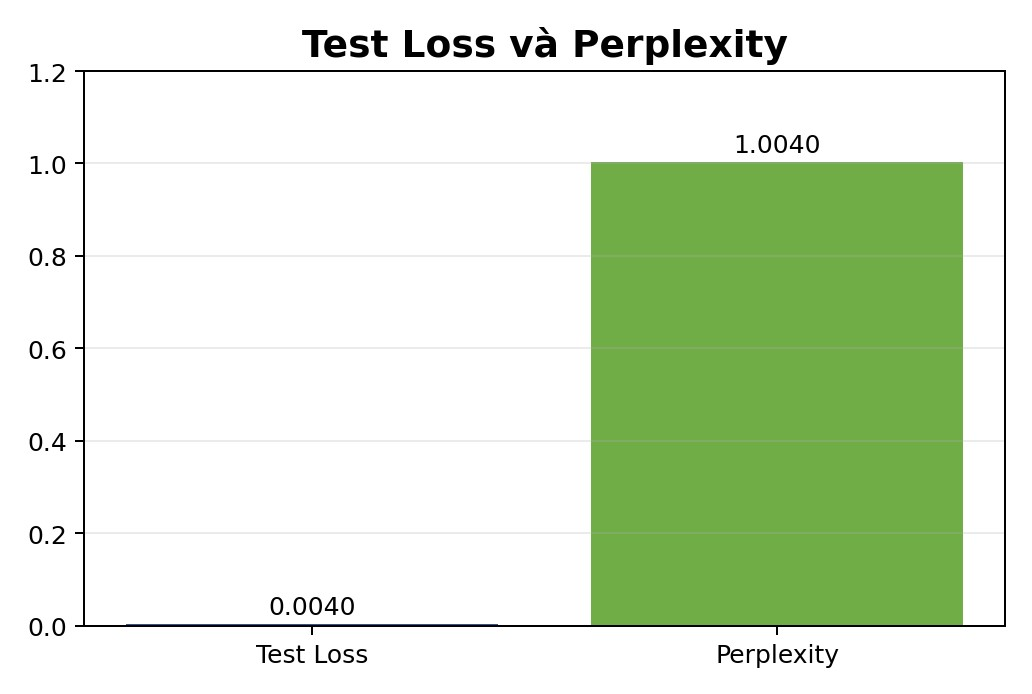
\includegraphics[width=0.72\textwidth]{figures/nlp/vsl_bartpho_loss_perplexity_chart.jpg}
\caption{Biểu đồ Test Loss và Perplexity của BARTpho}
\label{fig:vsl-bartpho-loss-perplexity-chart}
\end{figure}

\subsubsection{Phân tích kết quả}

Các con số trên cho thấy mô hình hoạt động rất tốt trên bộ test hiện tại. Có thể rút ra một
số nhận xét chính:
\begin{itemize}
    \item \textbf{Exact Match = 0,9942} cho thấy gần như toàn bộ câu dự đoán trùng hoàn
    toàn với câu chuẩn. Với một tác vụ có miền dữ liệu giao tiếp tương đối hẹp, đây là tín
    hiệu rất mạnh cho thấy mô hình đã học tốt cấu trúc ánh xạ từ gloss sang câu.
    \item \textbf{BLEU = 99,7848} và \textbf{ROUGE-L = 0,9990} cho thấy câu sinh ra gần
    như trùng khớp hoàn toàn với câu tham chiếu cả ở mức n-gram lẫn cấu trúc chuỗi.
    \item \textbf{chrF = 99,8693} đặc biệt quan trọng với tiếng Việt vì chứng tỏ mô hình giữ
    được dấu và hình thức ký tự rất tốt.
    \item \textbf{Perplexity = 1,0040} cho thấy mô hình gần như không còn nhiều bất định
    trên tập test, phù hợp với việc dữ liệu đầu ra có cấu trúc khá ổn định.
\end{itemize}

Bảng~\ref{tab:vietnamese-nlp-error-samples} trích một số mẫu chưa khớp hoàn toàn từ file dự đoán đầy đủ. Các lỗi này giúp nhìn rõ hơn bản chất sai số
còn lại: đa số là lỗi dấu, nhầm từ gần âm, mất một thành phần ngắn hoặc nhầm mẫu chào hỏi.

\begin{table}[H]
\centering
\caption{Một số mẫu lỗi của mô-đun ghép câu tiếng Việt}
\label{tab:vietnamese-nlp-error-samples}
\begin{tabularx}{\textwidth}{|p{3.4cm}|X|X|}
\hline
\textbf{Gloss} & \textbf{Câu chuẩn} & \textbf{Câu dự đoán} \\
\hline
\texttt{tam\_biet} & Tạm biệt. & Tối nay. \\
\hline
\texttt{xin\_loi} & Tôi xin lỗi. & Xin chào. \\
\hline
\texttt{cam\_on} & Cảm ơn bạn. & Cảm ơn. \\
\hline
\texttt{me di tau\_hoa} & Mẹ đi tàu hỏa. & Mẹ đi tàu. \\
\hline
\texttt{ban can giay} & Bạn cần giấy. & Bạn cần giày. \\
\hline
\texttt{ban dong\_y} & Bạn đồng ý. & Bàn đồng ý. \\
\hline
\end{tabularx}
\end{table}

Nếu chỉ nhìn vào con số, đây là một kết quả gần mức bão hòa. Tuy nhiên, cần đọc đúng bối
cảnh của bộ dữ liệu. Theo mô tả trong báo cáo gốc, \textit{VSL Vietnamese NLP Dataset
v4 Mega} là một \textit{silver dataset} sinh từ rule và template ở nhiều ngữ cảnh khác
nhau. Vì vậy, metric cao phản ánh rất tốt khả năng học lại mẫu câu trong miền dữ liệu đã
thiết kế, nhưng chưa đủ để khẳng định mô hình sẽ đạt chất lượng tương đương trên dữ liệu
giao tiếp tự do ngoài miền.

\subsubsection{Đánh giá định tính và rủi ro diễn giải}

Với một hệ thống ứng dụng, cần bổ sung thêm đánh giá định tính bên cạnh metric tự động.
Ba tiêu chí nên dùng khi xem mẫu dự đoán gồm:
\begin{itemize}
    \item \textbf{Đúng nghĩa}: câu có giữ đúng nhu cầu hoặc trạng thái được biểu diễn bởi
    chuỗi gloss không;
    \item \textbf{Đúng ngữ pháp}: câu có đầy đủ thành phần và đúng trật tự tiếng Việt không;
    \item \textbf{Độ tự nhiên}: câu có giống cách người thật thường nói trong ngữ cảnh tương
    ứng không.
\end{itemize}

Trong trường hợp của project này, metric rất cao là một tín hiệu tốt để chứng minh mô-đun
NLP hoạt động ổn định và có thể tích hợp vào pipeline chung. Tuy nhiên, khi viết kết luận,
nên nhấn mạnh rằng đây là chất lượng đạt được trên bộ dữ liệu có cấu trúc rõ ràng; để
khẳng định năng lực tổng quát hóa mạnh hơn, cần thêm tập kiểm thử người thật hoặc dữ
liệu gloss được sinh từ tầng nhận diện ký hiệu trong điều kiện thực tế.


\subsection{Đánh giá mô hình dịch Việt - Lào}

Khác với mô-đun ghép câu tiếng Việt, mô-đun dịch Việt - Lào là một bài toán dịch máy đa
ngôn ngữ. Vì vậy, việc đánh giá cần bám theo các metric chuẩn của machine translation,
đồng thời phải đi kèm các ví dụ định tính để tránh hiểu sai các con số.

\subsubsection{Các metric nên sử dụng}

Ba metric tự động quan trọng nhất cho cặp Việt - Lào trong đồ án này là:
\begin{itemize}
    \item \textbf{BLEU}: metric cổ điển của Papineni và cộng sự, dựa trên độ trùng
    \textit{modified n-gram precision}. BLEU phù hợp để so sánh tương đối giữa các lần
    huấn luyện hoặc giữa các cấu hình mô hình.
    \item \textbf{chrF}: metric của Popovi\'{c}, dựa trên F-score của \textit{character
    n-gram precision/recall}. Với các ngôn ngữ có hệ chữ viết riêng hoặc dễ phát sinh khác
    biệt hình thức bề mặt, chrF thường phản ánh tốt hơn BLEU ở mức ký tự.
    \item \textbf{TER}: metric của Snover và cộng sự, đo số phép chỉnh sửa tối thiểu cần để
    biến câu dự đoán thành câu tham chiếu. Khác với BLEU và chrF, TER là metric
    \textit{càng thấp càng tốt}.
\end{itemize}

Ngoài ba metric trên, đối với một hệ thống hỗ trợ giao tiếp, nên bổ sung:
\begin{itemize}
    \item \textbf{đánh giá thủ công về adequacy} (mức bảo toàn ý nghĩa);
    \item \textbf{đánh giá thủ công về fluency} (độ tự nhiên của câu tiếng Lào);
    \item \textbf{kiểm tra lỗi tên riêng, số, địa danh và câu mệnh lệnh}, vì đây là các trường
    hợp rất dễ ảnh hưởng đến khả năng dùng trong thực tế.
\end{itemize}

\begin{table}[H]
\centering
\caption{Ý nghĩa của các metric đánh giá mô-đun dịch Việt - Lào}
\begin{tabularx}{\textwidth}{|p{2.5cm}|X|X|}
\hline
\textbf{Metric} & \textbf{Ý nghĩa} & \textbf{Cách diễn giải} \\
\hline
BLEU & Độ trùng n-gram giữa câu dịch dự đoán và câu tham chiếu. & Càng cao càng tốt; phù hợp để so sánh các cấu hình mô hình. \\
\hline
chrF & Độ giống nhau ở cấp ký tự và recall/precision. & Càng cao càng tốt; hữu ích với ngôn ngữ ít tài nguyên hoặc khác hệ chữ. \\
\hline
TER & Số phép sửa tối thiểu để đưa dự đoán về câu chuẩn. & Càng thấp càng tốt; càng ít phải hậu biên tập. \\
\hline
Adequacy & Mức độ bảo toàn ý nghĩa so với câu nguồn. & Nên chấm thủ công theo thang 1--5. \\
\hline
Fluency & Độ tự nhiên của câu đích đối với người đọc bản ngữ. & Nên chấm thủ công theo thang 1--5. \\
\hline
\end{tabularx}
\end{table}

\subsubsection{Giao thức đánh giá nên áp dụng cho project}

Với dữ liệu hiện có trong repository, đánh giá chuẩn cho mô-đun dịch nên được thực hiện
trên đúng ba tập dữ liệu đã chia sẵn:
\begin{itemize}
    \item train: 90.000 cặp câu;
    \item validation: 5.000 cặp câu;
    \item test: 5.000 cặp câu.
\end{itemize}

Trên tập test, quy trình nên gồm các bước:
\begin{enumerate}
    \item sinh câu tiếng Lào cho toàn bộ 5.000 câu nguồn tiếng Việt bằng chính cấu hình
    inference đang dùng trong \texttt{translate.py};
    \item so sánh câu dự đoán với câu tham chiếu tiếng Lào bằng BLEU, chrF và TER;
    \item chọn khoảng 30 đến 50 câu đại diện ở các nhóm ngắn, dài, có tên riêng và có từ
    chuyên biệt để đánh giá định tính;
    \item đối chiếu thêm lỗi lan truyền từ mô-đun ghép câu nếu đánh giá end-to-end.
\end{enumerate}

\begin{table}[H]
\centering
\caption{Kết quả đánh giá định lượng mô-đun dịch Việt -- Lào trích từ \texttt{vilo.pdf}}
\label{tab:translation-eval-status}
\begin{tabularx}{\textwidth}{|X|c|X|}
\hline
\textbf{Chỉ số} & \textbf{Giá trị} & \textbf{Ý nghĩa} \\
\hline
Train loss & 4,67 & Mức độ lỗi trong quá trình huấn luyện. \\
\hline
Validation loss & 1,06 & Mức độ lỗi trên tập validation. \\
\hline
BLEU trên tập kiểm thử & 23,57 & Mức độ giống giữa bản dịch của mô hình và bản dịch chuẩn. \\
\hline
\end{tabularx}
\end{table}

\begin{figure}[H]
\centering
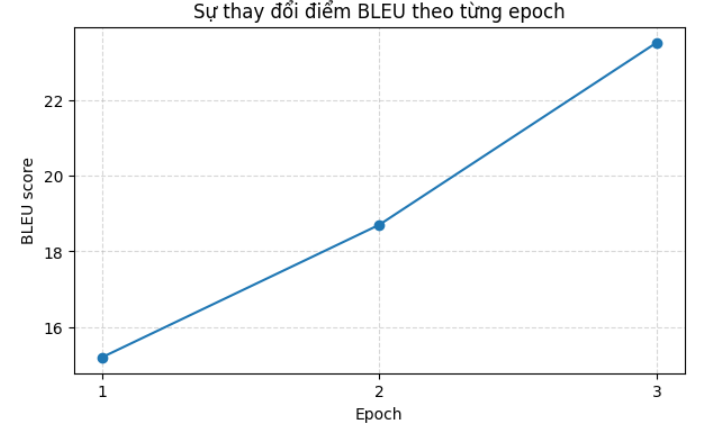
\includegraphics[width=0.78\textwidth]{figures/Anh/BLEU.png}
\caption{Sự thay đổi BLEU của mô-đun dịch Việt -- Lào theo từng epoch}
\label{fig:translation-bleu-epochs}
\end{figure}

\subsubsection{Nhận xét dựa trên trạng thái repository hiện tại}

Tại thời điểm viết báo cáo, snapshot mã nguồn hiện có:
\begin{itemize}
    \item bộ dữ liệu train/validation/test đã chia sẵn;
    \item adapter LoRA đã huấn luyện;
    \item script suy luận cho từng câu đầu vào.
    \item tài liệu \texttt{vilo.pdf} ghi nhận Train loss = 4,67, Validation loss = 1,06 và BLEU = 23,57.
\end{itemize}

Kết quả BLEU = 23,57 cho thấy mô hình đã học được khả năng dịch tương đối cho cặp Việt -- Lào, đặc biệt trong bối cảnh dữ liệu song ngữ ít tài nguyên hơn các cặp ngôn ngữ phổ biến. Tuy nhiên, mức BLEU này chưa phải chất lượng cao tuyệt đối; khi triển khai thực tế vẫn cần đánh giá thêm bằng ví dụ định tính và kiểm tra lỗi trên các câu dài, tên riêng, số và câu khẩu ngữ.

Trong workspace hiện tại chưa thấy số liệu chrF và TER tương ứng với cùng lần đánh giá. Vì vậy, cách trình bày trung thực nhất trong báo cáo là:
\begin{itemize}
    \item mô tả rõ mô hình đang dùng là \texttt{NLLB-200 Distilled 600M + LoRA};
    \item công bố các số liệu có nguồn trong \texttt{vilo.pdf}: Train loss, Validation loss và BLEU;
    \item giữ chrF và TER ở mức giao thức đề xuất, chưa công bố số nếu chưa tái lập được phép đo;
    \item tránh bịa thêm số liệu không có khả năng truy vết trong workspace.
\end{itemize}

Điểm này không phải là thiếu sót về học thuật, miễn là báo cáo ghi rõ trạng thái hiện tại và
không trình bày các con số không có khả năng truy vết.

\subsubsection{Đánh giá định tính nên nhấn mạnh điều gì}

Ngay cả khi đã có BLEU, chrF và TER, phần dịch Việt -- Lào vẫn cần thêm một bảng ví
dụ để người đọc thấy những kiểu lỗi quan trọng. Các nhóm ví dụ ưu tiên gồm:
\begin{itemize}
    \item câu nhu cầu cơ bản ngắn, ví dụ \textit{Tôi muốn uống nước};
    \item câu có tên riêng như bệnh viện, địa danh, tên người;
    \item câu dài hơn có mệnh đề phụ, ví dụ câu mô tả tình trạng sức khỏe hoặc yêu cầu trợ
    giúp;
    \item câu chứa số, thời gian hoặc thực thể viết hoa.
\end{itemize}

Quan sát nhanh trên dữ liệu song ngữ hiện có cho thấy các điểm rủi ro lớn nhất của mô-đun
dịch là:
\begin{itemize}
    \item tên riêng và từ phiên âm dễ bị sai hình thức;
    \item câu dài dễ lặp lại hoặc diễn đạt rườm rà;
    \item dữ liệu huấn luyện nhiều miền có thể làm mô hình không đồng đều chất lượng giữa
    các kiểu câu.
\end{itemize}

\subsubsection{Ý nghĩa của đánh giá đối với toàn hệ thống}

Mô-đun dịch là tầng cuối cùng trước khi thông tin đến tay người dùng đích. Vì vậy, nếu
mô-đun này dịch sai nghĩa, toàn bộ giá trị của pipeline trước đó có thể bị giảm mạnh. Đó là
lý do phần đánh giá dịch Việt - Lào cần được xem như một bước kiểm chứng độc lập và
đồng thời là một bước kiểm chứng cho chất lượng của cả hệ thống end-to-end.


\subsection{Đánh giá tích hợp toàn hệ thống}

Ngoài việc đánh giá độc lập từng mô hình, đề tài cần đánh giá pipeline tổng thể để phản ánh đúng giá trị ứng dụng thực tế. Đánh giá end-to-end không chỉ quan tâm từng nhãn ký hiệu có đúng hay không, mà còn xem câu tiếng Việt và câu tiếng Lào cuối cùng có truyền đạt đúng ý định ban đầu của người dùng hay không.

\subsubsection{Nội dung nên đánh giá}
\begin{itemize}
    \item Độ đúng của đầu ra cuối cùng từ video đến câu tiếng Việt và tiếng Lào.
    \item Tốc độ phản hồi của toàn pipeline.
    \item Tính ổn định của hệ thống khi chạy webcam liên tục.
    \item Ảnh hưởng của lỗi mô-đun trước lên mô-đun sau.
\end{itemize}

\begin{table}[H]
\centering
\caption{Đánh giá định tính pipeline end-to-end}
\label{tab:end-to-end-qualitative}
\begin{tabularx}{\textwidth}{|X|p{3.4cm}|X|}
\hline
\textbf{Kịch bản thử nghiệm} & \textbf{Kết quả} & \textbf{Nhận xét} \\
\hline
Người dùng ký hiệu câu ngắn, gồm 1--2 token & Khả thi trong demo & Khi token nhận diện đúng và có rule/fallback phù hợp, hệ thống sinh được câu tiếng Việt rõ nghĩa và có thể chuyển sang tầng dịch. \\
\hline
Người dùng ký hiệu nhiều token liên tiếp & Cần thao tác xác nhận & Chất lượng phụ thuộc mạnh vào việc chọn đúng token vào buffer; sai một token có thể làm câu tiếng Việt lệch nghĩa. \\
\hline
Điều kiện ánh sáng yếu hoặc tay ra khỏi khung hình & Không ổn định & Tầng nhận diện là điểm nghẽn chính; khi landmarks mất ổn định, toàn bộ pipeline phía sau bị ảnh hưởng. \\
\hline
Chạy không tải mô hình dịch & Ổn định hơn & Tùy chọn \texttt{--no-translation} phù hợp để kiểm thử nhanh hai tầng đầu hoặc chạy trên máy hạn chế tài nguyên. \\
\hline
Chạy đầy đủ có dịch Việt -- Lào & Phụ thuộc tài nguyên máy & Lần chạy đầu có thể cần tải mô hình nền NLLB; độ trễ cao hơn so với chỉ sinh câu tiếng Việt. \\
\hline
\end{tabularx}
\end{table}

Kết quả tích hợp cho thấy điểm quan trọng nhất của hệ thống là khả năng nối được ba mô-đun vốn có bản chất khác nhau: thị giác, sinh câu tiếng Việt và dịch máy. Tuy nhiên, đây vẫn là nguyên mẫu có người vận hành hỗ trợ xác nhận token. Để đạt mức sản phẩm hoàn chỉnh, hệ thống cần thêm cơ chế tự động tách câu, lọc dự đoán nhiễu, đánh giá ngưỡng tin cậy và kiểm thử trên nhiều người dùng thật.


\subsection{Kết luận đề tài}

Đề tài đã hiện thực hóa được một pipeline đa mô-đun cho bài toán hỗ trợ giao tiếp bằng ngôn ngữ ký hiệu, gồm ba tầng chính: nhận diện ký hiệu từ webcam, khôi phục câu tiếng Việt từ chuỗi gloss/token và dịch câu tiếng Việt sang tiếng Lào. Cách tiếp cận này chứng minh tính khả thi của việc kết hợp thị giác máy tính, xử lý ngôn ngữ tự nhiên và dịch máy trong cùng một hệ thống ứng dụng.

Ở tầng nhận diện, hệ thống tích hợp thành công mô hình TFLite pre-trained từ Kaggle ASL Signs với MediaPipe Holistic, sử dụng toàn bộ 543 landmarks và cơ chế cửa sổ trượt 16--60 frame. Nhóm đã bổ sung công cụ đánh giá để tính Top-k Accuracy, Precision, Recall, F1 và confusion matrix khi có tập kiểm thử gán nhãn; trong snapshot hiện tại chỉ công bố latency TFLite vì chưa có test manifest nhận diện riêng. Ở tầng tiếng Việt, hệ thống sử dụng kiến trúc lai gồm rule, BARTpho và fallback để chuyển chuỗi token thành câu tiếng Việt hoàn chỉnh. Kết quả đánh giá trên tập test của mô-đun tiếng Việt cho thấy các metric đạt mức rất cao trong miền dữ liệu được thiết kế. Ở tầng dịch, hệ thống tích hợp NLLB-200 Distilled 600M với adapter LoRA cho cặp Việt -- Lào; tài liệu \texttt{vilo.pdf} ghi nhận Train loss = 4,67, Validation loss = 1,06 và BLEU = 23,57.

Về mặt học thuật, đề tài giúp hệ thống hóa quy trình xây dựng một ứng dụng AI nhiều tầng, trong đó mỗi mô hình có vai trò, dữ liệu và metric đánh giá riêng. Về mặt ứng dụng, project tạo được nguyên mẫu có thể chạy demo từ webcam, có cơ chế buffer token và có khả năng bật/tắt tầng dịch tùy theo tài nguyên máy. Những kết quả này đáp ứng mục tiêu ban đầu của đề tài ở mức nguyên mẫu nghiên cứu và là nền tảng để mở rộng thành hệ thống thực tế hơn trong tương lai.


\subsection{Hạn chế hiện tại}

Mặc dù hệ thống đã nối được ba mô-đun chính, phiên bản hiện tại vẫn còn một số hạn chế cần được nhìn nhận thẳng thắn.

\begin{itemize}
    \item Mô hình nhận diện đang dùng bộ ASL-250 pre-trained, chưa phải mô hình VSL thuần được huấn luyện trên dữ liệu người dùng Việt Nam.
    \item Chất lượng nhận diện còn nhạy với ánh sáng, góc quay, khoảng cách tới camera, che khuất tay và tốc độ ký hiệu.
    \item Pipeline hiện nhận diện theo token/gloss có thao tác xác nhận, chưa xử lý hoàn toàn tự động câu ký hiệu liên tục dài.
    \item Sai số ở tầng nhận diện có thể lan sang tầng khôi phục câu và tầng dịch, đặc biệt khi một token quan trọng bị nhận sai.
    \item Metric của mô-đun tiếng Việt rất cao trên bộ dữ liệu có cấu trúc/template, nhưng chưa đủ để khẳng định chất lượng tương đương trên dữ liệu giao tiếp tự do.
    \item Mô-đun dịch Việt -- Lào đã có Train loss, Validation loss và BLEU trong \texttt{vilo.pdf}, nhưng chưa có chrF và TER truy vết trong workspace nên cần tái lập thêm nếu muốn đánh giá đầy đủ hơn.
    \item Hệ thống hiện mới dừng ở mức nguyên mẫu demo, chưa được đóng gói thành ứng dụng desktop/web/mobile hoàn chỉnh.
\end{itemize}


\subsection{Hướng phát triển}

Trên cơ sở các hạn chế hiện tại, đề tài có thể được phát triển theo nhiều hướng nhằm nâng cao cả độ chính xác lẫn khả năng ứng dụng thực tế.

\begin{itemize}
    \item Thu thập hoặc xây dựng bộ dữ liệu VSL thật với nhiều người ký hiệu, nhiều góc quay và nhiều điều kiện ánh sáng để huấn luyện/fine-tune mô hình nhận diện phù hợp hơn với tiếng Việt.
    \item Xây dựng tập kiểm thử nhận diện có nhãn thật và file manifest \texttt{path,label} để công bố đầy đủ Top-1, Top-3, Top-5 Accuracy, Macro F1 và confusion matrix cho tầng thị giác.
    \item Mở rộng số lớp ký hiệu và bổ sung cơ chế nhận diện câu ký hiệu liên tục, bao gồm tách đoạn động tác, lọc nhiễu và gom token tự động.
    \item Thử nghiệm các mô hình chuỗi hoặc video mạnh hơn như Transformer-based video models, Temporal Convolution hoặc Graph Neural Network trên landmarks.
    \item Cải thiện mô-đun khôi phục câu bằng dữ liệu gloss -- câu phong phú hơn, đặc biệt là dữ liệu sinh từ lỗi thật của tầng nhận diện.
    \item Tái lập đánh giá đầy đủ cho mô-đun dịch Việt -- Lào trên validation/test set, lưu log metric và bổ sung đánh giá thủ công bởi người biết tiếng Lào.
    \item Bổ sung text-to-speech cho tiếng Việt hoặc tiếng Lào để hệ thống hỗ trợ giao tiếp bằng giọng nói.
    \item Đóng gói thành ứng dụng desktop, web hoặc mobile, kèm giao diện thân thiện hơn và cơ chế cấu hình camera/mô hình.
\end{itemize}



\clearpage


\section*{TÀI LIỆU THAM KHẢO}
\addcontentsline{toc}{section}{TÀI LIỆU THAM KHẢO}

\begingroup
\sloppy
\begin{enumerate}
    \item TS. Lê Quốc Uy, \textit{Slide bài giảng học phần Học Sâu}, Khoa Kỹ Thuật Điện Tử 1, Học viện Công nghệ Bưu chính Viễn thông.

    \item Camillo Lugaresi, Jiuqiang Tang, Hadon Nash, Chris McClanahan, Esha Uboweja, Michael Hays và cộng sự, \textit{MediaPipe: A Framework for Building Perception Pipelines}, arXiv 2019. URL:
    \url{https://arxiv.org/abs/1906.08172}.

    \item Google, \textit{MediaPipe Holistic Documentation}. Truy cập tại:
    \url{https://ai.google.dev/edge/mediapipe/solutions/vision/holistic_landmarker}.

    \item Dongxu Li, Cristian Rodriguez Opazo, Xin Yu và Hongdong Li, \textit{Word-level Deep Sign Language Recognition from Video: A New Large-scale Dataset and Methods Comparison}, WACV 2020. URL:
    \url{https://openaccess.thecvf.com/content_WACV_2020/papers/Li_Word-level_Deep_Sign_Language_Recognition_from_Video_A_New_Large-scale_WACV_2020_paper.pdf}.

    \item Sepp Hochreiter và Jürgen Schmidhuber, \textit{Long Short-Term Memory}, Neural Computation, 1997. URL:
    \url{https://direct.mit.edu/neco/article/9/8/1735/6109/Long-Short-Term-Memory}.

    \item Mike Schuster và Kuldip K. Paliwal, \textit{Bidirectional Recurrent Neural Networks}, IEEE Transactions on Signal Processing, 1997. URL:
    \url{https://deeplearning.cs.cmu.edu/S22/document/readings/Bidirectional%20Recurrent%20Neural%20Networks.pdf}.

    \item Mike Lewis, Yinhan Liu, Naman Goyal, Marjan Ghazvininejad, Abdelrahman Mohamed, Omer Levy, Ves Stoyanov và Luke Zettlemoyer, \textit{BART: Denoising Sequence-to-Sequence Pre-training for Natural Language Generation, Translation, and Comprehension}, ACL 2020. URL:
    \url{https://arxiv.org/abs/1910.13461}.

    \item Nguyen Luong Tran, Duong Minh Le và Dat Quoc Nguyen, \textit{BARTpho: Pre-trained Sequence-to-Sequence Models for Vietnamese}, INTERSPEECH 2022. URL:
    \url{https://arxiv.org/abs/2109.09701}.

    \item NLLB Team, Marta R. Costa-juss\`{a}, James Cross, Onur \c{C}elebi và cộng sự, \textit{No Language Left Behind: Scaling Human-Centered Machine Translation}, 2022. URL:
    \url{https://arxiv.org/abs/2207.04672}.

    \item Edward J. Hu, Yelong Shen, Phillip Wallis, Zeyuan Allen-Zhu, Yuanzhi Li, Shean Wang, Lu Wang và Weizhu Chen, \textit{LoRA: Low-Rank Adaptation of Large Language Models}, 2021. URL:
    \url{https://arxiv.org/abs/2106.09685}.

    \item Hugging Face, \textit{NLLB Model Documentation}. Truy cập tại:
    \url{https://huggingface.co/docs/transformers/model_doc/nllb}.

    \item Kishore Papineni, Salim Roukos, Todd Ward và Wei-Jing Zhu, \textit{BLEU: a Method for Automatic Evaluation of Machine Translation}, ACL 2002. URL:
    \url{https://aclanthology.org/www.mt-archive.info/ACL-2002-Papineni.pdf}.

    \item Chin-Yew Lin, \textit{ROUGE: A Package for Automatic Evaluation of Summaries}, Workshop on Text Summarization Branches Out, 2004. URL:
    \url{https://aclanthology.org/W04-1013/}.

    \item Maja Popovi\'{c}, \textit{chrF: character n-gram F-score for automatic MT evaluation}, WMT 2015. URL:
    \url{https://aclanthology.org/W15-3049/}.

    \item Matthew Snover, Bonnie Dorr, Rich Schwartz, Linnea Micciulla và John Makhoul, \textit{A Study of Translation Edit Rate with Targeted Human Annotation}, AMTA 2006. URL:
    \url{https://aclanthology.org/2006.amta-papers.25/}.

    \item Mahya Fayyazsanavi, Ruwanthi Attanayake và Richard Bowden, \textit{Gloss2Text: Sign Language Gloss Translation using LLMs and Semantically Aware Label Smoothing}, Findings of EMNLP 2024. URL:
    \url{https://aclanthology.org/2024.findings-emnlp.947/}.

    \item Kaggle, \textit{Google -- Isolated Sign Language Recognition Competition}. Truy cập tại:
    \url{https://www.kaggle.com/competitions/asl-signs}.

    \item hoyso48, \textit{1st Place Solution -- Inference}, Kaggle ASL Signs Competition. Truy cập tại:
    \url{https://www.kaggle.com/code/hoyso48/1st-place-solution-inference}.

    \item Google, \textit{TensorFlow Lite Documentation}. Truy cập tại:
    \url{https://www.tensorflow.org/lite}.
\end{enumerate}
\endgroup



\end{document}

